\part{\FPTIME{}}

\chapter{A Generalised Framework}

\begin{quotation}

\footnotesize\sffamily\itshape

\begin{flushright}

{\upshape PETER HILTON} \\
Christ!! What happens now?!\\
{\upshape ALAN TURING} \\
It should tell use the day's Enigma settings!\\
{\upshape HUGH ALEXANDER} \\
How long!?!

\smallbreak

\upshape

--- Graham More, The Imitaiton Game (2014)

\end{flushright}

\end{quotation}

\todo{Stop reading here and go to \refSec{generalised-projection}.}

The fundamental insight highlighted by the above quotation underpins much work
done in \cite{jones-1999, jones-2001, kristiansen-voda-2005, hofmann-2003,
kristiansen-2008}, and of course, \cite{jones-kristiansen-2009}, among others.
We draw on this insight in a fundamental and perhaps extreme way, by taking the
notion of ``successor-like function'' to roughly mean ``enumerator'', and
consider the presence and absence of both particular successor-like \emph{and}
predecessor-like functions.

Implicit characterizations of complexity classes, e.g. PTIME, often start out
by considering first-order programs on natural numbers. That is, the
computation of (mathematical) functions of type $\mathbb{N} \rightarrow
\mathbb{N}$. (For a counterexample, see \cite{hofmann-2003}.) 

In lieu of \refThm{tm-total}, such results apply even if we replace
$\mathbb{N}$ (on either side) by any countable or countably infinite set. That
is, the results still hold even if we turn to the computation of (mathematical)
functions of type $A \rightarrow B$ for some countable or countably infinite
sets $A$ and $B$.

Crucially, \refThm{tm-total} relies on \emph{mathematical} functions, not
real-world transformations. Realistically, all we get is this: assuming that we
have a representation of a value of type $A$ as a natural number, we can
compute a natural number representation of the corresponding value of type $B$,
within the characterised bounds.

This outset of ``first-order programs on natural numbers'' ignores the
real-life hurdle of dealing with \emph{data structures} rather than natural
numbers. So such an exposition is arguably impractical, or more dramatically,
ignores certain \emph{complexities} involved in dealing with data.

Instead, we formalise a notion of ``successor'' and ``predecessor'', and
present seminal results in the characterisation of PTIME in terms of this
general framework. Informally, a successor or predecessor is any operation that
may change the size of any value in the program (including time?). In practice,
essentially any conceivable operation, except perhaps stalling.

\section{Programs}

% Many high-level programming languages have data types, and these data types
% cannot be coerced.

In the interest of capturing a wide range of programming paradigms in one
discussion, we give only a general specification of what we deem a program to
be. This specification will later be specialized for more concrete purposes. We
make no claim however, that in so doing, we capture all conceivable programming
paradigms.

\begin{specification}

A \textbf{program} $P = \p{P_\mathbf{D}, P_\mathbf{F}}$ is a finite set of
\textbf{data types} $P_\mathbf{D}$, and a finite set of \textbf{functions}
$P_\mathbf{F}$, subject to the following laws:

\begin{enumerate}

\item [P-1] Every data type $A \in P_\mathbf{D}$ forms a set.

\item [P-2] Every function $f \in P_\mathbf{F}$ computes a partial function $f
: A \rightharpoonup B$, for some $A, B\in P_\mathbf{D}$. We write $f : A
\rightharpoonup B \in P_\mathbf{F}$.

\item [P-3] For every data type $A \in P_\mathbf{D}$ there is a \textbf{size
function} $\card{\cdot} : A \rightarrow \mathbb{N}$, so for every $a \in A$ we
have $\card{a} \in \mathbb{N}$.

\end{enumerate}

\end{specification}

\begin{remark} We do not require that a function $f \in P_\mathbf{F}$ can
compute a partial function $f : A \rightharpoonup B$ between \emph{any} given
data types $A, B \in P_\mathbf{D}$, merely that it is a partial function
between \emph{some} given data types $A, B \in P_\mathbf{D}$.  \end{remark}

\begin{remark} The purpose of the size function is primarily semantic, and so
it need not be in $P_\mathbf{F}$, but of course, it could be. \end{remark}

\subsection{Successors and Predecessors}

\begin{definition} A partial function $s : X \rightharpoonup Y \in
P_\mathbf{F}$ is a \textbf{successor function} for some $x \in X$ iff $s\p{x}$
is defined and $\card{x} < \card{s\p{x}}$. \end{definition}

\begin{definition} A partial function $p : X \rightharpoonup Y \in
P_\mathbf{F}$ is a \textbf{predecesor function} for some $x \in X$ iff $p\p{x}$
is defined and $\card{p\p{x}} < \card{x}$. \end{definition}

That is, a successor function produces an output \emph{strictly greater} in
size than its input, and a predecessor function produces an output
\emph{strictly lesser} in size than its input.

Note in particular, that whether a given partial function $f : X
\rightharpoonup Y \in P_\mathbf{F}$ is a successor or predecessor function, if
either, \emph{depends} on the value $x \in X$ which $f$ is applied to. If $X$
is a countably infinite data type, there may exist functions which are
successor functions, \emph{independent} of the value that they are applied to.

\begin{definition} A partial function $c : X \rightharpoonup Y \in
P_\mathbf{F}$, is a \textbf{constructor} iff $X$ is the domain of definition of
$c$, so $c : X \rightarrow Y \in P_\mathbf{F}$, and $c$ is a successor function
\emph{for all} $x \in X$. \end{definition}

On the other hand, for any data type $X$, there must exist some value $x \in
X$, for which any given function is \emph{not} a predecessor function, as
otherwise there would be a natural number less than $0$.

\subsection{Defining Functions}

For the purposes of a further discussion about programming, we adopt an
equational programming style, in line with classical recursion theory and
functional programming.

\begin{definition} For any program $P = \p{P_\mathbf{D}, P_\mathbf{F}}$, let
$P_\mathbf{F}$ form the \textbf{signature} of $P$, that is, for every $f : X
\rightharpoonup Y \in P_\mathbf{F}$, we say that $f$ is a \textbf{symbol}, and
$X \rightharpoonup Y$ is the \textbf{arity} of symbol $f$. \end{definition}

\begin{definition} A \textbf{variable} $v$ of type $Y \in P_\mathbf{D}$, is a
symbol $v$, which does not occur in $P_\mathbf{F}$. \end{definition}

\begin{definition} A \textbf{term} $t$ of type $Y$, written $t : Y$, is either
a variable $t \equiv v$, or a \textbf{compound term} $t \equiv f\p{x}$, where
$f : X \rightharpoonup Y$ and $x \in X$. \end{definition} 

\begin{definition} A \textbf{ground term} $t : Y$, is a either a variable $t
\equiv v$, or a compound term $t \equiv f\p{x}$, where $f : X \rightharpoonup
Y$ is a \emph{constructor} and $x : X$ is also a \emph{ground term}.
\end{definition}

\begin{definition} If $x$ is a ground term and $y$ is a term, then $x \leadsto
y$ is a \textbf{clause}.  \end{definition}

\begin{remark} We deviate from the classical use of the symbol $=$ (equals),
frequent in recursion theory and functional programming. We are not concerned
with any notion of ``equality'' between the left- and right-hand side of a
clause. Instead, a clause should state how the left-hand side \emph{leads to}
the right hand side. That is, we have chosen which way evaluation flows. To the
acute reader this sounds an awful lot like term-rewriting, and though it is, we
see no need to dive further into term-rewriting terminology. \end{remark}

\begin{definition} A function is given by a finite set of clauses, where no
pair of left-hand sides unify using the conventional algorithm.
\end{definition}

\subsection{Examples}

\begin{example} Peano numbers in one programming language or another. Model
theory? \end{example}

\subsection{Programming with algebraic data types}

To this end we adopt the notation of \cite{marion-2003}.

\begin{definition} A \textbf{sort} $\mathcal{S}$ is a set. \end{definition}

\begin{specification} The set of \textbf{types} $\mathcal{T}$ over a sort
$\mathcal{S}$ is  built from either the elements of $\mathcal{S}$ or
\textbf{type constructors}. \end{specification}

\begin{definition} A \textbf{vocabulary} is a set of symbols \end{definition} 

We follow the approach and notation of \cite{clote-1999}, where many of the
below results are presented using a single-sorted word algebra. We consider
generalizing the presentation to many-sorted algebras where this has already
been done by others, and otherwise.

A recursion scheme will be given over a particular algebra, where an algebra is
given over a signature.

\begin{definition} A \textbf{signature} is a triple $\Sigma = \p{\mathbf{B},
\mathbf{T}, \mathbf{C}}$, where

\begin{enumerate}

\item [$\mathbf{B}$] is a set of \textbf{base types},

\item [$\mathbf{T}$] is a set of \textbf{type constructors}, and

\item [$\mathbf{V}$] is a set of \textbf{value constructors}.

\end{enumerate}

\end{definition}

The set of base types and type constructors can be deduced from the set of
value constructors in a signature. We choose to mark these elements in a
distinct manner to make the following notions straight forward to discuss.

\begin{definition} A signature is \textbf{single-sorted} if it has exactly one
base type $B$, written $\Sigma = \p{\set{B}, -, -}$. A signature that is not
single-sorted is \textbf{many-sorted}.  \end{definition}

\begin{definition} For a set of base types $\mathbf{B}$, let $*$ denote any
base type in $\mathbf{B}$. \end{definition}

\begin{definition} A \textbf{word} signature is a signature having just the
type constructors $*$ and $* \rightarrow *$, written $\p{\mathbf{B}, \set{*, *
\rightarrow *}, \mathbf{V}}$.  \end{definition}

% \begin{example} A single-sorted word signature is a signature $\p{\set{B},
% \set{*, * \rightarrow *}, \mathbf{V}}$. That is, for each $v \in \mathbf{V}$
% we either have $v : B$ or $v : B\rightarrow B$. \end{example}

As an example, we now turn to the Peano numbers:

\begin{definition} The \textbf{Peano numbers} is the single-sorted word
signature

$$\Pi \triangleq \p{\set{N}, \set{*, * \rightarrow *}, \set{\mathtt{z} : N,
\mathtt{s} : N \rightarrow N}}.$$

\end{definition}

% \begin{definition} A \textbf{tree} algebra is an algebra having the type
% constructors $\mathbf{T} = \set{*, \mathbf{T} \rightarrow \mathbf{T}}$,
% written $\p{\mathbf{B}, \mathbf{T} = \set{*, \mathbf{T} \rightarrow
% \mathbf{T}}, \mathbf{V}}$. \end{definition}

% \begin{example} A single-sorted binary tree algebra is an algebra over the
% signature $\p{\set{B}, \set{*, * \rightarrow * \rightarrow *}, \mathbf{V}}$,
% where for each $v \in \mathbf{V}$ we either have $v : B$ or $v : B\rightarrow
% B \rightarrow B$. \end{example}

\begin{definition} The set of \textbf{$n$-ary} value constructors over $\Sigma
= \p{-, -, \mathbf{V}}$ is

$$\mathbf{V}_n \triangleq \set{v \in \mathbf{V} \st{v : *_0 \rightarrow *_1
\rightarrow \cdots \rightarrow *_n}}$$

\end{definition}

\begin{definition} The set of \textbf{constructor terms} over
$\Sigma=\p{-, -, \mathbf{V}}$ is

$$\mathcal{C}_\Sigma \triangleq \set{v\p{t_1,t_2,\ldots,t_n} \st{n \in
\mathbb{N} \wedge v \in \mathbf{V}_n \wedge t_1,t_2,\ldots,t_n \in
\mathcal{C}_\Sigma}}$$

\end{definition}

\begin{example} The set of constructor terms over the Peano numbers is

$$\mathcal{C}_\Pi = \set{\mathtt{z}, \mathtt{s}\p{\mathtt{z}},
\mathtt{s}\p{\mathtt{s}\p{\mathtt{z}}},
\mathtt{s}\p{\mathtt{s}\p{\mathtt{s}\p{\mathtt{z}}}}, \ldots}$$

\end{example}

% recursive call stack

% purely functional programs? no data other than what you put in.

% Perhaps a neat way of categorise the wealth of data structures 

% We take a programming languages approach, and in the process relax a couple
% terms from modern programming nomenclature.

% \begin{definition} A \textbf{program} is a countable set of functions.
% \end{definition}

% \begin{definition} For a given program, let the \textbf{$A$-valued functions}
% be all the functions in $P$ with codomain $A$. \end{definition}

% \begin{definition} A \textbf{data type} $A$ is given by a subset $S$ of the
% $A$-valued functions $T$, such that all functions in $T \setminus S$ return
% values constructed using functions in $S$. The functions in $S$ are called
% \textbf{value constructors}. \end{definition}

% \begin{remark} Typically, the value constructors are defined in a language
% using designated syntax. \end{remark}

% \begin{remark} For the functional programmer this is a degeneration of the
% common term ``value constructor''. For her, a data type is defined by a
% finite set of well-placed value constructors, and can only be constructed
% using these value constructors. Value constructors are $O(1)$-time and
% $O(1)$-space operations, each having an inverse ``value deconstructor'' for
% use in e.g.  pattern matching. For the imperative programmer, this is a
% degeneration of the common term ``constructor''. Here we lend the term from
% C++, where a type can have multiple constructors taking an arbitrarily long
% time and space, and having at least one common (but perhaps multiple)
% inverses. \end{remark}

% Typically a value constructor has an inverse: a value deconstructor.

% In the presence of successors without pairing predecessors, we must do away
% with such notions.

% \begin{notation} Let $P_\mathbf{D}$ denote the data types induced by the
% functions of program $P$, that is, the set of all codomains in $P$.
% \end{notation}

% \begin{definition} A value constructor is a \textbf{successor} \end{definition} 

% Cobham: Let a function $f$ be defined by a range of base case clauses, and a
% range of deconstructor clauses. The recursive clauses may use various
% predecessor operations.

% Size is always given relative to a particular predecessor operation.

% Consider the predecessor (among those used in the function) that decreases
% the value by the least amount. Assume that the predecessors are always
% applicable to a given value, and that by iterated use of the predecessor, we
% reach a base case. A function is defined by bounded primitive recursion, if
% the number of applications of this most-basic predecessor is no more than as
% given by the given bound.

% Also, better suited as an introduction as it doesn't really say anything
% about the choice of polynomial time from the get go. That's more a
% coincidence, the following definitions will hold regardless. Perhaps it is
% worth it calling this a Part I: Introduction and Background

% Fragment of a logic means that we are restricted to a subset of the syntax,
% but retain the same semantics. If we choose the combination of words -
% subsystem of system, we are perhaps a little more free, but in either case,
% we probably have to further specify what we keep and what we take out.

% for the purposes of this thesis, we may regard logical systems equivalent to
% programming languages - draw inspiration from Types of Crash Prevention - it
% has a nice, human readable introduction to the whole thing.

% The correspondence between an ICC system and a complexity class is
% extensional, i.e. the class of function (or problems) representable in the
% system equals the complexity class.

% by this point we should have more precisely defined the notions of function
% and problem.

% The systems that we will consider here will be subsystems of a larger base
% system, in which other functions, besides those in the complexity class of
% the system can be represented.

% \begin{definition} \textit{Intensional soundness}

% Any program representable in the ICC system, is within the given complexity
% class. Proven by showing equivalence of the class of problems to a complexity
% class.

% \end{definition}

% \begin{definition} \textit{Intensional completeness}

% All functions in the complexity class are representable in the ICC system.

% \end{definition}

% \begin{definition} \textit{Extensional soundness}

% All functions in the complexity class are representable in the base system.

% \end{definition}




% we want natural numbers, but we don't want the successor and predecessor
% operations to always be blindly permitted.

% primitive recursion is really defined in terms of a predecessor operation, at
% least if we assume the successor operation to merely be something that can
% construct a "bigger" value. otherwise, it is undefined how in primitive
% recursion we first compute the lower-order value.

% we run into the same problem with s_1 and s_0! Does it at all make sense to
% define a successor without a predecessor? At least not if we want to be able
% to define functions recursively! Any time we define a function computing a
% bigger value having a lower value, we need to specify it in terms of
% predecessors!

% decrement on binary notation is a polynomial-time operation if we only assume
% s_0 and s_1 (or rather, their predecessors). We can assume dec to be a
% unit-cost operation, and that is where the problems of primitive recursion
% creep up.

% although we can always convert a unique string to a unique natural number, it
% may take a long time to do so. Furthermore, the successor operation is a
% polynomial time oper

% Any more definite attempt at a definition of the natural numbers seems to
% arrive at a philosophical impasse.

% The natural numbers have never-the-less shown to be of prime importance due to
% the concept of recursive enumerability.

% Use sets rather than ``language'' to avoid mixing up inputs/outputs of
% machines and the programming languages that we design. Languages refer
% specifically to sets of strings.

% \begin{definition}

% Define enumerator.

% \end{definition}

% \begin{definition}

% Define recursively enumerable sets.

% \end{definition}

% Dealing with natural numbers is bad as we would quickly regard the successor
% (and predecessor) operations to be paired and unit-cost operations.

% You cannot take the successor operation to be a unit-cost operation, nor can
% you assume that it is paired with a predecessor.

% we are dealing with words? basic data elements on any machine model?

% an element of state in a machine model. it has an initial state, and some
% succeeding states - preceding states don't really make sense.

% a successor does not lead you to another state

% at least size is not defined in terms of the number states that you've passed.

% for all classical machine models, the class of polynomial-time computable
% functions is equivalent.

% the values of any practical data structure can be recursively enumerated; so
% although the fact that a set is recursively enumerable opens a pandoras box,
% only a practical subset of it will be used in practice.

% this is an explanation of godel encoding.

% strings or states of a data structure?

% due to godel encoding, it is okay to deal in natural numbers, provided that
% we do not (necessarily) permit a unit-cost unique successor operation.

% so we're actually redefining natural numbers again? - yes.

% the natural numbers that you do have in any programming language, depend on
% the constructs available in your language. indeed, due to godel encoding, any
% practical programming languages comes with manifolds of ways of defining
% natural numbers.

% is all this because we want to deal in the natural numbers?

% In practice, we often deal with recursive sets, as by the Church-Turing thesis,
% these are  the computable functions. This makes it attractive to deal merely in
% the natural numbers as introduced above. Although this is perhaps a useful
% definition of natural numbers, the pairing of a recursively enumerable set with
% the natural numbers can be a rather complex procedure.

% We intend to model this complexity by permitting a more elaborate definition of
% natural numbers:

% \begin{notion}

% A \textbf{value} is either $0$, a successor, or a predecessor of a value. A
% successor and predecessor need not take $O(1)$ to compute.

% \end{notion}

% The notions of successor and predecessor are defined below.

% It is intentional that we do not denote the syntax of $x$.

% what is a data type?

% \begin{definition}

% The \textbf{notation} of a particular data type is a specification of how
% values of that data type may be constructed and deconstructed.

% \end{definition}

% \section{Successors}

% multiple possible successor and predecessor functions.

% TODO: define <, =, \vdash

% to define <, we need to define size; so < is defined for some measure of size.

% The rules with < occurring so early is not a problem as it is a statement
% that these rules must hold, either as part of the definition of a successor
% s, or as an admissible rule.

% \begin{definition}

% A function $s$ is a \textbf{successor} function iff

% \begin{align}
% &\vdash 0 < s(x) \\
% x < y &\vdash s(x) < s(y)
% \end{align}

% \end{definition}

% Successor functions play a key role in the remainder of the thesis, as they
% form the basis of our measure of the size of a value.

% \begin{definition}

% The \textbf{size} of a value $x$, the minimum number of successor
% applications necessary to construct $x$.

% \end{definition}

% For instance, a language $\mathcal{B}$ that uses binary notation may have two
% successors, one that doubles the value, $s_0$, and another that doubles the
% value and adds a one, $s_1$. The value $5$ is then represented in
% $\mathcal{B}$ as $s_1\p{s_0\p{s_1\p{0}}}$, and so the size of the value $5$
% in $\mathcal{B}$ is $3$. Analytically, the size of a value $x$ in
% $\mathcal{B}$ is $\ceil{\log_2\p{x}}$.

% \section{Predecessors}

% \begin{definition}

% A function $p$ is a \textbf{predecessor} function iff

% no cycles?

% \begin{align}
% &\vdash p\p{0} = 0 \\
% &\vdash p\p{x} < x & x \neq 0 \\
% x < y &\vdash p\p{x} < p\p{y}
% \end{align}

% \end{definition}

For instance, the language $\mathcal{B}$ above, may have a predecessor function
$dec$ (read: decrement) defined as follows:

\begin{align}
dec'\p{x}=y, trim\p{y}=z &\vdash dec\p{x} = z \\
dec'\p{x} = y &\vdash dec'\p{s_1\p{x}} = s_1\p{y} \\
dec''\p{x} = y &\vdash dec'\p{s_1\p{x}} = s_0\p{y} \\
dec'\p{x} = y &\vdash dec'\p{s_0\p{x}} = s_0\p{y} \\
dec''\p{x} = y &\vdash dec''\p{s_0\p{x}} = s_1\p{y} \\
&\vdash dec''\p{s_0\p{0}} = s_1\p{0} \\
&\vdash dec'\p{s_1\p{0}} = s_0\p{0} \\
&\vdash dec'\p{0} = 0 \\
trim\p{y} = z &\vdash trim\p{s_0\p{y}} = z \\
&\vdash trim\p{s_1\p{y}} = s_1\p{y} \\
&\vdash trim\p{0} = 0
\end{align}

For instance, $s_1\p{s_0\p{s_1\p{0}}}$, i.e. 5, decremented, is
$s_1\p{s_0\p{s_0\p{0}}}$, i.e. 4:

$$
\judgement{
  \judgement{
    \judgement{
      \axiom{
        dec'\p{s_1\p{0}} = s_0\p{0}
      }
    }{
      dec'\p{s_0\p{s_1\p{0}}} = s_0\p{s_0\p{0}}
    }
  }{
    dec'\p{s_1\p{s_0\p{s_1\p{0}}}} = s_1\p{s_0\p{s_0\p{0}}}
  }
  \quad
  \axiom{
    trim\p{s_1\p{s_0\p{s_0\p{0}}}} = s_1\p{s_0\p{s_0\p{0}}}
  }
}{
  dec\p{s_1\p{s_0\p{s_1\p{0}}}} = s_1\p{s_0\p{s_0\p{0}}}
}
$$

and $s_1\p{s_0\p{s_0\p{0}}}$, i.e. 4, decremented, is $s_1\p{s_1\p{0}}$, i.e. $3$:

$$
\judgement{
  \judgement{
    \judgement{
      \axiom{
        dec''\p{s_0\p{0}} = s_1\p{0}
      }
    }{
      dec''\p{s_0\p{s_0\p{0}}} = s_1\p{s_1\p{0}}
    }
  }{
    dec'\p{s_1\p{s_0\p{s_0\p{0}}}} = s_0\p{s_1\p{s_1\p{0}}}
  }
  \quad
  \judgement{
    \axiom{
      trim\p{s_1\p{s_1\p{0}}} = s_1\p{s_1\p{0}}
    }
  }{
    trim\p{s_0\p{s_1\p{s_1\p{0}}}} = s_1\p{s_1\p{0}}
  }
}{
  dec\p{s_1\p{s_0\p{s_0\p{0}}}} = s_1\p{s_1\p{0}}
}
$$

\section{Successors and predecessors}

\begin{definition}

A predecessor function $p$ is \textbf{paired} with a successor function $s$ iff

\begin{align}
\vdash p\p{s\p{x}} &= x
\end{align}

\end{definition}

It is not a requirement for a predecessor to be paired with a successor. A
language may have predecessors more powerful than any of its successors.

\begin{remark}

A successor or predecessor function may or may not take $O(1)$ time. This
depends on the machine model.

\end{remark}

\section{Primitive recursion}

\begin{definition}

A function is defined by \textbf{primitive recursion} (PR), from PR functions
$g$ and $h$, and a PR predecessor function $p$, iff

\begin{align}
f\p{0,\vect{y}} &= g\p{\vect{y}} \\
f\p{x, \vect{y}} &= h\p{x, \vect{y}, f\p{p\p{x},\vect{y}}}
\end{align}

\end{definition}

The running time of a PR function $f$, depends on the running times of $g$,
$h$, and $p$, as well as how quickly $p$ decreases $x$ to $0$.

Mere primitive recursion is not confined to polytime computation.

\begin{theorem}
PR is not confined to polytime computation.
\end{theorem}

\begin{proof} Assume that $g$, $h$, and $p$ are all computed in $O(1)$ time.
Consider the language $\mathcal{B}$ above, having just the successors $s_0$ and
$s_1$. Let $p$ be the function $dec$ above.\end{proof}

The trouble is that $p$ does not decrease $x$ fast enough throughout the
recursion --- the number of times $p$ has to be applied to $x$ to reach $0$, is
superpolynomial in $x$.

One attempt to mitigate for this could be to have $p$ decrease the value
faster. For instance, sticking with the language $\mathcal{B}$ above, we could
let $p$ be a function that halves $x$. This would pair $p$ with $s_0$.

\begin{theorem}

Primitive recursion defined with a predecessor function which is paired with a
successor function is not confined to polytime computation.

\end{theorem}

\begin{proof} Let a predecessor function $p$ be paired with a successor
function $s$.

Consider a function $dbl$, which doubles its input:

\begin{align}
dbl\p{0} &= 0 \\
dbl\p{x} &= s\p{s\p{dbl\p{p\p{x}}}}
\end{align}

Consider furthermore a function $iterdbl$, which calls $dbl$ iteratively, the
same number of times as the length of its input:

\begin{align}
iterdbl\p{0} &= s\p{0} \\
iterdbl\p{x} &= dbl\p{iterdbl\p{p\p{x}}}
\end{align}

Calling $iterdbl$ with a string of length $n$, we obtain a string of length
$2^n$ due to iterated doubling of the input. It follows that $iterdbl$ does a
superpolynomial amount of work in the size of its input.\end{proof}

\begin{example}
We illustrate the above proof with an example:
\begin{align}
\underline{iterdbl\p{s\p{s\p{0}}}}
  &\leadsto dbl\p{iterdbl\p{\underline{p\p{s\p{s\p{0}}}}}} \\
  &\leadsto dbl\p{\underline{iterdbl\p{s\p{0}}}} \\
  &\leadsto dbl\p{dbl\p{iterdbl\p{\underline{p\p{s\p{0}}}}}} \\
  &\leadsto dbl\p{dbl\p{\underline{iterdbl\p{0}}}} \\
  &\leadsto dbl\p{\underline{dbl\p{s\p{0}}}} \\
  &\leadsto dbl\p{s\p{s\p{dbl\p{\underline{p\p{s\p{0}}}}}}} \\
  &\leadsto dbl\p{s\p{s\p{\underline{dbl\p{0}}}}} \\
  &\leadsto \underline{dbl\p{s\p{s\p{0}}}} \\
  &\leadsto s\p{s\p{dbl\p{\underline{p\p{s\p{s\p{0}}}}}}} \\
  &\leadsto s\p{s\p{\underline{dbl\p{s\p{0}}}}} \\
  &\leadsto s\p{s\p{s\p{s\p{dbl\p{\underline{p\p{s\p{0}}}}}}}} \\
  &\leadsto s\p{s\p{s\p{s\p{\underline{dbl\p{0}}}}}} \\
  &\leadsto s\p{s\p{s\p{s\p{0}}}} \\
\end{align}
\end{example}

In the proof above, we fall prey to the admission for the function $h$ in a
primitive recursive function $f$ to generate value larger in size than its
input.

We could try to mitigate for this, but this would be getting ahead of
ourselves. Bounded primitive recursion bounds the primitive recursion in a more
general way, by bounding $f$ itself.

recursion on notation can simulate primitive recursion in the absence of any
size bounds\cite{bellantoni-phd-1992}.

From this perspective we can fit Cobham's characterization into the pattern of
most (if not all) definitions of complexity classes: one defines a general
model of computation and then cuts oôhe computation when certain resource
bounds are exceeded.

An operator is a mapping from ground terms over a signature to ground terms
over a signature. An algebra is a signature coupled with a set of operators.

\begin{definition} A \textbf{single-sorted word signature} $\Psi$,
has $n \in \mathbb{N}$ symbols, $m \in \mathbb{N}$ of which, where $m \leq n$,
are nullary, and $\p{n-m}$ of which are unary, m.f.

$$\Psi \triangleq \set{s_1 : 0, \; \ldots, \; s_m : 0, \; s_{m+1} : 1, \;
\ldots, \; s_n : 1}.$$

\end{definition}

Recall that we denote terms over $\Psi$ as $\mathcal{T}\p{\Psi}$, and ground
terms as $\mathcal{T}_\downarrow\p{\Psi}$. Also, we denote the nullary symbols
of $\Psi$ as $\Psi^0$ and the unary symbols as $\Psi^1$. In the case of
single-sorted word signatures, $\Psi^0 \cup \Psi^1 = \Psi$.

\begin{definition} A single-sorted word signature $\Psi$ with $1$ nullary
symbol and $n \in \mathbb{N}$ unary symbols is referred to as \textbf{$n$-ary
notation}. $1$-, $2$-, $3$-, and $10$-ary notation is also referred to as
\textbf{unary}, \textbf{binary}, \textbf{ternary}, and \textbf{decimal},
respectively.  \end{definition}

\begin{definition} Terms over $n$-ary notation are referred to as
\textbf{strings}; the term consisting of just the nullary symbol as the
\textbf{empty string}; the nullary symbol itself is often written as
$\varepsilon$, if written at all. \end{definition} 

\begin{example} Let $B \triangleq \set{\varepsilon : 0, \; \symb{0} : 1, \;
\symb{1} : 1}$ be a binary notation, having the context-free grammar

$$B ::= \symb{0} \cdot B \mid \symb{1} \cdot B \mid \varepsilon$$

For instance, $\varepsilon$, $\symb{0}$, $\symb{1}\symb{0}$,
$\symb{1}\symb{0}\symb{1}$, $\symb{1}\symb{0}\symb{1}\symb{0}\symb{1}\symb{0}$,
are all in $\mathcal{T}\p{B}$ and $\mathcal{T}_\downarrow\p{B}$.

\end{example}

\section{Size}

\label{sec:size}

\begin{definition} \label{def:single-sort-word-term-size} The size of a term $t
\in \mathcal{T}\p{\Psi}$, written $\card{t} \in \mathbb{N}$, is the number of
occurrences of symbols and variables in $t$, m.f.

\begin{align*}
\card{v_i} &= 1 & \text{for all $v_i \in Var$} \\
\card{s_i} &= 1 & \text{for all $s_i\in \Psi^0$} \\
\card{s_j\p{x}} &= \card{x} + 1 & \text{for all $s_j \in \Psi^1$}
\end{align*}

\end{definition}

\begin{example} In case of binary notation, $\card{\varepsilon}=1$,
$\card{\symb{0}} = 2$, $\card{\symb{1}\symb{0}} = 3$,
$\card{\symb{1}\symb{0}\symb{1}} = 4$,
$\card{\symb{1}\symb{0}\symb{1}\symb{0}\symb{1}\symb{0}} = 7$, etc.
\end{example}

\begin{remark} The fact that an empty string over $n$-ary notation has a
non-zero size is perhaps peculiar to some audience. The intuition is that
``even the lack of data is data in itself''. This notion of size corresponds to
the classical notion length of a term in first-order term rewriting
\cite{klop-vrijer-2003}. \end{remark}

\section{Types}

Every value has a type. The typing judgement is syntax-directed.

language: a collection of types and operators

are they really values?

\section{Functions}

In classical recursion theory, we deal with sets of equations.  The set of
equations defines a set of functions: the set of functions such that the set .
We say that a function is given by a set of equations. The sort of equations we
will deal with here bear a strong resemblance to term rewriting rules in
classical term rewriting. The left-hand side of an equation is a function
symbol followed by sequence of patterns enclosed in braces and separated by
commas. A pattern 

recursion theory..
recursions schemes..
recurrence argument..

A \textbf{predecessor function} $p : \mathbb{N} \rightarrow \mathbb{N}$, given
by\begin{align*}
%
p\p{0} = 0
%
\end{align*}

\section{Function Algebras and Hierarchies}

\begin{quotation}

\footnotesize\sffamily\itshape

\begin{flushright}

In principle, we should be able to start with functions [...] that are so
simple that they will be unequivocally considered computable [...], and combine
them slowly and patiently through combinators that are also very elementary and
obviously computable [...] and finally get a class of functions [...] that are
quite general and nontrivial.

\smallbreak

\upshape

--- Lewis \& Papadimitriou, \emph{Elements of the Theory of Computation} (1998)

\end{flushright}

\end{quotation}

It is perhaps of interest to mathematicians et al. to categorise functions into
classes and hierarchies. A class of functions can be defined
\emph{extrinsically}, e.g.  the functions computable by means of a Turing
machine, or \emph{intrinsically}, e.g. the functions contained in a function
algebra.

\begin{definition} A \textbf{function algebra}, $\mathcal{F}$, is a smallest
superset of a chosen set of \textbf{initial functions} $\mathcal{F}_I$, closed
under a chosen set of operations, $\mathcal{F}_O$. An \textbf{operation} is a
(non-initial) function, which takes functions as input, and yields a function
as output. A class $\mathcal{F}$ is \textbf{closed under} an operation, if the
operation takes functions in $\mathcal{F}$ as input, and yields a function in
$\mathcal{F}$ as output. \end{definition}

\begin{remark} That which we call a function ``algebra'' is often also simply
called a ``class''. This is typically in the absence of an intended distinction
between an intrinsic and extrinsic definition of a class, which is prevalent
throughout this document. For our intents and purposes, every function algebra
defines a class, but not every function class is given by an algebra.
\end{remark} 

\begin{definition} \label{def:function-algebra-p} Let $\mathcal{P}$ be a
function algebra with the following initial functions:

\begin{enumerate}[label=(\arabic*)]

\item a (constant) \textbf{zero function} $z : S \rightarrow \mathbb{N}$, for
any given set $S$, given by $z\p{x} = 0$, for all $x \in S$;

\item a \textbf{successor function} $s : \mathbb{N} \rightarrow \mathbb{N}$, given by
$s\p{x} = x + 1$; and

% \item a \textbf{projection function} $\pi_j^n : \mathbb{N}^n \rightarrow
% \mathbb{N}$, given by $\pi_j^n\p{x_1,\ldots,x_n} = x_j$.\

% projection is also called identity

\end{enumerate}

Furthermore, let $\mathcal{P}$ be closed under the following operation:

\begin{enumerate}[label=(\arabic*),start=3]

\item a \textbf{composition operation}\begin{align*}
%
\kappa^n_m : \p{T^m \rightarrow U} \rightarrow \p{S \rightarrow T}^m
\rightarrow S \rightarrow U,
%
\end{align*}takes as input a \textbf{composition operator} function $f : T^m
\rightarrow U$ and $m$ \textbf{composition operands}, i.e. the functions $g_1,
\ldots, g_m : S \rightarrow T$, and yields as output the \textbf{composite
function} $h : S \rightarrow U$, such that\begin{align*}
%
h\p{x_1,\ldots,x_n} = f\p{g_1\p{x_1,\ldots,x_n}, \ldots, g_m\p{x_1,
\ldots,x_n}}
%
\end{align*} The composition $\kappa^n_m\p{f,g_1,\ldots,g_m}$ is more simply
written as $f\p{g_1,\ldots,g_m}$. In the special case that $m=1$, this is also
written as $f \circ g$.

\end{enumerate}

\end{definition}

For instance, $z$, $s$, $s\p{z}$, $s\p{s\p{z}}$, as well as $z\p{z}$ and
$s\p{s}$ are all functions in $\mathcal{P}$. (The latter examples are
discussed below.)

Every function $f \in \mathcal{F}$, in a function algebra $\mathcal{F}$, admits
an interpretation as a construction tree $\mathcal{T}\p{f}$:

\begin{definition} \label{def:construction-tree} A \textbf{construction tree}
$\mathcal{T}_\mathcal{F}\p{f}$, of a function $f \in \mathcal{F}$, in a
function algebra $\mathcal{F}$, is either

\begin{enumerate}[label=(\arabic*)]

\item a leaf, designating an initial function $f \in \mathcal{F}_I$; or

\item an internal node with outbound subtrees
$\mathcal{T}_\mathcal{P}\p{g_1},\ldots,\mathcal{T}_\mathcal{P}\p{g_n}$,
designating the application of an operation $o \in \mathcal{F}_O$ to the
functions $g_1,\ldots,g_n$.

\end{enumerate}

\end{definition}

A leaf which designates a function $f \in \mathcal{F}_I$ is also called an
\textbf{$f$ leaf}. An internal node which designates the application of an
operator $o \in \mathcal{F}_O$ is also called an \textbf{$o$ node}.

For instance, the function $s\p{s\p{z}} \in \mathcal{P}$, has the (unique)
construction tree:

\begin{center}
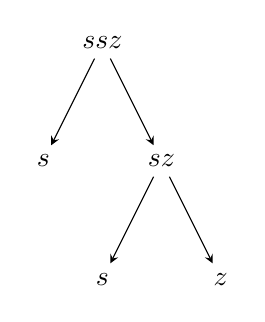
\begin{tikzpicture}[-stealth]
\node { $s\p{s\p{z}}$ }
  child { node { $s$ } }
  child { node { $s\p{z}$ }
    child { node { $s$ } }
    child { node { $z$ } }
  }
;
\end{tikzpicture}
\end{center}

As an example of what a construction tree interpretation of a function is good
for, we consider the important class of ``number-valued'' function algebras,
and prove by induction on the structure of a construction tree of a function $f
\in \mathcal{P}$, that $\mathcal{P}$ is number theoretic.

\begin{definition} A function algebra $\mathcal{F}$ is \textbf{number-valued}
if the codomain of every function $f \in \mathcal{F}$ is $\mathbb{N}$.
\end{definition}

\begin{theorem} \label{thm:p-number-valued} $\mathcal{P}$ is number-valued.
\end{theorem}

\begin{proof} By induction on the structure of a construction tree
$\mathcal{T}\p{f}$ of any $f\in \mathcal{P}$. There are two
cases:\begin{enumerate}[label=(\arabic*)]

\item $\mathcal{T}_\mathcal{P}\p{f}$ is a leaf, designating an initial function
$f \in \mathcal{P}_I$.

The zero and successor functions are trivially number-valued.

\item $\mathcal{T}_\mathcal{P}\p{f}$ is an internal node with outbound subtrees
$\mathcal{T}\p{g_1},\ldots,\mathcal{T}\p{g_n}$, designating the application of
an operation $o \in \mathcal{F}_O$ to the functions $g_1,\ldots,g_n$.

By IH, $g_1,\ldots,g_n$ are all number-valued. RTS $o\p{g_1,\ldots,g_n}$ is
number-valued. There is only one operation in $\mathcal{P}_O$: composition,
where $g_1$ is the \emph{composition operator}, and $g_2,\ldots,g_n$ are the
\emph{composition operands}. By \refDef{function-algebra-p}, the codomain of
the composite function is the codomain of the composition operator, which we
know is number-valued.\end{enumerate}\end{proof}

\refProof{p-number-valued} is an example of an important proof technique called
``structural induction'', which is useful for proving properties of, among
other things, function algebras.

% In the case of $\mathcal{P}$, the construction tree is unique. Otherwise,
% either there is an initial function which gives rise to multiple function in
% $\mathcal{F}$. which is clearly absurd.

% Such an interpretation gives another view of the initial functions as opposed
% to operators --- initial function do not depend on their values for smaller
% arguments --- no that's the nonrecursive functions.

The zero and successor functions, as well as the composition operation above
are perhaps ``unequivocally'' considered computable, but $\mathcal{P}$ also
gives rise to a fairly ``trivial'' set of functions. It has already been shown
that $\mathcal{P}$ is (merely) number-valued. Drastically more stringent
restrictions are proven below, using similar means.

\begin{lemma} \label{lem:p-tree-leafs} A construction tree
$\mathcal{T}_\mathcal{P}\p{f}$ has $x=i+j$ leafs, for some $x,i,j \in
\mathbb{N}$, $j$ of which are zero leafs, and $i$ of which are successor leafs.
\end{lemma}

\begin{proof} By \refDef{function-algebra-p} and \refDef{construction-tree},
every leaf of $\mathcal{T}_\mathcal{P}\p{f}$ is either a zero- or successor
leaf. Any finite tree has a $x=i+j$ leafs for some $x,i,j \in \mathbb{N}$.
WLOG, let $\mathcal{T}_\mathcal{P}\p{f}$ have $i$ zero leafs, and $j$ successor
leafs. \end{proof} 

This machinery is useful to questioning the role of zero leafs.

Consider the case with no zero leafs. That is, an $f \in \mathcal{P}$ is merely
some composition of successor functions, and so for any natural number $n$,
$f\p{n}=n+i$, where $i$ is the number of (successor) leafs in
$\mathcal{T}_\mathcal{P}\p{f}$. For instance, both $s\p{s\p{s}}$ and
$s\p{s}\p{s}$ yield the third successor of the input value. The two
construction trees are illustrated below:

\begin{center}
\begin{minipage}{0.4\textwidth}
\begin{center}
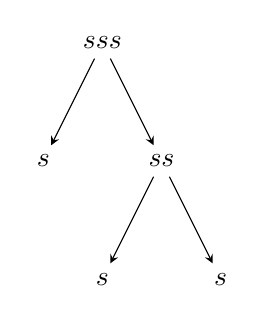
\begin{tikzpicture}[-stealth]
\node { $s\p{s\p{s}}$ }
  child { node { $s$ } }
  child { node { $s\p{s}$ }
    child { node { $s$ } }
    child { node { $s$ } }
  }
;
\end{tikzpicture}
\end{center}
\end{minipage}
%
\begin{minipage}{0.4\textwidth}
\begin{center}
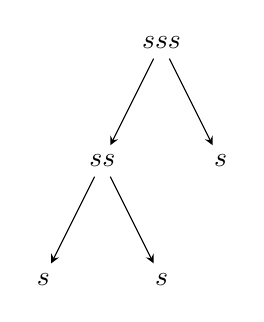
\begin{tikzpicture}[-stealth]
\node { $s\p{s}\p{s}$ }
  child { node { $s\p{s}$ }
    child { node { $s$ } }
    child { node { $s$ } }
  }
  child { node { $s$ } }
;
\end{tikzpicture}
\end{center}
\end{minipage}
\end{center}

\begin{lemma} \label{lem:p-no-zero} If $\mathcal{T}_\mathcal{P}\p{f}$ has $j=0$
zero leafs, and $i$ successor leafs, then $f : \mathbb{N} \rightarrow
\mathbb{N}$ and $f\p{n} = n + i$ for all $n \in \mathbb{N}$. \end{lemma}

\begin{proof} By induction on the structure of $\mathcal{T}_\mathcal{P}\p{f}$.
There are two cases:\begin{enumerate}[label=(\arabic*)]

\item $\mathcal{T}_\mathcal{P}\p{f}$ is a leaf. This must be a successor leaf.
The lemma follows by definition of the successor function, as we have $i = 1$.

\item $\mathcal{T}_\mathcal{P}\p{f}$ is an internal node with outbound subtrees
$\mathcal{T}_\mathcal{P}\p{g_1},\ldots,\mathcal{T}_\mathcal{P}\p{g_n}$,
designating the application of an operation $o \in \mathcal{F}_O$ to the
functions $g_1,\ldots,g_n$. This must be a composition node, and so $n=2$.

By IH, for all $1 \leq k \leq 2$, $g_k : \mathbb{N} \rightarrow \mathbb{N}$ and
$g_k\p{m} = m + i_k$, for all $m \in \mathbb{N}$, where
$\mathcal{T}_\mathcal{P}\p{g_k}$ has $j_k = 0$ zero leafs, and $i_k$ successor
leafs.

By definition of composition, $f : \mathbb{N} \rightarrow \mathbb{N}$, and
$f\p{m}=g_1\p{g_2\p{m}} = g_1\p{m + i_2} = m + i_2 + i_1 = m + \p{i_1 + i_2}$,
for all $m \in \mathbb{N}$.  By definition of construction trees, the number of
leafs in $\mathcal{T}_\mathcal{P}\p{f}$ is $\p{i_1 + j_1} + \p{i_2 + j_2} = i_1
+ i_2$, all of which are successor leafs.  The lemma
follows.\end{enumerate}\end{proof}

Consider now the case with at least one zero leaf. The case with exactly one
zero leaf has already been illustrated. The case with multiple zero leafs
illustrates the usefulness of the ubiquity of the zero function(s).

\begin{lemma} \label{lem:p-at-least-one-zero} If $\mathcal{T}_\mathcal{P}\p{f}$
has $j \geq 1$ zero leafs, and $i$ successor leafs, then $f : S \rightarrow
\mathbb{N}$, for some set $S$, and $f\p{s} \leq i$. \end{lemma}

\begin{proof} \end{proof}

\begin{theorem} A function $f \in \mathcal{P}$, has $i+j$ leafs, of which $j$
leafs are zero leafs, and $i$ leafs are successor leafs. Furthermore,
either\begin{enumerate}[label=(\arabic*)]

\item $f : \mathbb{N} \rightarrow \mathbb{N}$, and $f\p{n} = n+i$ for all $n
\in \mathbb{N}$; or

\item $f : S \rightarrow \mathbb{N}$, for some set $S$, and $f\p{s} \leq i$ for
all $s \in S$.

\end{enumerate}\end{theorem}

\begin{proof} Follows directly from \refLem{p-tree-leafs}, \refLem{p-no-zero},
and \refLem{p-at-least-one-zero}. \end{proof}

This is a fairly limited set of functions, but it does form the core of many
much more general function algebras, leading to the notion of function
hierarchies:

\begin{definition} A \textbf{function hierarchy} $\mathcal{H}$ is a finite
sequence of function classes, $\mathcal{C}_1, \ldots, \mathcal{C}_n$, such that
$\mathcal{C}_1 \subseteq \mathcal{C}_2 \subseteq \cdots \subseteq
\mathcal{C}_{n-1} \subseteq \mathcal{C}_n$. \end{definition}

To get off the ground, we introduce one more initial function: projection, and
one more operator: primitive recursion, leading to the outset of the so-called
Grzegorczyk hierarchy which will reappear in later chapters.

The uniqueness property can be relaxed if we let the composition operation be
transitive. That is, if we let\begin{align*}
%
\kappa^n_1\p{f,\kappa^n_1\p{g,h}} = \kappa^n_1\p{\kappa^n_1\p{f,g},h}
%
\quad \quad \text{or simply} \quad \quad
%
f\p{g\p{h}} = f\p{g}\p{h}
%
\end{align*}

\begin{tikzpicture}
\node { $s\p{s\p{z}}$ }
  child { node { $s\p{s}$ }
    child { node { $s$ } }
    child { node { $s$ } }
  }
  child { node { $z$ } }
;
\end{tikzpicture}

Note, in particular, that $s\p{s} \in \mathcal{P}$.

The functions above are perhaps ``unequivocally'' considered computable, but
also give rise only to a fairly ``trivial'' set of functions, adequate for
little more than the construction of natural number representations, one
subsequent natural number at a time.

% definition by = scheme

To get off the ground we need to employ the scheme of definition by recursion.
In a recursive scheme, a function is still given by a set of equations, but the
function being defined also appears on the right-hand side of the equality
sign.

Loops are not allowed in a construction tree.

Unfortunately, such a recursion does not terminate. A \emph{primitive} form of recursion 

Any construction tree is finite.

A function is defined by the scheme of primitive recursion over natural numbers
if it is given by the following recursion scheme: Without loss of generality,
consider defining a function $f : \mathbb{N} \times \mathbf{A} \rightarrow B$.
That is, let the first argument of $f$ (the recurrence argument) be a natural
number, with the remaining arguments (if any) forming an element of some set
$\mathbf{A}$, and let $f$ yield a value of some set $B$. $f$ is given by
primitive recursion from functions $g : \mathbf{A} \rightarrow B$ and $h :
\mathbb{N} \times \mathbf{A} \times B \rightarrow B$ if it satisfies the
following: \begin{align*}
%
f\p{0, \mathbf{y}} &= g\p{\mathbf{y}}\\
%
f\p{x+1, \mathbf{y}} &= h\p{x,\mathbf{y},f\p{x,\mathbf{y}}}
%
\end{align*}

We are now ready 

\todo{A \textbf{hierarchy of functions}, successively takes a class of
functions as initial functions and closes it under a set of operations.}

% That is, for all $f
%\in \mathcal{C}_I$, we have $f \in \mathcal{C}$, and for all $g \in \mathcal{C}_O$, 


% initial functions: the set of functions which form the leafs of a computation
% tree; it is however up to interepretation what one regards as the leafs of
% this computation tree, except for perhaps the 0-ary functions, which lead to
% no subsequent function calls. On the other hand, our definition of the
% successor function also leads to no 

% in classical recursion theory, we define functions over the natural numbers;
% we designate some functions as initial, and others as operators. The
% operators combine the initial functions and operators to construct new
% values. This induces a construction tree. Given sufficiently simple initial
% functions, and sufficiently simple constructions -- we can superimpose a
% computation model on top of a function algebra. Here, sufficiently simple
% means computable, and typically, easily computable.

\todo{One classical example of a function algebra is the Grzegorzcyk hierarchy.}

\section{Semantics}

Inspired by \cite{hofmann-2003}, we sometimes give the set-theoretic
denotational semantics of the operators in a programming language. To this end,
for every base type $A$, we assume a set $\sem{A}$, e.g. $\mathtt{N} =
\mathbb{N}$.

\section{Projection}

\label{sec:generalised-projection}

\begin{definition} Let $\mathtt{PROJ}_j : S_1 \times \cdots \times S_n
\rightarrow T$ be a \textbf{generalised projection} operator, having the
denotational semantics $\sem{\mathtt{PROJ}_j\p{x_1,\ldots,x_n}} = \sem{x_j}$,
for some $j,n \in \mathbb{N}$, such that $1 \leq j \leq n$.  \end{definition}

\begin{remark} $\mathtt{PROJ}_j$ is parametric in the types $S_1,\ldots,S_n$
and $T$. In simpler cases, we might let $S_1 = \cdots S_n = S$, and have
$\mathtt{PROJ}_j$ parametrized in $S$ and $T$. We may even let $S = T = A$, for
some given type $A$, written $\mathtt{PROJ}_j^A$, giving perhaps the more
comprehensible type, $\mathtt{PROJ}_j^A : A^n \rightarrow A$. \end{remark}

\begin{definition} Let $\mathtt{proj}_j$ be the operational interpretation of
$\mathtt{PROJ}_j$, having in particular, the following semantics:\begin{align*}
%
\axiom{ \mathtt{proj}_j\p{x_1,\ldots,x_{n}} \goesto x_j }
%
\end{align*}

\end{definition}

\section{Composition}

\label{sec:generalised-composition}

\begin{definition} Let $\mathtt{COMP}$ be a \textbf{composition} operator,
having the denotational semantics $\sem{\mathtt{COMP}\p{f,g_1,\ldots,g_m}} =
h$, for some $m,n\in \mathbb{N}$, where \begin{align*}
%
f & : T_1 \times \cdots \times T_m \rightarrow U \\
%
g_1 & : S_1 \times \cdots \times S_n \rightarrow T_1 \\
%
& \ldots \\
%
g_m & : S_1 \times \cdots \times S_n \rightarrow T_m \\
%
h & : S_1 \times \cdots \times S_n \rightarrow U.
%
\end{align*} $h$ itself is given as follows, where $\vect{x} \triangleq
x_1,\ldots,x_n$:\begin{align*}
%
h\p{\vect{x}} = \sem{f}\p{\sem{g_1}\p{\vect{x}}, \ldots,
\sem{g_m}\p{\vect{x}}}.
%
\end{align*}

\end{definition}

\begin{remark} $\mathtt{COMP}$ is parametric in the types $S_1,\ldots,S_n$,
$T_1,\ldots,T_m$, and $U$. In simpler cases, we might let $S_1 = \cdots = S_n =
S$, and let $T_1 = \cdots T_m = T$, and have $\mathtt{COMP}$ parametrized in
$S$, $T$, and $U$. We may even let $S=T=U=A$, for some given type $A$, written
$\mathtt{COMP}_A$, giving the more comprehensible type:\begin{align*}
%
\mathtt{COMP}_A : \p{A^m \rightarrow A} \rightarrow \p{A^n \rightarrow A}^m
\rightarrow A^n \rightarrow A.
%
\end{align*}\end{remark}

\begin{notation} $\mathtt{COMP}\p{f, \vect{g}}$, where $\vect{g} \triangleq
g_1,\ldots,g_m$, is also written as $f\p{\vect{g}}$. \end{notation}

\begin{definition} Let $\mathtt{comp}$ be the operational interpretation of
$\mathtt{COMP}$, having in particular, the following operational semantics,
where $\vect{x} \triangleq x_1, \ldots, x_n$:\begin{align*}
%
\judgement{
%
  g_1\p{\vect{x}} \goesto y_1 \quad \cdots \quad g_m\p{\vect{x}} \goesto y_m
\quad f\p{y_1,\ldots, y_m} \goesto z
%
}{
%
  \mathtt{comp}\p{f,g_1,\ldots,g_m}\p{\vect{x}} \goesto z
%
}
%
\end{align*}

\end{definition}

\section{Explicit Transformation}

\label{sec:explicit-transformation}

\begin{definition} \cite[p. 21]{smullyan-1961} Let $\mathtt{EXTR}$ be an
\textbf{explicit transformation} operator, having the semantics
$\sem{\mathtt{EXTR}\p{f,e_1,\ldots,e_m}} = h$, for some $m,n \in \mathbb{N}$,
where\begin{align*}
%
f & : S^m \rightarrow T \\
%
e_1, \ldots, e_m & : S + \set{1,\ldots,n} \\
%
h & : S^n \rightarrow S.
%
\end{align*} So each $\sem{e_i}$ is either some $s \in S$, or some $j \in
\set{1,\ldots, n}$. $h$ itself is given as follows:\begin{alignat*}{3}
%
h\p{x_1,\ldots,x_n} &= \sem{f}\p{g\p{\sem{e_1}},\ldots,g\p{\sem{e_m}}} \\
%
& & \text{where} \; g\p{\mathtt{inl} \; s} &= s \\
%
& & g\p{\mathtt{inr} \; j} &= x_j
%
\end{alignat*}

\end{definition}

\begin{remark} $\mathtt{EXTR}$ is parametric in the types $S$ and $T$. In
simpler cases, we might let $S=T=A$, for some given type $A$, written
$\mathtt{EXTR}_A$. \end{remark}

$\mathtt{EXTR}$ is a generalised substitution operator. Using $\mathtt{EXTR}$,
we can obtain not only $\mathtt{PROJ}$ and $\mathtt{COMP}$, but also various
permutation functions.  On the other hand, we can obtain $\sem{\mathtt{EXTR}}$
from $\sem{\mathtt{PROJ}}$, $\sem{\mathtt{COMP}}$, and the {\bfseries
\color{red} initial operators} \cite{rose-1984}. The theorem follows:

% Grzegorzcyk has multiple notions of substitution, maybe it is worthwhile to
% point out what "generalised substitution" really means.

\begin{theorem}\label{thm:extr-comp-proj} $\p{\Sigma,\set{\mathtt{EXTR}} \cup
O} = \p{\Sigma,\set{\mathtt{COMP}, \mathtt{PROJ}} \cup O}$. \end{theorem}

\begin{proof} \todo{Missing} \end{proof}

\section{Primitive Recursion}

\label{sec:primitive-recursion}

Motivated by \cite{leivant-1995}, we introduce a generalised form of primitive
recursion, also referred to as ``structural recursion''\cite{hofmann-2002}:

\index{recursion!primitive}
\index{recursion!structural|see {primitive recursion}}

\begin{definition} Let $\mathtt{PREC}$ be a \textbf{generalised primitive
recursion} operator over an inductively defined data type $S$, where
$s_1,\ldots,s_n$ are the value constructors of $S$, with the denotational
semantics $\sem{\mathtt{PREC}\p{g_{s_1},\ldots,g_{s_n}}} = f$ with the
type\begin{align*}
%
f : S \times T_1 \times \cdots \times T_k \rightarrow U
%
\end{align*}and defined as\begin{align*}
%
f\p{s_i\p{x_1,\ldots,x_m},y_1,\ldots,y_k} = \sem{g_{s_i}}\p{\vect{x}, \vect{y},
\vect{f}} & \quad \quad \p{\text{for all $i \in \set{1, \ldots, n}$}}
%
\end{align*} where

\begin{enumerate}

\item $\vect{x}$ is a subsequence of $x_1,\ldots,x_m$;

\item $\vect{y}$ is a subsequence of $y_1,\ldots,y_k$; and

\item $\vect{f}$ is a subsequence of $f\p{x_1, \vect{y}},\ldots, f\p{x_m,
\vect{y}}$.

\end{enumerate}

\end{definition}

In order to talk about primitive recursion, we also introduce the following
terminology:

\begin{itemize}

\item We say that the $s_i\p{x_1,\ldots,x_m}$ on the left hand side is the
\textbf{recurrence argument}, and $\vect{f}$ on the right hand side are
\textbf{critical arguments}.

\index{recurrence!argument}
\index{arguments!critical}

\item We als call the $g_{s_i}$'s above \textbf{recurrence functions}, where
$g_{s_i}$ is a \textbf{base function} if it takes no critical arguments, and is
a \textbf{step function} otherwise.

\index{recurrence!functions}
\index{functions!base|see {recurrence functions}}
\index{functions!step|see {recurrence functions}}

\item We say that the recurrence argument \textbf{drives} the recursion.

\index{recurrence!(drives a)}

\end{itemize}

\todo{All primitive recursions over inductive data types bottom out.}


\chapter{Bounded Primitive Recursion on Notation}

\begin{quotation}

\footnotesize\sffamily\itshape

\begin{flushright}

If one oversteps the bounds of moderation, \\
the greatest pleasures cease to please.

\smallbreak

\upshape

--- Epictetus, \emph{late Stoic philosopher} (55--135 A.D.)

\end{flushright}

\end{quotation}

Perhaps the most obvious way to characterise \FPTIME{}, is to explicitly bound
the function defined to take time at most polynomial in the size of the input,
without further reflections on how such a bound may be instated. Even at this
level, numerous questions arise:

\begin{enumerate}[label=(\arabic*)]

\item What is a good measure of size?

\item What are the necessary and sufficient means to state a bound like
``polynomial in the size of the input''?

\item What does a bounded function definition look like?

\end{enumerate}  

Such a general characterisation, taking a shot at the questions above, appeared
in the seminal conference paper \cite{cobham-1965}. Consequently, this paper
helped to establish computational complexity as a field\cite{clote-1999}.

The original characterisation was given recursion theoretically, in terms of a
function algebra over natural numbers. Cobham's choice of initial functions and
operations superimposed the use of a ``decimal notation'' of the natural
numbers. Given some further refinements of the operators, this gave   of the
function algebra superimposed the use of a decimal notation. Given the choice
of operators The following characterisation is equivalent up to choice of words
and notation:

\begin{definition}\cite{cobham-1965}

Let $s_i\p{x} = 10 \cdot x + i$ be a generalised successor function for

\end{definition}

The original characterisation was given in terms of a single-sorted word
signature, in particular, the natural numbers in decimal notation. The
following characterisation equivalent up to choice of words and notation,
except:

\begin{enumerate}[label=(\arabic*)]

\item we give the denotational rather than recursion-theoretic semantics of the
operators in a step towards a more operational characterisation.

\end{enumerate}

\def\smashf{\ensuremath{\mathtt{\#}}}
\def\cdotnot{\ensuremath{\cdot}}

\begin{definition} \cite{cobham-1965}

\begin{enumerate}[label=(\arabic*)]

\item Let $\mathtt{N}$ be a base type of natural numbers with $\sem{\mathtt{N}}
= \mathbb{N}$.

\item Let $\mathtt{0} : \mathtt{N}$ be a \textbf{constant} operator with
$\sem{\mathtt{0}} = 0$.

\item Let $\mathtt{s_0}, \ldots, \mathtt{s_9} : \mathtt{N} \rightarrow
\mathtt{N}$ be the $10$ \textbf{successor} operators, having the following
semantics:\begin{align*}
%
\sem{\mathtt{s_0}}\p{x} &= 10x + 0 \\
%
&\ldots \\
%
\sem{\mathtt{s_9}}\p{x} &= 10x + 9
%
\end{align*} In particular, $\sem{\mathtt{s_0}}\p{0} = 0$,
$\sem{\mathtt{s_0}}\p{1} = 10$, $\sem{\mathtt{s_5}}\p{0} = 5$,
$\sem{\mathtt{s_5}}\p{1} = 15$, etc. 

\item Let $\mathtt{COMP}$ be a \textbf{composition} operator, defined as in
\refSec{generalised-composition}, parametrised by the types $S=T=U=\mathtt{N}$.
That is, any occurrence of $\mathtt{COMP}$ has, for  some $m,n\in\mathbb{N}$,
the following type:\begin{align*}
%
\p{\mathtt{N}^m \rightarrow \mathtt{N}} \rightarrow \p{\mathtt{N}^n \rightarrow
\mathtt{N}}^m \rightarrow \mathtt{N}^n \rightarrow \mathtt{N}
%
\end{align*} In particular, both occurrences of $\mathtt{COMP}$ in
$\mathtt{COMP}\p{\mathtt{s_4}, \mathtt{COMP}\p{\mathtt{s_2}, \mathtt{z}}}$,
have the type $\p{\mathtt{N} \rightarrow \mathtt{N}} \rightarrow \mathtt{N}
\rightarrow \mathtt{N}$. Recall, that $\mathtt{COMP}\p{f,\vect{x}}$ is also
written as $f\p{\vect{x}}$, and so $\mathtt{COMP}\p{\mathtt{s_4},
\mathtt{COMP}\p{\mathtt{s_2}, \mathtt{z}}}$ is more concisely written as
$\mathtt{s_4}\p{\mathtt{s_2}\p{\mathtt{z}}}$.

\item Let $\mathtt{EXTR}$ be an \textbf{explicit transformation} operator,
defined as in \refSec{explicit-transformation}, parametrised by the types
$S=T=\mathtt{N}$.

\item Let $\sem{\mathtt{BPRN}}$ be a \textbf{bounded primitive recursion on
notation} operator, having the semantics
$\sem{\mathtt{BPRN}\p{g,h_0,\ldots,h_9,k}} = f$, for some $\sem{g} :
\mathbb{N}^n \rightarrow \mathbb{N}$, $\sem{h_0}, \ldots, \sem{h_9} :
\mathbb{N} \times \mathbb{N}^n \times \mathbb{N} \rightarrow \mathbb{N}$ and
$\sem{k} : \mathbb{N} \times \mathbb{N}^n \rightarrow \mathbb{N}$, where $f$
has type $\mathbb{N} \times \mathbb{N}^n \rightarrow \mathbb{N}$, and $f$ is
given by the following recursion scheme, where $\vect{y} =
y_1,\ldots,y_n$:\begin{align*}
%
f\p{\mathtt{s_0}\p{0}, \vect{y}} &= \sem{g}\p{\vect{y}} \\
%
f\p{\mathtt{s_0}\p{x}, \vect{y}} &= \sem{h_0}\p{x, \vect{y}, f\p{x, \vect{y}}}
& \text{if $x\neq 0$}\\
%
f\p{\mathtt{s_1}\p{x}, \vect{y}} &= \sem{h_1}\p{x, \vect{y}, f\p{x, \vect{y}}}
\\
%
&\cdots \\
%
f\p{\mathtt{s_9}\p{x}, \vect{y}} &= \sem{h_9}\p{x, \vect{y}, f\p{x, \vect{y}}}
\\
%
f\p{x, \vect{y}} &\leq \sem{k}\p{x, \vect{y}}
%
\end{align*} where $f$ itself has the following type:\begin{align*}
%
f : \mathbb{N} \rightarrow \mathbb{N}^n \rightarrow \mathbb{N}.
%
\end{align*}

Notably, given the denotational semantics of
$\mathtt{s_0},\ldots,\mathtt{s_9}$, any $n \in \mathbb{N}$ can be represented
as \begin{align*}
%
x_1\p{\cdots x_{\card{n}}\p{0} \cdots} & \quad \quad \text{where $x_i \in
\set{\mathtt{s_0}, \ldots, \mathtt{s_9}}$}
%
\end{align*}


\todo{this is to be interpreted as}

\item Let $\card{\mathrel{}\cdotnot\mathrel{}} : \mathbb{N} \rightarrow
\mathbb{N}$ be a \textbf{size function} such that $\card{x} =
\ceil{\log_{10}\p{x+1}}$.

\item Let $\sem{\cdotnot \; \smashf{} \; \cdotnot} : \mathbb{N} \times
\mathbb{N} \rightarrow \mathbb{N}$ be a \textbf{smash} operator, having the
semantics $\sem{x \smashf{} y} = \sem{x}^\card{\sem{y}}$.

\item Let $\mathcal{L} = \seq{s_i, \smashf{}, \mathtt{EXTR}, \mathtt{COMP},
\mathtt{BPRN}}$. That is, $\mathcal{L}$ is the smallest class of functions
containing the generalised successor and smash functions, \todo{closed under}
the operations of explicit transformation, composition, and bounded primitive
recursion on notation.

\end{enumerate}

\end{definition}

The detailed proofs that $\mathcal{L}$ is \FPTIME-sound and \FPTIME-complete,
appeared later in e.g.  \cite{rose-1984,clote-1999} using binary notation, and
in \cite{tourlakis-1984} using $n$-ary notation, for any $n>1$.  The proofs are
sketched below.

Firstly, going from decimal to binary, in general, to $n$-ary notation, the
size function must be adequately modified:

\begin{definition} \label{def:n-ary-notation} For $n$-ary notation, for any
$n>1$, and $x\geq 1$, let the \textbf{size function} be given as $\card{x} =
\ceil{\log_n\p{x+1}}$. As for the special cases, for $n=1$, let $\card{x}=x$,
and for $n=0$, let $\card{x}=0$. As a matter of covenience, note the
following:\begin{align*}
%
\ceil{\log_n\p{x+1}} \leq \log_n\p{x+1} + 1 \leq \log_n\p{x} + 2 =
\bigOh{\log_n\p{x}}.
%
\end{align*} \index{size function!$n$-ary notation} \end{definition}

Two other prominent changes are often done to the definition of $\mathcal{L}$
(see e.g. \cite{rose-1984, buss-phd-1985-6, bellantoni-cook-1992, clote-1999},
but somewhat surprisingly, not \cite{tourlakis-1984}):

\begin{enumerate}[label=(\arabic*)]

\item $\sem{\mathtt{EXTR}}$ is replaced by $\sem{\mathtt{PROJ}}$. In the
presence of $\sem{\mathtt{COMP}}$, by \refThm{extr-comp-proj}, this is
admissible.

\item For binary notation, the smash operator, is instead given with the
semantics $\sem{x \smashf{} y} = 2^{\card{\sem{x}} \cdot \card{\sem{y}}}$. Of
course, for binary notation, we have\begin{align*}
%
x^\card{y} = \p{2^{\log_2{x}}}^\card{y} \leq
\p{2^{\ceil{\log_2\p{x+1}}}}^\card{y} = \p{2^\card{x}}^\card{y} = 2^{\card{x}
\cdot \card{y}}.
%
\end{align*}So this too, is admissible\footnote{The diligent reader might find
it peculiar that \FPTIME{} is stable under small perturbations of ``smash'';
contrast the proofs in \cite{tourlakis-1984} and \cite{clote-1999}.}.

\end{enumerate}

The latter choice of smash operator is perhaps best motivated by the fact that,
for binary notation, for any \todo{monotone} polynomial $p$, we
have\begin{align*}
%
\log_2\p{2^{p\p{\card{x}}}} = p\p{\card{x}}
%
\quad \quad \text{and so} \quad \quad
%
\card{2^{p\p{\card{x}}}} = \bigOh{p\p{\card{x}}}
%
\end{align*} This admits perhaps a more natural construction of a value
\emph{polynomial in size} in the size of the input, i.e. a value of size
$p\p{\card{x}}$ for a given value of size $\card{x}$, for any monotone
polynomial $p$. In particular, with this notion of smash,\begin{align*}
%
\sem{\underbrace{x \smashf{} \cdots \smashf{} x}_{\text{$k$ times}}} =
2^{\card{\sem{x}}^k}
%
\quad\quad \text{and so} \quad\quad
%
\card{\sem{\underbrace{x \smashf{} \cdots \smashf{} x}_{\text{$k$ times}}}} =
\bigOh{\card{\sem{x}}^k}.
%
\end{align*} At the same time, for $n$-ary notation, where $n>1$, we
have\begin{align*}
%
\card{x^\card{y}} &= \bigOh{\log_n\p{x^\bigOh{\log_n\p{y}}}} \\
%
                  &= \bigOh{\log_n\p{x^{\log_n\p{y}}}} \\
%
                  &= \bigOh{\log_n\p{x} \cdot \log_n\p{y}} \\
%
                  &= \bigOh{\card{x} \cdot \card{y}}
%
\end{align*} So the two smash functions $x^\card{y}$ and $2^{\card{x} \cdot
\card{y}}$ yield values equivalent in size, up to (fairly small) constant
factors (see also \refDef{n-ary-notation}). $x^\card{y}$ however, is easier to
generalise to $n$-ary notation.

\begin{lemma} \label{lem:l-fptime-sound} $\mathcal{L}$ is \FPTIME{}-sound.
\end{lemma}

\begin{proof} (Sketch, see also \cite{rose-1984, tourlakis-1984, clote-1999}.)
Proof by simulation of $\mathcal{L}$ on an \FPTIME{} TM.  \todo{Rest of sketch
missing.} \end{proof}

\begin{lemma} \label{lem:l-fptime-complete} $\mathcal{L}$ is
\FPTIME{}-complete. \end{lemma}

\begin{proof} (Sketch, see also \cite{rose-1984, tourlakis-1984, clote-1999}.)
Proof by simulation of an \FPTIME{} TM in $\mathcal{L}$. Performing primitive
recursion on notation on $u$, we can simulate $p\p{\card{t}}$-time TM, by
simulating the transition function of the TM with the step function of the
primitive recursion.  \todo{Rest of sketch missing.} \end{proof}

\begin{theorem} \label{thm:l-captures-fptime} $\mathcal{L}$ captures \FPTIME{}.
\end{theorem}

\begin{proof} Follows directly from \refLem{l-fptime-sound} and
\refLem{l-fptime-complete}. \end{proof}

% Key to the \FPTIME{}-completeness of the characterisation in
% \cite{cobham-1965} is to permit the construction of a term polynomial in size
% in the size of the input term.  That is, given a term $t \in
% \mathcal{T}\p{\Psi}$, to construct a term $u \in \mathcal{T}\p{\Psi}$, such
% that $p\p{\card{t}} \leq \card{u}$, for some monotone polynomial

% $$p\p{x}=a_0 \cdot x^0 + a_1 \cdot x^1 + \cdots + a_k \cdot x^k,$$

% where $a_0$, $a_1$, \ldots, $a_k$ are non-negative constants. This permits to
% simulate a $p\p{\card{t}}$-time TM using primitive recursion on notation over
% $u$, by simulating a TM transition at every step of the recursion.

\begin{remark} The technique of simulating a bounded TM with primitive
recursion appeared perhaps for the first time in \cite[\textsection
10.2.1/176]{minsky-1967}.  \end{remark}

% \begin{definition} Let $\mathcal{T}_\downarrow\p{\Psi}$ denote the
% \textbf{ground terms} over $\Psi$. \end{definition}

% \begin{definition} Let $\mathcal{T}_\downarrow\p{\Psi}^{\leq i}$ denote the
%ground terms over $\Psi$ of size at most $i$, m.f.

% $$\mathcal{T}_\downarrow\p{\Psi}^{\leq i} = \set{ t \in
% \mathcal{T}_\downarrow\p{\Psi} \st{ \card{t} \leq i }}.$$

% \end{definition}

% We consider the total number of ground terms over $\Psi$ of size at most $i$,
% for any given $i \in \mathbb{N}$, written
% $\card{\mathcal{T}_\downarrow\p{\Psi}^{\leq i}}$.

% Intuitively, the ground terms $\mathcal{T}_\downarrow\p{\Psi}$ of a
% single-sorted word signature $\Psi$ with $m$ nullary symbols and $\p{n-m}$
% unary symbols form the nodes in a forest $\mathcal{F}_\downarrow\p{\Psi}$ of
% $m$ complete $\p{n-m}$-ary trees of unbounded height.

% The number of terms of size $i\in\mathbb{N}$ is the number of nodes of tree
% depth at most $i-1$ in $\mathcal{F}_\downarrow\p{\Psi}$. This is also the total
% number of nodes in $\mathcal{F}_\downarrow\p{\Psi}$, when the trees are bounded
% to height $i-1$, written $\mathcal{F}_\downarrow\p{\Psi}^{< i}$.

% \begin{theorem} For a single-sorted word signature $\Psi$, having no unary
% symbols, so $\p{n-m}=0$, e.g. the booleans, the number of ground terms of size
% $i>0$ is $m$, m.f.

% $$\card{\mathcal{T}_\downarrow\p{\Psi}^{\leq i}} = m \cdot \iverson{i>0}$$

% \end{theorem}

% \begin{proof} For any $i$, consider the forest
% $\mathcal{F}_\downarrow\p{\Psi}^{< i}$. If $i=0$, the forest has $0$ nodes.
% If $i>0$, the forest has exactly $m$ nodes. \end{proof} of the methods
% surveyed to conventional data types in general, in particular, 

% \begin{theorem} For a single-sorted word signature $\Psi$, having exactly one
% unary symbol, so $\p{n-m}=1$, e.g. the Peano naturals, we have

% $$\card{\mathcal{T}_\downarrow\p{\Psi}^{\leq i}} = m \cdot i$$

% \end{theorem}

% \begin{proof} For any $i$, consider the forest
% $\mathcal{F}_\downarrow\p{\Psi}^{< i}$. This is a forest of $m$ chains of
% length $i$. The number of nodes in such a chain is $i$.  \end{proof}

% \begin{theorem} For a single-sorted word signature $\Psi$, having more than one
% unary symbol, so $\p{n-m}>1$, e.g. binary notation, we have

% $$\card{\mathcal{T}_\downarrow\p{\Psi}^{\leq i}} = m \cdot
% \frac{\p{n-m}^i-1}{\p{n - m} - 1}$$

% \end{theorem}

% \begin{proof} For any $i$, consider the forest
% $\mathcal{F}_\downarrow\p{\Psi}^{< i}$. This is a forest of $m$ complete
% $\p{n-m}$-ary trees of height $i-1$. It is well-known that the number of
% nodes in such a tree is $\frac{\p{n-m}^i-1}{\p{n - m} -
% 1}$\cite{cormen-et-al-2009}.  \end{proof}

% \begin{example} $\card{\mathcal{T}_\downarrow\p{B}^{\leq i}} = 1 \cdot 2^i$.
% (Recall that we also count the empty string.) \end{example}

% \begin{definition} Let the size of a term over $\Sigma$ be the number of
% symbols involved in the construction of the term:

% \begin{align*}
% \card{v_0}        &=  0 \\
% \card{v_1\p{x}}   &=  \card{x} + 1 \\
%                  &   \vdots \\
% \card{v_{i}\p{x}} &=  \card{x} + 1
% \end{align*}

% \end{definition}

% To get a closed form for the size function, we make a simplifying assumption
% that there is at most 

% \begin{lemma} If $\Sigma$ is a single-sorted signature, then
% $\card{x}<\card{v_k\p{x}}$ for all $\p{i+1} \leq k \leq j$.  \end{lemma}

% \begin{definition} The \textbf{smash function} over a single-sorted word
% signature $\Psi$, with $m$ nullary and $\p{n-m}$ unary symbols, is a binary
% symbol \smashf{}, written in infix notation, with the property that $\card{x
% \smashf{} y} = {\card{x}\cdot\card{y}}$.\end{definition}

% The usefulness of the smash function is illustrated by the fact that $\card{x
% \smashf{} y} = 2^3$

% \begin{definition} A single-sorted word signature $\Sigma$, extended with a
% smash function is $\Sigma^\smashf{} \triangleq \Sigma \cup \set { \smashf{} : 2
% }$. \end{definition}

% In 1964 Cobham [C] gave the first recursion-theoretic characterization of
% polynomial time, using a recursion whose depth was the binary length of the
% number being recursed on, and using explicit polynomial bounds to control the
% size of the output.\cite{bellantoni-phd-1992}.

% recursion scheme over an inductively or coinductively defined data type (an
% algebra).

% \begin{remark} It seems a bit superfluous to deal in the additional argument
% vector $\vect{y}$ which we simply pass down to our base and step functions.
% This could be handled by e.g. partially applying $\vect{y}$ on the given
% functions.  Although not important to the recursion scheme, we will soon take
% the stance that the arguments in $\vect{y}$ are of a different ``nature'' than
% the arguments we recur on.\end{remark}

% It seems straight forward to generalize bounded primitive recursion on notation
% to many-sorted free algebras.

\section{Generalisation}

% There is nothing special about the choice of natural numbers in decimal
% notation: we can make due with a single-sorted word signature, i.e. the
% language of strings over an alphabet.

In element (1) of the definition of $\mathcal{L}$, we let $\sem{n} = n$, for
all $n \in \mathbb{N}$. This can be considered a matter of ``syntactic sugar'':
any $n \in \mathbb{N}$ (including $0$) can (also) be represented in
$\mathcal{L}$ as follows:\begin{align*}
%
x_1\p{\cdots x_{\card{n}}\p{0} \cdots} & \quad \quad \text{where $x_i \in
\set{\mathtt{s_0}, \ldots, \mathtt{s_9}}$}
%
\end{align*}

\todo{How do I deal with the fact that $\log_2\p{1} = 0$, so \card{0} = 0?}

It follows that if we introduce a \textbf{zero} operator $\sem{\mathtt{z}} :
\mathbb{N}$ with the semantics $\sem{\mathtt{z}} = 0$, we can do away with (1)
in the definition of $\mathcal{L}$.

This demands to a further change to the special cases of $\mathtt{BPRN}$, i.e.
those where $0$ occurs:\begin{align*}
%
f\p{\mathtt{s_0}\p{0}, \vect{y}} &= \sem{g}\p{\vect{y}} \\
%
f\p{\mathtt{s_0}\p{x}, \vect{y}} &= \sem{h_0}\p{x, \vect{y}, f\p{x, \vect{y}}}
& \text{if $x\neq 0$}
%
\end{align*} are replaced by \begin{align*}
%
f\p{\mathtt{z}, \vect{y}} &= \sem{g}\p{\vect{y}} \\
%
f\p{\mathtt{s_0}\p{\mathtt{z}}, \vect{y}} &= \sem{g}\p{\vect{y}} \\
%
f\p{\mathtt{s_0}\p{x}, \vect{y}} &= \sem{h_0}\p{x, \vect{y}, f\p{x, \vect{y}}}
& \text{if $x\neq \mathtt{z}$}
%
\end{align*}

Except for the bounding condition, $\mathtt{BPRN}$ now looks like a regular
structural recursion, as in \refSec{primitive-recursion}. Thus, we are dealing
with a \textbf{single-sorted word signature} $\Psi = \p{\mathbb{A},
\set{\mathtt{z}, \mathtt{s_0}, \ldots, \mathtt{s_9}}}$, of which $\mathbb{N}$
is merely a model.

Dealing in terms, rather than natural numbers, requires to modify the size
function e.g. to the length of the term, as in \refSec{size}. Changing the size
function, requires changing the smash function to conform to the general
rule:\begin{align*}
%
\card{x\smashf{}y} = \bigOh{\card{x} \cdot \card{y}}
%
\end{align*}

\todo{Give the generalised version of $\mathcal{L}$ and prove (not sketch)
\FPTIME{} capture.}

\section{Examples}

\todo{Missing}

Of course, it remains to prove that the bound indeed is satisfied, which
segways neatly into the following discussion.

\section{Discussion}

Although bounded primitive recursion on notation has led to some interesting
work \cite{cook-1975, buss-phd-1985-6, cook-urquhart-1993}, it is generally
discarded\cite{bellantoni-cook-1992}, based on either that:

\begin{enumerate}[label=(\arabic*)]

\item the smash operator is not ``small''; or

\item the bounds are enforced in an ``extensional'' manner, rather than being
an ``intensional'' property of the system.

\end{enumerate}

The first trouble is perhaps best delineated by \cite{cobham-1965} himself.
Neither $x^\card{y}$ for $n$-ary notation, nor $2^{\card{x} \cdot \card{y}}$
for binary notation, is in $\mathcal{E}^2$, i.e. the second level of the
so-called Grzegorczyk hierarchy\cite{grzegorczyk-1953}. Specifically,
$\mathcal{E}^2$ is \todo{the smallest class of functions over $n$-ary notation,
containing multiplication}, and closed under the operations of explicit
transformation, composition and bounded primitive recursion. In other words, we
cannot smash in linear space, that is, using an $O\p{\card{x}+\card{y}}$-space
Turing machine\cite{ritchie-1963}. On the other hand, \cite{buss-phd-1985-6}
finds the use of \smashf{} ``natural and elegant'', as it has precisely the
growth rate necessary to fund the \todo{polynomial-time hierarchy}.

As to the other trouble, to put a $\mathtt{BPRN}$ operator to good use, we need
to prove that the bounding inequality is satisfied.  This leads to grave
complications in the cited work, but is sometimes outwitted (see e.g.
\cite{cook-urquhart-1993}) by changing the semantics of $\mathtt{BPRN}$ to
simply cut off at overflow. This is perhaps indifferent to a classical
characterisation of \FPTIME{}.

Considering the techniques one might employ for proving such a bound, one
quickly finds oneself counting and guessing, rather than the bound being
``guaranteed by construction''.  It is perhaps this quality that makes bounded
primitive recursion on notation inherently ``inintrinsic'', rather than the
mere fact that the bounds are stated explicitly, as criticised by e.g.
\cite{hofmann-2000a}.


\chapter{Predicative Recursion}

\begin{quotation}

\footnotesize\sffamily\itshape

\begin{flushright}

What's in a name? that which we call a rose \\
By any other name would smell as sweet;

\smallbreak

\upshape

--- WILLIAM SHAKESPEARE, \emph{Romeo and Juliet}, Act II, Scene II

\end{flushright}

\end{quotation}

That which we call ``predicative'' recursion is also referred to as
``tiered''\cite{leivant-1990}, ``stratified''\cite{leivant-1993}, or
``ramified''\cite{leivant-1995} recursion. (The conflation of these terms
appears prevalent in mathematics.) Our motivation is due to
\cite{hofmann-2000a}, categorising in this fell swoop, both the seminal works
\cite{bellantoni-cook-1992} and \cite{leivant-1995}. Hofmann was in turn
motivated by \cite{bellantoni-phd-1992}.

The use of the term ``predicative'' itself is due to \cite{russell-1907}, who
suggested a ``predicative'' theory of sets to deal with the plaguing paradoxes
in na\"ive set theory, e.g. Russell's or liar paradox. Informally, the
definition of an entity is ``impredicative''\cite{goedel-1944}, if it refers
(directly, or indirectly) to a totality to which the entity being defined
itself belongs.  Many recursive definitions fall squarely into such totalities. 

\todo{It is forbidden to do recursion on a critical argument, i.e.
specifically, the result of a self-recursive call.}

The refinement due in this section is based on the idea that the values we
recur on in a recursive definition are of a ``different nature'' from the
rest\cite{caseiro-1996}. Consequently, a segregation of values must commence.
\todo{Segregation is done on the input values. Distinction between two-tiered
and many-tiered recursion (and mu measure?). See also \cite{leivant-1995}.}

% Two classical examples of an impredicative definition gone rogue are
% Russell's and the Liar paradoxes: 

% \begin{description}

% \item [Russell's paradox] Define the set $R$ to be the set of all sets which
% are not members of themselves. If $R$ is a member of itself, then it should
% not be a member of itself; if it is not a member of itself, then it should be
% a member of itself. Paradox by indirect self-reference.

% \item [Liar paradox] Define the liar sentence ``This sentence is false.'' If
% the sentence is true, then it is false; if it is false, then it is true.
% Paradox by direct self-reference.

% \end{description} 

\subsection{Two-tiered recursion}

Two-tiered recursion, also referred to as ``safe'' or ``controlled'' recursion,
was independently introduced in \cite{simmons-1988}, \cite{leivant-1990}, and
\cite{bellantoni-cook-1992}, and generally attributed to the latter.

The idea, as indicated above, is to segregate the values into ``normal'' and
``safe'' values. The normal values are assumed known in their totality. The
safe values are those (perhaps) obtained by impredicative means, i.e. via
recursion\cite{bellantoni-cook-1992, clote-1999}. Safely, as in, without
exceeding \FPTIME{}.

The variables are segregated purely syntactically, e.g. using a semicolon. In
particular, if $f$ is an $m+n$-ary symbol, with $m$ normal inputs and $n$ safe
inputs, it is written as $f\p{x_1,\ldots,x_m \semic{} x_{m+1},\ldots,x_{m+n}}$,
where $x_1,\ldots,x_m$ are the $m$ normal inputs, and $x_{m+1},\ldots,x_{m+n}$
are the $n$ safe inputs. If the eloquent programmer finds the explicit
segregation ineloquent, the segregation can be inferred from how the values
$x_1,\ldots,x_n$ are used\cite{caseiro-1996}.

The characterisation in \cite{bellantoni-cook-1992} is again given in terms of
a single-sorted word signature, in particular, the natural numbers in binary
notation. We give a characterisation equivalent up to choice of words and
notation, except that

\begin{enumerate}[label=(\arabic*)]

\item we give a (syntax-directed) operational semantics of the operators to
emphasise the syntactic nature of the characterisation; and

\item we make the distinction between normal and safe inputs explicit in the
type system, as suggested in \cite[\textsection\ 5]{bellantoni-cook-1992}.

\end{enumerate}

\begin{definition} \cite{bellantoni-cook-1992}

\begin{enumerate}[label=(\arabic*)]

\item Let $\mathbb{N}$ and $\Box\mathbb{N}$ denote the normal and safe data
types, respectively.

\item Let $\mathtt{z} : \Box\mathbb{N}$ be a \textbf{constant} operator, having
the following semantics:$$
%
\axiom{ \mathtt{z} \goesto \repr{0} }
%
$$

\item Let $\mathtt{s}_0,\mathtt{s}_1 : \Box\mathbb{N} \rightarrow
\Box\mathbb{N}$ be (binary) \textbf{successor} operators, having the following
semantics:$$
%
\judgement{ a \goesto \repr{n} }{
%
  \mathtt{s}_0\p{\semic{} a} \goesto \repr{2n}
%
} \quad
%
\judgement{ a \goesto \repr{n} }{
%
  \mathtt{s}_1\p{\semic{} a} \goesto \repr{2n + 1}
%
}
%
$$

\item Let $\mathtt{p} : \Box\mathbb{N} \rightarrow \Box\mathbb{N}$ be a
(binary) \textbf{predecessor} operator, having the following semantics: $$
%
\axiom{
%
  \mathtt{p}\p{\semic{} \mathtt{z}} \goesto \repr{0}
%
}
%
\quad\axiom{
%
  \mathtt{p}\p{\semic{} \mathtt{s}_i\p{\semic{} a}} \goesto a
%
}\p{\text{for $i \in \set{0,1}$}}
%
$$

\item Let $\pi_j : \mathbb{N}^m \times \Box\mathbb{N}^n \rightarrow
\Box\mathbb{N}$ be a generalised (safe) \textbf{projection} operator, for all
$1 \leq j \leq m+n$, given by the following semantics:$$
%
\axiom{ \pi_j\p{x_1,\ldots,x_m \semic{} x_{m+1},\ldots,x_{m+n}} \goesto x_j }
%
$$

Note, in particular, $\pi_j$ projects the input safe, and so $\pi_j$ is
\emph{not} a mere operational interpretation of the generalised projection
operator $\sem{\mathtt{PROJ}_j}$.

\item Let $\mathtt{cond} : \Box\mathbb{N} \times \Box\mathbb{N} \times
\Box\mathbb{N} \rightarrow \Box\mathbb{N}$ be a (safe) \textbf{conditional}
operator, having the following semantics:$$
%
\judgement{
%
  a \goesto \repr{n} \quad b \goesto m
%
}{
%
  \mathtt{cond}\p{\semic{} a, b, c} \goesto m
%
}\p{n \bmod 2 = 0}
%
\quad\judgement{
%
  a \goesto \repr{n} \quad c \goesto m
%
}{
%
  \mathtt{cond}\p{\semic{} a, b, c} \goesto m
%
}\p{n \bmod 2 \neq 0}
%
$$

\item Let $\mathtt{sprn}$ be a \textbf{safe primitive recursion on notation}
operator, having the following semantics, where $f \triangleq
\mathtt{sprn}\p{g, h_0, h_1}$:\begin{align*}
%
\judgement{
%
  g\p{\vect{y} \semic{} \vect{a}} \goesto c
%
}{
%
  f\p{\mathtt{z}, \vect{y} \semic{} \vect{a}} \goesto c
%
}\end{align*}\begin{align*}
%
\judgement{
%
  h_i\p{x, \vect{y} \semic{} \vect{a}, f\p{x,\vect{y} \semic{} \vect{a}}}
\goesto c
%
}{
%
  f\p{\mathtt{s}_i\p{x}, \vect{y} \semic{} \vect{a}} \goesto c
%
}\p{\text{for $i\in\set{0,1}$}}
%
\end{align*}

\item For every $f : \mathbb{N}^n \rightarrow \Box\mathbb{N}$, where $n \in
\mathbb{N}$, there is a corresponding $g : \mathbb{N}^n \rightarrow
\mathbb{N}$, in accordance with the following axiom:\begin{align*}
%
\axiom{f\p{x_1,\ldots,x_n} \goesto g\p{x_1,\ldots,x_n}}
%
\end{align*}

This permits the coersion of safe outputs to normal outputs.

\item Let $\mathcal{B} = \p{\set{\mathtt{s}_0, \mathtt{s}_1, \mathtt{p}, \pi_j,
\mathtt{cond}},\set{\mathtt{comp}, \mathtt{sprn}}} $, where $\mathtt{comp}$ is
defined as in \refSec{generalised-composition}, with $S=\mathbb{N}$ and
$T=U=\Box\mathbb{N}$.

\end{enumerate}

\end{definition}

\begin{remark} The size function is defined as before. In particular, for
binary notation, $\card{n}=\ceil{\log_2\p{n+1}}$ for all $n \in \mathbb{N}$.
\end{remark}

\begin{lemma} \label{lem:b-fptime-sound} $\mathcal{B}$ is \FPTIME{}-sound.
\end{lemma}

\begin{proof} (Sketch, see also \cite{bellantoni-cook-1992}.) By simulating
$\mathcal{B}$ in $\mathcal{L}$.  \todo{Rest of sketch missing.} \end{proof}

\begin{lemma} \label{lem:b-fptime-complete} $\mathcal{B}$ is
\FPTIME{}-complete.  \end{lemma}

\begin{proof} (Sketch, see also \cite{bellantoni-cook-1992}.) By simulating
$\mathcal{L}$ in $\mathcal{B}$. \todo{Rest of sketch missing.} \end{proof}

\begin{theorem} $\mathcal{B}$ captures \FPTIME{}. \end{theorem}

\begin{proof} Follows directly from \refLem{b-fptime-sound} and
\refLem{b-fptime-complete}. \end{proof}

\subsubsection{Example}

\subsubsection{Discussion}

\subsubsection{$\mu$-measure}

Before we turn to many-tiered recursion..

\subsection{Many-tiered recursion}

The generalization of two-tiered recursion to many-tiered recursion is
generally attributed to \cite{leivant-1995}. The intuition is that inputs come
bearing varying computational weights --- some are too heavy to drive a
recurrence.

In the style of \cite{leivant-1990}, the motivation for this work is to give an
algebraic, rather than a numeric, account of tiered recursion, drawing
parallels to programming with algebraic data types. As a ``technical
advantage'', the work also boasts an implicit characterisation of
$O\p{n^k}$-\TIME{} for any given $k\in \mathbb{N}$. This is considered useful
to Part II.

The characterisation in \cite{leivant-1995} is given in terms of free algebras.
The proofs of capture are given, ``without loss of generality'', in terms of
word algebras. Unfortunately, the means of proof do not generalise to tree
algebras\cite{caseiro-1996, dal-lago-et-al-2010}.

The conference paper \cite{dal-lago-et-al-2010} presents an alternative proof,
generalising tiered recursion to single-sorted free algebras. Their
characterisation is given below, equivalent up to choice of words and notation,
except:

\begin{enumerate}[label=(\arabic*)]

\item we give a (syntax-directed) operational semantics of the oprators to
emphasise the syntactic nature of the characterisation;

\item we let the tiers be a part of the type system rather than they stand on
their own, in leau of what we did for two-tiered recursion; and

\item we present the characterisation in terms of a many-sorted, rather than a
single-sorted signature, in leau of the above, and generalising slightly.

\end{enumerate}

\begin{definition} \cite{dal-lago-et-al-2010}

\begin{enumerate}[label=(\arabic*)]

\item Let $\Sigma$ be a many-sorted signature, decorated with tiers, and let
$\sigma : \Sigma \rightarrow \mathbb{N}$ give the arities of the symbols in
$\Sigma$.

\todo{A type signature?}

\item Let $s : S_1^i \times \cdots \times S_n^i \rightarrow T^i$ be the type of
any symbol $s \in \Sigma$. That is, the constructors of the algebra operate on
same-tier inputs, and preserve tier.

\item Let $\mathtt{proj}_j$ be a generalised projection operator, as in
\refSec{generalised-projection},  parametrised by the types $S_1^{i_1}, \ldots,
S_n^{i_n}$, and $S_j^{i_j}$, where $1 \leq j \leq n$.

\item Let $\mathtt{comp}_j$ be a generalised composition operator, as in
\refSec{generalised-composition}, parametrised by the types $S_1^{i_1}, \ldots,
S_n^{i_n}$, $T_1^{j_1}, \ldots, T_m^{j_m}$, and $U^k$.

Note, in particular, that for any $f : V^0 \rightarrow V^1$ and $g : V^0
\rightarrow V^0$, $\mathtt{comp}\p{f,g}$ is well-typed, whereas
$\mathtt{comp}\p{g,f}$ is not.

\item Let $\mathtt{trec}$ be a \textbf{tiered primitive recursion} operator,
having the following semantics: \begin{align*}
%
f \triangleq \mathtt{trec}\p{g_1,\ldots,g_m} \quad\quad
%
\vect{x} \triangleq x_1, \ldots, x_{\sigma\p{s_k}} \quad\quad
%
\vect{y} \triangleq y_1, \ldots, y_n \\
%
\judgement{
%
  g_l\p{\vect{x}, \vect{y}, f\p{x_1, \vect{y}}, \ldots, f\p{x_{\sigma\p{s_k}},
\vect{y}}} \goesto z
%
}{
%
  f\p{s_l\p{\vect{x}},\vect{y}} \goesto z
%
}\p{\text{for $k \in \set{1,\ldots,m}$}}
%
\end{align*} where, for $i<j$, the types are as follows, having $\mathbf{T}
\triangleq T_1^{k_1} \times \cdots \times T_n^{k_n}$:\begin{align*}
%
f &: S^j \times \mathbf{T} \rightarrow U^i \\
%
g_k &:  S_1^j \times \cdots \times S_{\sigma\p{s_l}}^j \times \mathbf{T} \times
\underbrace{U^i \times \cdots \times U^i}_{\text{$\sigma\p{s_l}$ times}}
\rightarrow U^i
%
\end{align*}

The key point with $\mathtt{trec}$ is that the tier of the value we recur on,
must be strictly greater than the tier of the value we produce with
$\mathtt{trec}$ ($i < j$).

\end{enumerate}

\end{definition}

The notable change with the tiered primitive recursion operator
($\mathtt{trec}$), in contrast to the previously introduced bounded primitive
recursion operator ($\mathtt{BPRN}$), and safe primitive recursion operator
($\mathtt{sprn}$), is that $\mathtt{trec}$ makes multiple recursive calls ---
once for each $x_i$ in $s_i\p{x_1,\ldots,x_n}$.

This streamlines the operational semantics, and does originally appear in
\cite{leivant-1995}. However, the paper goes on to prove the capture of
polynomial complexities in terms of word algebras only, i.e. where $\sigma\p{s}
\leq 1$ for every symbol $s$.

\begin{definition} A \textbf{single-sorted} algebra is an algebra over the
signature $\p{\set{B}, \mathcal{T}, \mathcal{V}}$, i.e. there is just a single
base type, $B$. \end{definition}

\begin{definition} A \textbf{word} algebra is an algebra over the signature
$\p{\mathbf{B}, \set{\rightarrow}, \mathcal{V}}$, where each $v \in
\mathcal{V}$ either has the kind $v : *$ or $v : *\rightarrow *$.
\end{definition}

\begin{example} A single-sorted word algebra is an algebra over the signature
$\p{\set{B},\set{\rightarrow}, \mathcal{V}}$, where for each $v \in
\mathcal{V}$ we either have $v : B$ or $v : B\rightarrow B$. \end{example}

\begin{definition} A \textbf{Peano numbers} algebra is a single-sorted word
algebra over the signature $\p{\set{N}, \set{\rightarrow},\set{\mathtt{0} : N,
\mathtt{s} : N \rightarrow N}}$. \end{definition}


This is sufficient to deal in all finite types and string types, e.g.  the
peano numbers or binary strings. Making our way towards mixed data types and
tuples, \cite{marion-2003} generalised tiered recursion to simple algebras.

\begin{definition} A \textbf{simple algebra} is an algebra over the signature
$\p{\mathbf{B}, \set{\rightarrow}, \mathcal{C}}$, where each value constructor
$c \in \mathcal{C}$ has the type $\tau_1 \rightarrow \tau_2 \rightarrow \cdots
\rightarrow \tau_n \rightarrow \tau$, for some $n\in \mathbb{N}$, such that
$\tau$ occurs at most once amongst the $\tau_i$.  \end{definition}

If we curry our eyes a bit, we can see how this leads way to ``simple'' tuples.
Indeed, \cite{marion-2003} employs the more concise notation
$\p{\tau_1,\tau_2,\cdots,\tau_n}\rightarrow \tau$ instead.  Although this
admits a slightly more eloquent class of data types, we need more ``complex''
tuples to even model good old trees.

Worse yet, the results in \cite{leivant-1995} rely on a size function where the
size of a term is the ``height of the parse-tree'' of the term. Leading to the
plausible deniability that tiered recursion still captures $\mathtt{FPTIME}$
when defined over any free algebra\cite{caseiro-1996}.

The generalization to \emph{any} free algebra comes about in
\cite{dal-lago-et-al-2010}. Their insight is that there is no need to copy (or
recompute) a value if it appears more than once in a term --- we could just
\emph{refer} to the same value. In a programming language without destructive
assignment, this is perhaps a natural optimization technique. Hence ``trees''
are really represented as graphs.

\begin{remark} With this generalisation we move away from the conventional
notion of the \emph{length} of a term $t$ being the cumulative number of
occurrences of symbols and variables in $t$, as in first-order term
rewriting\cite{klop-vrijer-2003}. \end{remark}

\begin{example} \cite{dal-lago-et-al-2003} Consider a program $\p{\p{\p{N,T}, N
\cup T, \set{z : N, s : N \rightarrow N, \mathtt{leaf} : T, \mathtt{node} : T
\times T \rightarrow T}}, \set{f}}$, where $f$ is given by the following set of
clauses:

\begin{align}
f\p{\symb{z}}       &\leadsto \symb{leaf} \\
f\p{\symb{s}\p{w}}  &\leadsto \symb{node}\p{f\p{w}, f\p{w}}
\end{align}

\end{example}


\chapter{Non-Size Increasing Computation}

\begin{quotation}

\footnotesize\sffamily\itshape

\begin{flushright}

there is a relationship between the absence and presence of successor-like
functions and the computational complexity of programs

\smallbreak

\upshape

--- \cite{jones-kristiansen-2009}

\end{flushright}

\end{quotation}

Although it might seem due to name this section ``Impredicative Recursion'', it
is perhaps too general a name for this section to end up concise. Besides,
drawing such a cleavage might charm us in the wrong direction.

Some impredicative definitions cause us trouble --- but certainly not all.  In
a similar vein, a purely ``predicative'' theory of sets did not catch on
either, in lieu of softer restrictions one could impose on set comprehension
(for more, see \cite{feferman-1964}). An adequate choice of axioms for a theory
of sets, remains a context-dependent question.

An early investigation into when impredicative recursion causes trouble is
perhaps due to \cite{caseiro-1996}. She notes that ``the real problem [...] is
not that [...] recurs on its input, but that [...] \emph{doubles} its input''.
This leads to the development of a technique she calls ``Don't Double
Criticals'' (DDC), where the critical arguments are inferred automatically, and
the recurrence function is \emph{semantically} prohibited in doubling the
result of a recursive call. A proof that DDC captures \FPTIME{} does appear in
\cite{caseiro-1996}, but the work was never published. Instead, in its attempt
to ``investigate how to treat critical arguments linearly'', it has inspired
the many works of others \cite{bellantoni-et-al-2000,
aehlig-schwichtenberg-2002, hofmann-2003}.

At roughly the same time, \cite[\textsection~24]{jones-1997}, characterised
\PTIME{} using first-order read-only programs. The characterisation was later
published in \cite{jones-1999}, and extended to arbitrary finite data orders
and tail-recursive programs in \cite{jones-2001}. The divergent paths later
conflate in e.g. \cite{hofmann-2002}, as it uses an important proof technique
of \cite{jones-2001}.

The work we focus on here is \cite{aehlig-schwichtenberg-2002}, which is
considered an alternate take on the results of \cite{hofmann-2003}.

\begin{definition} Let $\NSIFPTIME{}$ be the class of those functions $f \in
\FPTIME{}$, where $f : A \rightarrow B$, for which $\card{f\p{a}} \leq
\card{a}$ for all $a \in A$. That is, the output of the function is no greater
in size than the input of the function. \end{definition}

\subsection{Discussion}

The insights of Caseiro et al., also led to a generalisation of the results of
\cite{marion-2003} in the conference paper \cite{marion-moyen-2000}. In both,
the authors deal in simple algebras, i.e.  algebras with types $\sigma_1 \times
\cdots \times \sigma_n \rightarrow \sigma$, where each $\sigma_i$ occurs at
most once among $\sigma_1 \times \cdots \times \sigma_n$ (so a tree algebra is
not a simple algebra). \todo{The conference paper captures \FPTIME{} with a
semantic argument, and shows that $\proc{LCS}$ and $\proc{Insertion-Sort}$ are
representable in the system.} The results never made it past the conference,
perhaps due to the use of simple algebras, in lieu of the more general results
of e.g.  \cite{aehlig-schwichtenberg-2002} and \cite{hofmann-2003}.

\section{BCK-algebra}

\section{Examples}

\section{Discussion}


\chapter{Discussion}

\begin{quotation}

\footnotesize\sffamily\itshape

\begin{flushright}

The abuse of structural rules may have damaging complexity effects.

\smallbreak

\upshape

--- Jean-Yves Girard, {\itshape Light Linear Logic} (1998)

\end{flushright}

\end{quotation}

An in-depth discussion (and perhaps, generalisation) is missing for at least
two major approaches to implicitly characterising (sub)polynomial bounds:

\begin{enumerate}[label=(\arabic*)]

\item Polynomially-Bounded Values, as in \cite{niggl-wunderlich-2006} and
\cite{jones-kristiansen-2009}.

\item Bounded Linear Logic, as in \cite{girard-scedorov-scott-1992} and
\cite{dal-lago-hofmann-2010}.

\end{enumerate}

Arguably, these are perhaps the approaches closest to our onset of looking for
ways to characterise subpolynomial bounds.


\chapter{\PTIME{} and \FPTIME{}}

\begin{quotation}

\footnotesize\sffamily\itshape

\begin{flushright}

there is a relationship between the absence and presence of successor-like
functions and the computational complexity of programs

\smallbreak

\upshape

--- \cite{jones-kristiansen-2009}

\end{flushright}

\end{quotation}

\begin{quotation}

\footnotesize\sffamily\itshape

\begin{flushright}

{\upshape PETER HILTON} \\
Christ!! What happens now?!\\
{\upshape ALAN TURING} \\
It should tell use the day's Enigma settings!\\
{\upshape HUGH ALEXANDER} \\
How long!?!

\smallbreak

\upshape

--- Graham More, The Imitaiton Game (2014)

\end{flushright}

\end{quotation}


The fundamental insight highlighted by the above quotation underpins much work
done in \cite{jones-1999, jones-2001, kristiansen-voda-2005, hofmann-2003,
kristiansen-2008}, and of course, \cite{jones-kristiansen-2009}, among others.
We draw on this insight in a fundamental and perhaps extreme way, by taking the
notion of ``successor-like function'' to roughly mean ``enumerator'', and
consider the presence and absence of both particular successor-like \emph{and}
predecessor-like functions.

Implicit characterizations of complexity classes, e.g. PTIME, often start out
by considering first-order programs on natural numbers. That is, the
computation of (mathematical) functions of type $\mathbb{N} \rightarrow
\mathbb{N}$. (For a counterexample, see \cite{hofmann-2003}.) 

In lieu of \refThm{tm-total}, such results apply even if we replace
$\mathbb{N}$ (on either side) by any countable or countably infinite set. That
is, the results still hold even if we turn to the computation of (mathematical)
functions of type $A \rightarrow B$ for some countable or countably infinite
sets $A$ and $B$.

Crucially, \refThm{tm-total} relies on \emph{mathematical} functions, not
real-world transformations. Realistically, all we get is this: assuming that we
have a representation of a value of type $A$ as a natural number, we can
compute a natural number representation of the corresponding value of type $B$,
within the characterised bounds.

This outset of ``first-order programs on natural numbers'' ignores the
real-life hurdle of dealing with \emph{data structures} rather than natural
numbers. So such an exposition is arguably impractical, or more dramatically,
ignores certain \emph{complexities} involved in dealing with data.

Instead, we formalise a notion of ``successor'' and ``predecessor'', and
present seminal results in the characterisation of PTIME in terms of this
general framework. Informally, a successor or predecessor is any operation that
may change the size of any value in the program (including time?). In practice,
essentially any conceivable operation, except perhaps stalling.

\section{Programs}

% Many high-level programming languages have data types, and these data types
% cannot be coerced.

In the interest of capturing a wide range of programming paradigms in one
discussion, we give only a general specification of what we deem a program to
be. This specification will later be specialized for more concrete purposes. We
make no claim however, that in so doing, we capture all conceivable programming
paradigms.

\begin{specification}

A \textbf{program} $P = \p{P_\mathbf{D}, P_\mathbf{F}}$ is a finite set of
\textbf{data types} $P_\mathbf{D}$, and a finite set of \textbf{functions}
$P_\mathbf{F}$, subject to the following laws:

\begin{enumerate}

\item [P-1] Every data type $A \in P_\mathbf{D}$ forms a set.

\item [P-2] Every function $f \in P_\mathbf{F}$ computes a partial function $f
: A \rightharpoonup B$, for some $A, B\in P_\mathbf{D}$. We write $f : A
\rightharpoonup B \in P_\mathbf{F}$.

\item [P-3] For every data type $A \in P_\mathbf{D}$ there is a \textbf{size
function} $\card{\cdot} : A \rightarrow \mathbb{N}$, so for every $a \in A$ we
have $\card{a} \in \mathbb{N}$.

\end{enumerate}

\end{specification}

\begin{remark} We do not require that a function $f \in P_\mathbf{F}$ can
compute a partial function $f : A \rightharpoonup B$ between \emph{any} given
data types $A, B \in P_\mathbf{D}$, merely that it is a partial function
between \emph{some} given data types $A, B \in P_\mathbf{D}$.  \end{remark}

\begin{remark} The purpose of the size function is primarily semantic, and so
it need not be in $P_\mathbf{F}$, but of course, it could be. \end{remark}

\subsection{Successors and Predecessors}

\begin{definition} A partial function $s : X \rightharpoonup Y \in
P_\mathbf{F}$ is a \textbf{successor function} for some $x \in X$ iff $s\p{x}$
is defined and $\card{x} < \card{s\p{x}}$. \end{definition}

\begin{definition} A partial function $p : X \rightharpoonup Y \in
P_\mathbf{F}$ is a \textbf{predecesor function} for some $x \in X$ iff $p\p{x}$
is defined and $\card{p\p{x}} < \card{x}$. \end{definition}

That is, a successor function produces an output \emph{strictly greater} in
size than its input, and a predecessor function produces an output
\emph{strictly lesser} in size than its input.

Note in particular, that whether a given partial function $f : X
\rightharpoonup Y \in P_\mathbf{F}$ is a successor or predecessor function, if
either, \emph{depends} on the value $x \in X$ which $f$ is applied to. If $X$
is a countably infinite data type, there may exist functions which are
successor functions, \emph{independent} of the value that they are applied to.

\begin{definition} A partial function $c : X \rightharpoonup Y \in
P_\mathbf{F}$, is a \textbf{constructor} iff $X$ is the domain of definition of
$c$, so $c : X \rightarrow Y \in P_\mathbf{F}$, and $c$ is a successor function
\emph{for all} $x \in X$. \end{definition}

On the other hand, for any data type $X$, there must exist some value $x \in
X$, for which any given function is \emph{not} a predecessor function, as
otherwise there would be a natural number less than $0$.

\subsection{Defining Functions}

For the purposes of a further discussion about programming, we adopt an
equational programming style, in line with classical recursion theory and
functional programming.

\begin{definition} For any program $P = \p{P_\mathbf{D}, P_\mathbf{F}}$, let
$P_\mathbf{F}$ form the \textbf{signature} of $P$, that is, for every $f : X
\rightharpoonup Y \in P_\mathbf{F}$, we say that $f$ is a \textbf{symbol}, and
$X \rightharpoonup Y$ is the \textbf{arity} of symbol $f$. \end{definition}

\begin{definition} A \textbf{variable} $v$ of type $Y \in P_\mathbf{D}$, is a
symbol $v$, which does not occur in $P_\mathbf{F}$. \end{definition}

\begin{definition} A \textbf{term} $t$ of type $Y$, written $t : Y$, is either
a variable $t \equiv v$, or a \textbf{compound term} $t \equiv f\p{x}$, where
$f : X \rightharpoonup Y$ and $x \in X$. \end{definition} 

\begin{definition} A \textbf{ground term} $t : Y$, is a either a variable $t
\equiv v$, or a compound term $t \equiv f\p{x}$, where $f : X \rightharpoonup
Y$ is a \emph{constructor} and $x : X$ is also a \emph{ground term}.
\end{definition}

\begin{definition} If $x$ is a ground term and $y$ is a term, then $x \leadsto
y$ is a \textbf{clause}.  \end{definition}

\begin{remark} We deviate from the classical use of the symbol $=$ (equals),
frequent in recursion theory and functional programming. We are not concerned
with any notion of ``equality'' between the left- and right-hand side of a
clause. Instead, a clause should state how the left-hand side \emph{leads to}
the right hand side. That is, we have chosen which way evaluation flows. To the
acute reader this sounds an awful lot like term-rewriting, and though it is, we
see no need to dive further into term-rewriting terminology. \end{remark}

\begin{definition} A function is given by a finite set of clauses, where no
pair of left-hand sides unify using the conventional algorithm.
\end{definition}

\subsection{Examples}

\begin{example} Peano numbers in one programming language or another. Model
theory? \end{example}

\subsection{Programming with algebraic data types}

To this end we adopt the notation of \cite{marion-2003}.

\begin{definition} A \textbf{sort} $\mathcal{S}$ is a set. \end{definition}

\begin{specification} The set of \textbf{types} $\mathcal{T}$ over a sort
$\mathcal{S}$ is  built from either the elements of $\mathcal{S}$ or
\textbf{type constructors}. \end{specification}

\begin{definition} A \textbf{vocabulary} is a set of symbols \end{definition} 

We follow the approach and notation of \cite{clote-1999}, where many of the
below results are presented using a single-sorted word algebra. We consider
generalizing the presentation to many-sorted algebras where this has already
been done by others, and otherwise.

A recursion scheme will be given over a particular algebra, where an algebra is
given over a signature.

\begin{definition} A \textbf{signature} is a triple $\Sigma = \p{\mathbf{B},
\mathbf{T}, \mathbf{C}}$, where

\begin{enumerate}

\item [$\mathbf{B}$] is a set of \textbf{base types},

\item [$\mathbf{T}$] is a set of \textbf{type constructors}, and

\item [$\mathbf{V}$] is a set of \textbf{value constructors}.

\end{enumerate}

\end{definition}

The set of base types and type constructors can be deduced from the set of
value constructors in a signature. We choose to mark these elements in a
distinct manner to make the following notions straight forward to discuss.

\begin{definition} A signature is \textbf{single-sorted} if it has exactly one
base type $B$, written $\Sigma = \p{\set{B}, -, -}$. A signature that is not
single-sorted is \textbf{many-sorted}.  \end{definition}

\begin{definition} For a set of base types $\mathbf{B}$, let $*$ denote any
base type in $\mathbf{B}$. \end{definition}

\begin{definition} A \textbf{word} signature is a signature having just the
type constructors $*$ and $* \rightarrow *$, written $\p{\mathbf{B}, \set{*, *
\rightarrow *}, \mathbf{V}}$.  \end{definition}

% \begin{example} A single-sorted word signature is a signature $\p{\set{B},
% \set{*, * \rightarrow *}, \mathbf{V}}$. That is, for each $v \in \mathbf{V}$
% we either have $v : B$ or $v : B\rightarrow B$. \end{example}

As an example, we now turn to the Peano numbers:

\begin{definition} The \textbf{Peano numbers} is the single-sorted word
signature

$$\Pi \triangleq \p{\set{N}, \set{*, * \rightarrow *}, \set{\mathtt{z} : N,
\mathtt{s} : N \rightarrow N}}.$$

\end{definition}

% \begin{definition} A \textbf{tree} algebra is an algebra having the type
% constructors $\mathbf{T} = \set{*, \mathbf{T} \rightarrow \mathbf{T}}$,
% written $\p{\mathbf{B}, \mathbf{T} = \set{*, \mathbf{T} \rightarrow
% \mathbf{T}}, \mathbf{V}}$. \end{definition}

% \begin{example} A single-sorted binary tree algebra is an algebra over the
% signature $\p{\set{B}, \set{*, * \rightarrow * \rightarrow *}, \mathbf{V}}$,
% where for each $v \in \mathbf{V}$ we either have $v : B$ or $v : B\rightarrow
% B \rightarrow B$. \end{example}

\begin{definition} The set of \textbf{$n$-ary} value constructors over $\Sigma
= \p{-, -, \mathbf{V}}$ is

$$\mathbf{V}_n \triangleq \set{v \in \mathbf{V} \st{v : *_0 \rightarrow *_1
\rightarrow \cdots \rightarrow *_n}}$$

\end{definition}

\begin{definition} The set of \textbf{constructor terms} over
$\Sigma=\p{-, -, \mathbf{V}}$ is

$$\mathcal{C}_\Sigma \triangleq \set{v\p{t_1,t_2,\ldots,t_n} \st{n \in
\mathbb{N} \wedge v \in \mathbf{V}_n \wedge t_1,t_2,\ldots,t_n \in
\mathcal{C}_\Sigma}}$$

\end{definition}

\begin{example} The set of constructor terms over the Peano numbers is

$$\mathcal{C}_\Pi = \set{\mathtt{z}, \mathtt{s}\p{\mathtt{z}},
\mathtt{s}\p{\mathtt{s}\p{\mathtt{z}}},
\mathtt{s}\p{\mathtt{s}\p{\mathtt{s}\p{\mathtt{z}}}}, \ldots}$$

\end{example}

% recursive call stack

% purely functional programs? no data other than what you put in.

% Perhaps a neat way of categorise the wealth of data structures 

% We take a programming languages approach, and in the process relax a couple
% terms from modern programming nomenclature.

% \begin{definition} A \textbf{program} is a countable set of functions.
% \end{definition}

% \begin{definition} For a given program, let the \textbf{$A$-valued functions}
% be all the functions in $P$ with codomain $A$. \end{definition}

% \begin{definition} A \textbf{data type} $A$ is given by a subset $S$ of the
% $A$-valued functions $T$, such that all functions in $T \setminus S$ return
% values constructed using functions in $S$. The functions in $S$ are called
% \textbf{value constructors}. \end{definition}

% \begin{remark} Typically, the value constructors are defined in a language
% using designated syntax. \end{remark}

% \begin{remark} For the functional programmer this is a degeneration of the
% common term ``value constructor''. For her, a data type is defined by a
% finite set of well-placed value constructors, and can only be constructed
% using these value constructors. Value constructors are $O(1)$-time and
% $O(1)$-space operations, each having an inverse ``value deconstructor'' for
% use in e.g.  pattern matching. For the imperative programmer, this is a
% degeneration of the common term ``constructor''. Here we lend the term from
% C++, where a type can have multiple constructors taking an arbitrarily long
% time and space, and having at least one common (but perhaps multiple)
% inverses. \end{remark}

% Typically a value constructor has an inverse: a value deconstructor.

% In the presence of successors without pairing predecessors, we must do away
% with such notions.

% \begin{notation} Let $P_\mathbf{D}$ denote the data types induced by the
% functions of program $P$, that is, the set of all codomains in $P$.
% \end{notation}

% \begin{definition} A value constructor is a \textbf{successor} \end{definition} 

% Cobham: Let a function $f$ be defined by a range of base case clauses, and a
% range of deconstructor clauses. The recursive clauses may use various
% predecessor operations.

% Size is always given relative to a particular predecessor operation.

% Consider the predecessor (among those used in the function) that decreases
% the value by the least amount. Assume that the predecessors are always
% applicable to a given value, and that by iterated use of the predecessor, we
% reach a base case. A function is defined by bounded primitive recursion, if
% the number of applications of this most-basic predecessor is no more than as
% given by the given bound.

% Also, better suited as an introduction as it doesn't really say anything
% about the choice of polynomial time from the get go. That's more a
% coincidence, the following definitions will hold regardless. Perhaps it is
% worth it calling this a Part I: Introduction and Background

% Fragment of a logic means that we are restricted to a subset of the syntax,
% but retain the same semantics. If we choose the combination of words -
% subsystem of system, we are perhaps a little more free, but in either case,
% we probably have to further specify what we keep and what we take out.

% for the purposes of this thesis, we may regard logical systems equivalent to
% programming languages - draw inspiration from Types of Crash Prevention - it
% has a nice, human readable introduction to the whole thing.

% The correspondence between an ICC system and a complexity class is
% extensional, i.e. the class of function (or problems) representable in the
% system equals the complexity class.

% by this point we should have more precisely defined the notions of function
% and problem.

% The systems that we will consider here will be subsystems of a larger base
% system, in which other functions, besides those in the complexity class of
% the system can be represented.

% \begin{definition} \textit{Intensional soundness}

% Any program representable in the ICC system, is within the given complexity
% class. Proven by showing equivalence of the class of problems to a complexity
% class.

% \end{definition}

% \begin{definition} \textit{Intensional completeness}

% All functions in the complexity class are representable in the ICC system.

% \end{definition}

% \begin{definition} \textit{Extensional soundness}

% All functions in the complexity class are representable in the base system.

% \end{definition}




% we want natural numbers, but we don't want the successor and predecessor
% operations to always be blindly permitted.

% primitive recursion is really defined in terms of a predecessor operation, at
% least if we assume the successor operation to merely be something that can
% construct a "bigger" value. otherwise, it is undefined how in primitive
% recursion we first compute the lower-order value.

% we run into the same problem with s_1 and s_0! Does it at all make sense to
% define a successor without a predecessor? At least not if we want to be able
% to define functions recursively! Any time we define a function computing a
% bigger value having a lower value, we need to specify it in terms of
% predecessors!

% decrement on binary notation is a polynomial-time operation if we only assume
% s_0 and s_1 (or rather, their predecessors). We can assume dec to be a
% unit-cost operation, and that is where the problems of primitive recursion
% creep up.

% although we can always convert a unique string to a unique natural number, it
% may take a long time to do so. Furthermore, the successor operation is a
% polynomial time oper

% Any more definite attempt at a definition of the natural numbers seems to
% arrive at a philosophical impasse.

% The natural numbers have never-the-less shown to be of prime importance due to
% the concept of recursive enumerability.

% Use sets rather than ``language'' to avoid mixing up inputs/outputs of
% machines and the programming languages that we design. Languages refer
% specifically to sets of strings.

% \begin{definition}

% Define enumerator.

% \end{definition}

% \begin{definition}

% Define recursively enumerable sets.

% \end{definition}

% Dealing with natural numbers is bad as we would quickly regard the successor
% (and predecessor) operations to be paired and unit-cost operations.

% You cannot take the successor operation to be a unit-cost operation, nor can
% you assume that it is paired with a predecessor.

% we are dealing with words? basic data elements on any machine model?

% an element of state in a machine model. it has an initial state, and some
% succeeding states - preceding states don't really make sense.

% a successor does not lead you to another state

% at least size is not defined in terms of the number states that you've passed.

% for all classical machine models, the class of polynomial-time computable
% functions is equivalent.

% the values of any practical data structure can be recursively enumerated; so
% although the fact that a set is recursively enumerable opens a pandoras box,
% only a practical subset of it will be used in practice.

% this is an explanation of godel encoding.

% strings or states of a data structure?

% due to godel encoding, it is okay to deal in natural numbers, provided that
% we do not (necessarily) permit a unit-cost unique successor operation.

% so we're actually redefining natural numbers again? - yes.

% the natural numbers that you do have in any programming language, depend on
% the constructs available in your language. indeed, due to godel encoding, any
% practical programming languages comes with manifolds of ways of defining
% natural numbers.

% is all this because we want to deal in the natural numbers?

% In practice, we often deal with recursive sets, as by the Church-Turing thesis,
% these are  the computable functions. This makes it attractive to deal merely in
% the natural numbers as introduced above. Although this is perhaps a useful
% definition of natural numbers, the pairing of a recursively enumerable set with
% the natural numbers can be a rather complex procedure.

% We intend to model this complexity by permitting a more elaborate definition of
% natural numbers:

% \begin{notion}

% A \textbf{value} is either $0$, a successor, or a predecessor of a value. A
% successor and predecessor need not take $O(1)$ to compute.

% \end{notion}

% The notions of successor and predecessor are defined below.

% It is intentional that we do not denote the syntax of $x$.

% what is a data type?

% \begin{definition}

% The \textbf{notation} of a particular data type is a specification of how
% values of that data type may be constructed and deconstructed.

% \end{definition}

% \section{Successors}

% multiple possible successor and predecessor functions.

% TODO: define <, =, \vdash

% to define <, we need to define size; so < is defined for some measure of size.

% The rules with < occurring so early is not a problem as it is a statement
% that these rules must hold, either as part of the definition of a successor
% s, or as an admissible rule.

% \begin{definition}

% A function $s$ is a \textbf{successor} function iff

% \begin{align}
% &\vdash 0 < s(x) \\
% x < y &\vdash s(x) < s(y)
% \end{align}

% \end{definition}

% Successor functions play a key role in the remainder of the thesis, as they
% form the basis of our measure of the size of a value.

% \begin{definition}

% The \textbf{size} of a value $x$, the minimum number of successor
% applications necessary to construct $x$.

% \end{definition}

% For instance, a language $\mathcal{B}$ that uses binary notation may have two
% successors, one that doubles the value, $s_0$, and another that doubles the
% value and adds a one, $s_1$. The value $5$ is then represented in
% $\mathcal{B}$ as $s_1\p{s_0\p{s_1\p{0}}}$, and so the size of the value $5$
% in $\mathcal{B}$ is $3$. Analytically, the size of a value $x$ in
% $\mathcal{B}$ is $\ceil{\log_2\p{x}}$.

% \section{Predecessors}

% \begin{definition}

% A function $p$ is a \textbf{predecessor} function iff

% no cycles?

% \begin{align}
% &\vdash p\p{0} = 0 \\
% &\vdash p\p{x} < x & x \neq 0 \\
% x < y &\vdash p\p{x} < p\p{y}
% \end{align}

% \end{definition}

For instance, the language $\mathcal{B}$ above, may have a predecessor function
$dec$ (read: decrement) defined as follows:

\begin{align}
dec'\p{x}=y, trim\p{y}=z &\vdash dec\p{x} = z \\
dec'\p{x} = y &\vdash dec'\p{s_1\p{x}} = s_1\p{y} \\
dec''\p{x} = y &\vdash dec'\p{s_1\p{x}} = s_0\p{y} \\
dec'\p{x} = y &\vdash dec'\p{s_0\p{x}} = s_0\p{y} \\
dec''\p{x} = y &\vdash dec''\p{s_0\p{x}} = s_1\p{y} \\
&\vdash dec''\p{s_0\p{0}} = s_1\p{0} \\
&\vdash dec'\p{s_1\p{0}} = s_0\p{0} \\
&\vdash dec'\p{0} = 0 \\
trim\p{y} = z &\vdash trim\p{s_0\p{y}} = z \\
&\vdash trim\p{s_1\p{y}} = s_1\p{y} \\
&\vdash trim\p{0} = 0
\end{align}

For instance, $s_1\p{s_0\p{s_1\p{0}}}$, i.e. 5, decremented, is
$s_1\p{s_0\p{s_0\p{0}}}$, i.e. 4:

$$
\judgement{
  \judgement{
    \judgement{
      \axiom{
        dec'\p{s_1\p{0}} = s_0\p{0}
      }
    }{
      dec'\p{s_0\p{s_1\p{0}}} = s_0\p{s_0\p{0}}
    }
  }{
    dec'\p{s_1\p{s_0\p{s_1\p{0}}}} = s_1\p{s_0\p{s_0\p{0}}}
  }
  \quad
  \axiom{
    trim\p{s_1\p{s_0\p{s_0\p{0}}}} = s_1\p{s_0\p{s_0\p{0}}}
  }
}{
  dec\p{s_1\p{s_0\p{s_1\p{0}}}} = s_1\p{s_0\p{s_0\p{0}}}
}
$$

and $s_1\p{s_0\p{s_0\p{0}}}$, i.e. 4, decremented, is $s_1\p{s_1\p{0}}$, i.e. $3$:

$$
\judgement{
  \judgement{
    \judgement{
      \axiom{
        dec''\p{s_0\p{0}} = s_1\p{0}
      }
    }{
      dec''\p{s_0\p{s_0\p{0}}} = s_1\p{s_1\p{0}}
    }
  }{
    dec'\p{s_1\p{s_0\p{s_0\p{0}}}} = s_0\p{s_1\p{s_1\p{0}}}
  }
  \quad
  \judgement{
    \axiom{
      trim\p{s_1\p{s_1\p{0}}} = s_1\p{s_1\p{0}}
    }
  }{
    trim\p{s_0\p{s_1\p{s_1\p{0}}}} = s_1\p{s_1\p{0}}
  }
}{
  dec\p{s_1\p{s_0\p{s_0\p{0}}}} = s_1\p{s_1\p{0}}
}
$$

\section{Successors and predecessors}

\begin{definition}

A predecessor function $p$ is \textbf{paired} with a successor function $s$ iff

\begin{align}
\vdash p\p{s\p{x}} &= x
\end{align}

\end{definition}

It is not a requirement for a predecessor to be paired with a successor. A
language may have predecessors more powerful than any of its successors.

\begin{remark}

A successor or predecessor function may or may not take $O(1)$ time. This
depends on the machine model.

\end{remark}

\section{Primitive recursion}

\begin{definition}

A function is defined by \textbf{primitive recursion} (PR), from PR functions
$g$ and $h$, and a PR predecessor function $p$, iff

\begin{align}
f\p{0,\vect{y}} &= g\p{\vect{y}} \\
f\p{x, \vect{y}} &= h\p{x, \vect{y}, f\p{p\p{x},\vect{y}}}
\end{align}

\end{definition}

The running time of a PR function $f$, depends on the running times of $g$,
$h$, and $p$, as well as how quickly $p$ decreases $x$ to $0$.

Mere primitive recursion is not confined to polytime computation.

\begin{theorem}
PR is not confined to polytime computation.
\end{theorem}

\begin{proof} Assume that $g$, $h$, and $p$ are all computed in $O(1)$ time.
Consider the language $\mathcal{B}$ above, having just the successors $s_0$ and
$s_1$. Let $p$ be the function $dec$ above.\end{proof}

The trouble is that $p$ does not decrease $x$ fast enough throughout the
recursion --- the number of times $p$ has to be applied to $x$ to reach $0$, is
superpolynomial in $x$.

One attempt to mitigate for this could be to have $p$ decrease the value
faster. For instance, sticking with the language $\mathcal{B}$ above, we could
let $p$ be a function that halves $x$. This would pair $p$ with $s_0$.

\begin{theorem}

Primitive recursion defined with a predecessor function which is paired with a
successor function is not confined to polytime computation.

\end{theorem}

\begin{proof} Let a predecessor function $p$ be paired with a successor
function $s$.

Consider a function $dbl$, which doubles its input:

\begin{align}
dbl\p{0} &= 0 \\
dbl\p{x} &= s\p{s\p{dbl\p{p\p{x}}}}
\end{align}

Consider furthermore a function $iterdbl$, which calls $dbl$ iteratively, the
same number of times as the length of its input:

\begin{align}
iterdbl\p{0} &= s\p{0} \\
iterdbl\p{x} &= dbl\p{iterdbl\p{p\p{x}}}
\end{align}

Calling $iterdbl$ with a string of length $n$, we obtain a string of length
$2^n$ due to iterated doubling of the input. It follows that $iterdbl$ does a
superpolynomial amount of work in the size of its input.\end{proof}

\begin{example}
We illustrate the above proof with an example:
\begin{align}
\underline{iterdbl\p{s\p{s\p{0}}}}
  &\leadsto dbl\p{iterdbl\p{\underline{p\p{s\p{s\p{0}}}}}} \\
  &\leadsto dbl\p{\underline{iterdbl\p{s\p{0}}}} \\
  &\leadsto dbl\p{dbl\p{iterdbl\p{\underline{p\p{s\p{0}}}}}} \\
  &\leadsto dbl\p{dbl\p{\underline{iterdbl\p{0}}}} \\
  &\leadsto dbl\p{\underline{dbl\p{s\p{0}}}} \\
  &\leadsto dbl\p{s\p{s\p{dbl\p{\underline{p\p{s\p{0}}}}}}} \\
  &\leadsto dbl\p{s\p{s\p{\underline{dbl\p{0}}}}} \\
  &\leadsto \underline{dbl\p{s\p{s\p{0}}}} \\
  &\leadsto s\p{s\p{dbl\p{\underline{p\p{s\p{s\p{0}}}}}}} \\
  &\leadsto s\p{s\p{\underline{dbl\p{s\p{0}}}}} \\
  &\leadsto s\p{s\p{s\p{s\p{dbl\p{\underline{p\p{s\p{0}}}}}}}} \\
  &\leadsto s\p{s\p{s\p{s\p{\underline{dbl\p{0}}}}}} \\
  &\leadsto s\p{s\p{s\p{s\p{0}}}} \\
\end{align}
\end{example}

In the proof above, we fall prey to the admission for the function $h$ in a
primitive recursive function $f$ to generate value larger in size than its
input.

We could try to mitigate for this, but this would be getting ahead of
ourselves. Bounded primitive recursion bounds the primitive recursion in a more
general way, by bounding $f$ itself.

recursion on notation can simulate primitive recursion in the absence of any
size bounds\cite{bellantoni-phd-1992}.

From this perspective we can fit Cobham's characterization into the pattern of
most (if not all) definitions of complexity classes: one defines a general
model of computation and then cuts oôhe computation when certain resource
bounds are exceeded.

An operator is a mapping from ground terms over a signature to ground terms
over a signature. An algebra is a signature coupled with a set of operators.

The semantics of composition is given by

$$\sem{\mathtt{COMP}\p{h,g_0,g_1,\ldots,g_i}} = f$$

\begin{align*}
%
f\p{\vect{x}} = \sem{h}\p{\sem{g_0}\p{\vect{x}}, \sem{g_1}\p{\vect{x}}, \ldots,
\sem{g_i}\p{\vect{x}}}
%
\end{align*}

\subsubsection{Projection}

\label{sec:generalised-projection}

\begin{definition} Let $\sem{\mathtt{PROJ}_j} : S_1 \times \cdots \times S_n
\rightarrow T$ be a \textbf{generalised projection} operator, having the
denotational semantics $\sem{\mathtt{PROJ}_j\p{e_1,\ldots,e_n}} = \sem{e_j}$,
for some $j,n \in \mathbb{N}$, such that $1 \leq j \leq n$.  \end{definition}

\begin{remark} $\sem{\mathtt{PROJ}}$ is parametric in the type $S_1,\ldots,S_n$
and $T$. In simpler cases, we might let $S_1 = \cdots S_n = S$, and have
$\sem{\mathtt{PROJ}}$ parametrized in $S$ and $T$; perhaps even let $S = T$.
\end{remark}

\begin{definition} Let $\mathtt{proj}_j$ be the operational interpretation of
$\sem{\mathtt{PROJ}_j}$, having in particular, the following
semantics:\begin{align*}
%
\axiom{ \mathtt{proj}_j\p{x_1,\ldots,x_{n}} \goesto x_j }
%
\end{align*}

\end{definition}

\subsubsection{Composition}

\label{sec:generalised-composition}

\begin{definition} Let $\sem{\mathtt{COMP}}$ be a \textbf{composition}
operator, having the denotational semantics
$\sem{\mathtt{COMP}\p{h,g_1,\ldots,g_m}} = f$, for some $m,n\in \mathbb{N}$,
where \begin{align*}
%
\sem{h} & : T_1 \times \cdots \times T_m \rightarrow U \\
%
\sem{g_1} & : S_1 \times \cdots \times S_n \rightarrow T_1 \\
%
& \ldots \\
%
\sem{g_m} & : S_1 \times \cdots \times S_n \rightarrow T_m \\
%
f & : S_1 \times \cdots \times S_n \rightarrow U
%
\end{align*} and $f$ is given by the following recursion scheme, where
$\vect{x} \triangleq x_1,\ldots,x_n$:\begin{align*}
%
f\p{\vect{x}} = \sem{h}\p{\sem{g_1}\p{\vect{x}}, \ldots,
\sem{g_m}\p{\vect{x}}}.
%
\end{align*}

\end{definition}

\begin{remark} $\sem{\mathtt{COMP}}$ is parametric in the types
$S_1,\ldots,S_n$, $T_1,\ldots,T_m$, and $U$. In simpler cases, we might let
$S_1 = \cdots = S_n = S$ and let $T_1 = \cdots T_m = T$, and have
$\sem{\mathtt{COMP}}$ parametrized in $S$, $T$, and $U$; perhaps even let
$S=T=U$. \end{remark}

\begin{definition} Let $\mathtt{comp}$ be the operational interpretation of
$\sem{\mathtt{COMP}}$, having in particular, the following operational
semantics, where $\vect{x} \triangleq x_1, \ldots, x_n$:\begin{align*}
%
\judgement{
%
  g_1\p{\vect{x}} \goesto y_1 \quad \cdots \quad g_m\p{\vect{x}} \goesto y_m
\quad h\p{y_1,\ldots, y_m} \goesto z
%
}{
%
  \mathtt{comp}\p{h,g_1,\ldots,g_m}\p{\vect{x}} \goesto z
%
}
%
\end{align*}

\end{definition}

\subsubsection{Explicit Transformation}

\begin{definition} \cite[p. 21]{smullyan-1961} Let $\sem{\mathtt{EXTR}}$ be an
\textbf{explicit transformation} operator, having the semantics
$\sem{\mathtt{EXTR}\p{h,e_1,\ldots,e_m}} = f$, where $\sem{h} : S^m \rightarrow
T$ and $\sem{e_1}, \ldots, \sem{e_m} : S + \set{1,\ldots,n}$, for some $m,n \in
\mathbb{N}$. So $\sem{e_i}$ is either $\mathtt{inl} \; s$ for some $s \in S$,
or $\mathtt{inr} \; j$ for some $j \in \set{1,\ldots, n}$.

The function $f : S^n \rightarrow S$ itself is given by the following recursion
scheme:\begin{alignat*}{3}
%
f\p{x_1,\ldots,x_n} &= \sem{h}\p{g\p{\sem{e_1}},\ldots,g\p{\sem{e_m}}} \\
%
& & \text{where} \; g\p{\mathtt{inl} \; s} &= s \\
%
& & g\p{\mathtt{inr} \; j} &= x_j
%
\end{alignat*}

\end{definition}

\begin{remark} $\sem{\mathtt{EXTR}}$ is parametric in the types $S$ and $T$.
\end{remark}

$\sem{\mathtt{EXTR}}$ is a generalised substitution operator. Using
$\sem{\mathtt{EXTR}}$, we can obtain not only $\sem{\mathtt{PROJ}}$ and
$\sem{\mathtt{COMP}}$, but also identity and permutation functions.  On the
other hand, we can obtain $\sem{\mathtt{EXTR}}$ from $\sem{\mathtt{PROJ}}$,
$\sem{\mathtt{COMP}}$, and the {\bfseries \color{red} initial operators}
\cite{rose-1984}. The theorem follows:

\begin{theorem}\label{thm:extr-comp-proj} $\p{\Sigma,\set{\mathtt{EXTR}} \cup
O} = \p{\Sigma,\set{\mathtt{COMP}, \mathtt{PROJ}} \cup O}$. \end{theorem}

\begin{proof} \todo{Missing} \end{proof}

\subsubsection{Primitive Recursion}

\index{base functions}
\index{step functions}
\index{recurrence!functions}
\index{recurrence!argument}
\index{critical arguments}

Motivated by \cite{leivant-1995}, we introduce a generalised form of primitive
recursion, also referred to as ``structural recursion''\cite{hofmann-2002}:

\index{recursion!primitive} \index{recursion!structural|see {primitive}}

\begin{definition} Let $\mathbf{T} \triangleq T_1 \times \cdots \times T_n$,
and let $\mathbf{U} \triangleq U_1 \times \cdots \times U_m$, for some $m, n
\in \mathbb{N}$. For some $k \in \mathbb{N}$, such that $k\leq n$, let

$$\mathtt{PREC} : \p{\mathbf{T} \times \mathbf{U} \times \overbrace{V \times
\cdots \times V}^{\text{$k$ times}} \rightarrow V}^n \times S \times \mathbf{U}
\rightarrow V$$

be a generalised \textbf{primitive recursion} operator over a data type $T$,
where $T$ has the value constructors $v_1,\ldots,v_n$. Let $\mathtt{PREC}$ have
the denotational semantics $\sem{PREC}\p{g_1,\ldots,g_n} = f$, for some $n \in
\mathbb{N}$, where\begin{align*}
%
f : \\
%
f\p{c_1\p{\vect{x}},\vect{y}} = \sem{g_n}\p{\vect{x}, f\p{x_1,
\vect{y}},\ldots, f\p{x_l, \vect{y}}}
%
\end{align*}

\end{definition}

\todo{base function}

\todo{step function}

\todo{recurrence argument}

\todo{critical arguments}

\todo{recurrence functions}

\section{Bounded primitive recursion on notation}

Perhaps the most obvious way to characterise \FPTIME{}, is to explicitly bound
the definable functions to be ``at most as complex to compute'' as some
polynomial in the size of the input, without further reflections on how such a
bound may be instated.

Such a general characterisation appears in the seminal conference paper
\cite{cobham-1965}, which consequently helped to establish computational
complexity theory as a field\cite{clote-1999}. The original characterisation
was given in terms of a single-sorted word signature, in particular, the
natural numbers in decimal notation. The following characterisation equivalent
up to choice of words and notation. 

\def\smashf{\ensuremath{\mathtt{\#}}}
\def\cdotnot{\ensuremath{\cdot}}

\begin{definition} \cite{cobham-1965}

\begin{enumerate}[label=(\arabic*)]

\item Let $\sem{s_i} : \mathbb{N} \rightarrow \mathbb{N}$ be a
\textbf{generalised successor} operator, having the semantics $\sem{s_i\p{x}} =
10 \cdot \sem{x} + i$. In particular, $\sem{s_0\p{0}} = 0$, $\sem{s_0\p{1}} =
10$, $\sem{s_5\p{0}} = 5$, $\sem{s_5\p{1}} = 15$, etc. (Recall that $\sem{n} =
n$ for all $n \in \mathbb{N}$.)

\item Let $\sem{\mathtt{BPRN}}$ be a \textbf{bounded primitive recursion on
notation} operator, having the semantics
$\sem{\mathtt{BPRN}\p{g,h_0,\ldots,h_9,k}} = f$, for some $\sem{g} :
\mathbb{N}^n \rightarrow \mathbb{N}$, $\sem{h_0}, \ldots, \sem{h_9} :
\mathbb{N} \times \mathbb{N}^n \times \mathbb{N} \rightarrow \mathbb{N}$ and
$\sem{k} : \mathbb{N} \times \mathbb{N}^n \rightarrow \mathbb{N}$, where $f$
has type $\mathbb{N} \times \mathbb{N}^n \rightarrow \mathbb{N}$, and $f$ is
given by the following recursion scheme, where $\vect{y} =
y_1,\ldots,y_n$:\begin{align*}
%
f\p{s_0\p{0}, \vect{y}} &= \sem{g}\p{\vect{y}} \\
%
f\p{s_0\p{x}, \vect{y}} &= \sem{h_0}\p{x, \vect{y}, f\p{x, \vect{y}}} &
\text{if $x\neq 0$}\\
%
f\p{s_i\p{x}, \vect{y}} &= \sem{h_i}\p{x, \vect{y}, f\p{x, \vect{y}}} &
\text{for $i=1,\ldots,9$} \\
%
f\p{x, \vect{y}} &\leq \sem{k}\p{x, \vect{y}}.
%
\end{align*}

\item Let $\card{\mathrel{}\cdotnot\mathrel{}} : \mathbb{N} \rightarrow
\mathbb{N}$ be a \textbf{size function} such that $\card{x} =
\ceil{\log_{10}\p{x+1}}$.

\item Let $\sem{\cdotnot \; \smashf{} \; \cdotnot} : \mathbb{N} \times
\mathbb{N} \rightarrow \mathbb{N}$ be a \textbf{smash} operator, having the
semantics $\sem{x \smashf{} y} = \sem{x}^\card{\sem{y}}$.

\item Let $\mathcal{L} = \seq{s_i, \smashf{}, \mathtt{EXTR}, \mathtt{COMP},
\mathtt{BPRN}}$. That is, $\mathcal{L}$ is the smallest class of functions
containing the generalised successor and smash functions, closed under the
operations of explicit transformation, composition, and bounded primitive
recursion on notation.
 
\end{enumerate}

\end{definition}

The detailed proofs that $\mathcal{L}$ is \FPTIME-sound and \FPTIME-complete,
appeared later in e.g.  \cite{rose-1984,clote-1999} using binary notation, and
in \cite{tourlakis-1984} using $n$-ary notation for any $n>1$.  The proofs are
sketched below. 

Firstly, as we go from decimal to binary, or, in general, to $n$-ary notation,
we need to adequately change the size function:

\begin{definition} For $n$-ary notation, for any $n>1$, let the size function be
given as $\card{x} = \ceil{\log_n\p{x+1}}$. As for the special cases, for
$n=1$, let $\card{x}=x$, and for $n=0$, let $\card{x}=0$.  \end{definition}

Two other prominent changes are often done to the definition of $\mathcal{L}$
(see e.g. \cite{rose-1984, buss-phd-1985-6, bellantoni-cook-1992, clote-1999},
but somewhat surprisingly, not \cite{tourlakis-1984}):

\begin{enumerate}[label=(\arabic*)]

\item $\sem{\mathtt{EXTR}}$ is replaced by $\sem{\mathtt{PROJ}}$. In the
presence of $\sem{\mathtt{COMP}}$, by \refThm{extr-comp-proj}, this is
admissible.

\item For binary notation, the smash operator, is instead given the semantics
$\sem{x \smashf{} y} = 2^{\card{\sem{x}} \cdot \card{\sem{y}}}$. For binary
notation, we have $s^\card{t} = \p{2^{\log_2{s}}}^\card{t} \leq
\p{2^{\ceil{\log_2\p{s+1}}}}^\card{t} = \p{2^\card{s}}^\card{t} = 2^{\card{s}
\cdot \card{t}}$, so this too, is admissible\footnote{The diligent reader might
find it peculiar that polynomial time is stable under small perturbations of
``smash''; contrast the proofs in \cite{tourlakis-1984} and
\cite{clote-1999}.}.

\end{enumerate}

The latter choice of smash operator is perhaps best motivated by the fact that,
for binary notation, $\card{2^{p\p{\card{s}}}} = p\p{\card{s}}$, for any
monotone polynomial $p$.

Such a smash operator, in the context of $n$-ary notation,  perhaps more
naturally admits the construction of a value of size $p\p{\card{s}}$, given a
value of the size $\card{s}$. In particular, with this notion of smash,

$$\card{\sem{\underbrace{x \smashf{} \cdots \smashf{} x}_{\text{$k$ times}}}} =
\card{\sem{x}}^k.$$

\begin{lemma} \label{lem:l-fptime-sound} $\mathcal{L}$ is \FPTIME{}-sound.
\end{lemma}

\begin{proof} (Sketch, see also \cite{rose-1984, tourlakis-1984, clote-1999}.)
Proof by simulation of $\mathcal{L}$ on an \FPTIME{} TM.  \todo{Rest of sketch
missing.} \end{proof}

\begin{lemma} \label{lem:l-fptime-complete} $\mathcal{L}$ is
\FPTIME{}-complete. \end{lemma}

\begin{proof} (Sketch, see also \cite{rose-1984}.) Proof by simulation of an
\FPTIME{} TM in $\mathcal{L}$. Performing primitive recursion on notation on
$u$, we can simulate $p\p{\card{t}}$-time TM, by simulating the transition
function of the TM with the step function of the primitive recursion.
\todo{Rest of sketch missing.} \end{proof}

\begin{theorem} \label{thm:l-captures-fptime} $\mathcal{L}$ captures \FPTIME{}.
\end{theorem}

\begin{proof} Follows directly from \refLem{l-fptime-sound} and
\refLem{l-fptime-complete}. \end{proof}

We give the characterisation in terms of the following:

\begin{definition} A \textbf{single-sorted word signature} $\Psi$,
has $n \in \mathbb{N}$ symbols, $m \in \mathbb{N}$ of which, where $m \leq n$,
are nullary, and $\p{n-m}$ of which are unary, m.f.

$$\Psi \triangleq \set{s_1 : 0, \; \ldots, \; s_m : 0, \; s_{m+1} : 1, \;
\ldots, \; s_n : 1}.$$

\end{definition}

Recall that we denote terms over $\Psi$ as $\mathcal{T}\p{\Psi}$, and ground
terms as $\mathcal{T}_\downarrow\p{\Psi}$. Also, we denote the nullary symbols
of $\Psi$ as $\Psi^0$ and the unary symbols as $\Psi^1$. In the case of
single-sorted word signatures, $\Psi^0 \cup \Psi^1 = \Psi$.

\begin{definition} A single-sorted word signature $\Psi$ with $1$ nullary
symbol and $n \in \mathbb{N}$ unary symbols is referred to as \textbf{$n$-ary
notation}. $1$-, $2$-, $3$-, and $10$-ary notation is also referred to as
\textbf{unary}, \textbf{binary}, \textbf{ternary}, and \textbf{decimal},
respectively.  \end{definition}

\begin{definition} Terms over $n$-ary notation are referred to as
\textbf{strings}; the term consisting of just the nullary symbol as the
\textbf{empty string}; the nullary symbol itself is often written as
$\varepsilon$, if written at all. \end{definition} 

\begin{example} Let $B \triangleq \set{\varepsilon : 0, \; \symb{0} : 1, \;
\symb{1} : 1}$ be a binary notation, having the context-free grammar

$$B ::= \symb{0} \cdot B \mid \symb{1} \cdot B \mid \varepsilon$$

For instance, $\varepsilon$, $\symb{0}$, $\symb{1}\symb{0}$,
$\symb{1}\symb{0}\symb{1}$, $\symb{1}\symb{0}\symb{1}\symb{0}\symb{1}\symb{0}$,
are all in $\mathcal{T}\p{B}$ and $\mathcal{T}_\downarrow\p{B}$.

\end{example}

\begin{definition} \label{def:single-sort-word-term-size} The size of a term $t
\in \mathcal{T}\p{\Psi}$, written $\card{t} \in \mathbb{N}$, is the number of
occurrences of symbols and variables in $t$, m.f.

\begin{align*}
\card{v_i} &= 1 & \text{for all $v_i \in Var$} \\
\card{s_i} &= 1 & \text{for all $s_i\in \Psi^0$} \\
\card{s_j\p{x}} &= \card{x} + 1 & \text{for all $s_j \in \Psi^1$}
\end{align*}

\end{definition}

\begin{example} In case of binary notation, $\card{\varepsilon}=1$,
$\card{\symb{0}} = 2$, $\card{\symb{1}\symb{0}} = 3$,
$\card{\symb{1}\symb{0}\symb{1}} = 4$,
$\card{\symb{1}\symb{0}\symb{1}\symb{0}\symb{1}\symb{0}} = 7$, etc.
\end{example}

\begin{remark} The fact that an empty string over $n$-ary notation has a
non-zero size is perhaps peculiar to some audience. The intuition is that
``even the lack of data is data in itself''. This notion of size corresponds to
the classical notion length of a term in first-order term rewriting
\cite{klop-vrijer-2003}. \end{remark}

Key to the \FPTIME{}-completeness of the characterisation in \cite{cobham-1965}
is to permit the construction of a term polynomial in size in the size of the
input term.  That is, given a term $t \in \mathcal{T}\p{\Psi}$, to construct a
term $u \in \mathcal{T}\p{\Psi}$, such that $p\p{\card{t}} \leq \card{u}$, for
some monotone polynomial

$$p\p{x}=a_0 \cdot x^0 + a_1 \cdot x^1 + \cdots + a_k \cdot x^k,$$

where $a_0$, $a_1$, \ldots, $a_k$ are non-negative constants. This permits to
simulate a $p\p{\card{t}}$-time TM using primitive recursion on notation over
$u$, by simulating a TM transition at every step of the recursion.

\begin{remark} The technique of simulating a bounded TM with primitive
recursion appeared perhaps for the first time in \cite[\textsection
10.2.1/176]{minsky-1967}.  \end{remark}

The trouble is that for any single-sorted word signature this requires
superpolynomial means.


 
To attain this with primitive recursion on notation, which
permits only a recursive call depth linear in the size of the input, we need a
superpolynomial mechanism called the ``smash function'': 


\begin{definition} Let $\mathcal{T}_\downarrow\p{\Psi}$ denote the
\textbf{ground terms} over $\Psi$. \end{definition}

\begin{definition} Let $\mathcal{T}_\downarrow\p{\Psi}^{\leq i}$ denote the
ground terms over $\Psi$ of size at most $i$, m.f.

$$\mathcal{T}_\downarrow\p{\Psi}^{\leq i} = \set{ t \in
\mathcal{T}_\downarrow\p{\Psi} \st{ \card{t} \leq i }}.$$

\end{definition}

We consider the total number of ground terms over $\Psi$ of size at most $i$,
for any given $i \in \mathbb{N}$, written
$\card{\mathcal{T}_\downarrow\p{\Psi}^{\leq i}}$.

Intuitively, the ground terms $\mathcal{T}_\downarrow\p{\Psi}$ of a
single-sorted word signature $\Psi$ with $m$ nullary symbols and $\p{n-m}$
unary symbols form the nodes in a forest $\mathcal{F}_\downarrow\p{\Psi}$ of
$m$ complete $\p{n-m}$-ary trees of unbounded height.

The number of terms of size $i\in\mathbb{N}$ is the number of nodes of tree
depth at most $i-1$ in $\mathcal{F}_\downarrow\p{\Psi}$. This is also the total
number of nodes in $\mathcal{F}_\downarrow\p{\Psi}$, when the trees are bounded
to height $i-1$, written $\mathcal{F}_\downarrow\p{\Psi}^{< i}$.

\begin{theorem} For a single-sorted word signature $\Psi$, having no unary
symbols, so $\p{n-m}=0$, e.g. the booleans, the number of ground terms of size
$i>0$ is $m$, m.f.

$$\card{\mathcal{T}_\downarrow\p{\Psi}^{\leq i}} = m \cdot \iverson{i>0}$$

\end{theorem}

\begin{proof} For any $i$, consider the forest
$\mathcal{F}_\downarrow\p{\Psi}^{< i}$. If $i=0$, the forest has $0$ nodes.  If
$i>0$, the forest has exactly $m$ nodes. \end{proof}
 of the methods
surveyed to conventional data types in general, in particular, 
\begin{theorem} For a single-sorted word signature $\Psi$, having exactly one
unary symbol, so $\p{n-m}=1$, e.g. the Peano naturals, we have

$$\card{\mathcal{T}_\downarrow\p{\Psi}^{\leq i}} = m \cdot i$$

\end{theorem}

\begin{proof} For any $i$, consider the forest
$\mathcal{F}_\downarrow\p{\Psi}^{< i}$. This is a forest of $m$ chains of
length $i$. The number of nodes in such a chain is $i$.  \end{proof}

\begin{theorem} For a single-sorted word signature $\Psi$, having more than one
unary symbol, so $\p{n-m}>1$, e.g. binary notation, we have

$$\card{\mathcal{T}_\downarrow\p{\Psi}^{\leq i}} = m \cdot
\frac{\p{n-m}^i-1}{\p{n - m} - 1}$$

\end{theorem}

\begin{proof} For any $i$, consider the forest
$\mathcal{F}_\downarrow\p{\Psi}^{< i}$. This is a forest of $m$ complete
$\p{n-m}$-ary trees of height $i-1$. It is well-known that the number of nodes
in such a tree is $\frac{\p{n-m}^i-1}{\p{n - m} - 1}$\cite{cormen-et-al-2009}.
\end{proof}

\begin{example} $\card{\mathcal{T}_\downarrow\p{B}^{\leq i}} = 1 \cdot 2^i$.
(Recall that we also count the empty string.) \end{example}


% \begin{definition} Let the size of a term over $\Sigma$ be the number of
% symbols involved in the construction of the term:

% \begin{align*}
% \card{v_0}        &=  0 \\
% \card{v_1\p{x}}   &=  \card{x} + 1 \\
%                  &   \vdots \\
% \card{v_{i}\p{x}} &=  \card{x} + 1
% \end{align*}

% \end{definition}

% To get a closed form for the size function, we make a simplifying assumption
% that there is at most 

% \begin{lemma} If $\Sigma$ is a single-sorted signature, then
% $\card{x}<\card{v_k\p{x}}$ for all $\p{i+1} \leq k \leq j$.  \end{lemma}

\begin{definition} The \textbf{smash function} over a single-sorted word
signature $\Psi$, with $m$ nullary and $\p{n-m}$ unary symbols, is a binary
symbol \smashf{}, written in infix notation, with the property that $\card{x
\smashf{} y} = {\card{x}\cdot\card{y}}$.\end{definition}

The usefulness of the smash function is illustrated by the fact that $\card{x
\smashf{} y} = 2^3$

\begin{example} The smash function over $B$ has the semantics $\sem{x \smashf{}
y} = 2^{\card{x} \cdot \card{y}}$. \end{example}

\begin{definition} A single-sorted word signature $\Sigma$, extended with a
smash function is $\Sigma^\smashf{} \triangleq \Sigma \cup \set { \smashf{} : 2
}$. \end{definition}

We now define the operator of bounded primitive recursion on notation, written
$\mathtt{BPRN}$, having the type:

$$\mathtt{BPRN} : \p{T \rightarrow U}^m \rightarrow \p{S \rightarrow T
\rightarrow U}^\p{n-m} \rightarrow S \rightarrow T \rightarrow U.$$

The operator has the following semantics:

$$\sem{\mathtt{BPRN}\p{g_0, \ldots, g_m, g_{m+1}, \ldots, g_n, k}} = f$$

where

\begin{align*}
f\p{c_0,y} &= \sem{g_0}\p{y} \\
          & \vdots \\
f\p{c_m,y} &= \sem{g_m}\p{y} \\
f\p{c_{m+1}\p{x},y} &= \sem{g_{m+1}}\p{x,y,f\p{x,y}} \\
          & \vdots \\
f\p{c_n\p{x},y} &= \sem{g_n}\p{x,y,f\p{x,y}} \\
f\p{x,y} &\leq \sem{k}\p{x,y}
\end{align*}

% In 1964 Cobham [C] gave the first recursion-theoretic characterization of
% polynomial time, using a recursion whose depth was the binary length of the
% number being recursed on, and using explicit polynomial bounds to control the
% size of the output.\cite{bellantoni-phd-1992}.

% recursion scheme over an inductively or coinductively defined data type (an
% algebra).

\begin{remark} It seems a bit superfluous to deal in the additional argument
vector $\vect{y}$ which we simply pass down to our base and step functions.
This could be handled by e.g. partially applying $\vect{y}$ on the given
functions.  Although not important to the recursion scheme, we will soon take
the stance that the arguments in $\vect{y}$ are of a different ``nature'' than
the arguments we recur on.\end{remark}

% It seems straight forward to generalize bounded primitive recursion on notation
% to many-sorted free algebras.

% \begin{definition} A function is \textbf{bounded primitive recursive} if it is
% given by an algebra closed under composition and bounded primitive recursion.
% \end{definition}

\subsubsection{Example}

Of course, it remains to prove that the bound indeed is satisfied, which
segways neatly into the following discussion.

\subsubsection{Discussion}

Although bounded primitive recursion on notation has led to some interesting
work \cite{cook-1975, buss-phd-1985-6, cook-urquhart-1993}, it is generally
discarded\cite{bellantoni-cook-1992}, based on either that:

\begin{enumerate}[label=(\arabic*)]

\item the smash operator is not ``small''; or

\item the bounds are enforced in an ``extensional'' manner, rather than being
an ``intensional'' property of the system.

\end{enumerate}

The first trouble is perhaps best delineated by \cite{cobham-1965} himself.
Neither $x^\card{y}$ for $n$-ary notation, nor $2^{\card{x} \cdot \card{y}}$
for binary notation, is in $\mathcal{E}^2$, i.e. the second level of the
so-called Grzegorczyk hierarchy\cite{grzegorczyk-1953}. Specifically,
$\mathcal{E}^2$ is \todo{the smallest class of functions over $n$-ary notation,
containing multiplication}, and closed under the operations of explicit
transformation, composition and bounded primitive recursion. In other words, we
cannot smash in linear space, that is, using an $O\p{\card{x}+\card{y}}$-space
Turing machine\cite{ritchie-1963}. On the other hand, \cite{buss-phd-1985-6}
finds the use of \smashf{} ``natural and elegant'', as it has precisely the
growth rate necessary to fund the \todo{polynomial-time hierarchy}.

As to the other trouble, to put a $\mathtt{BPRN}$ operator to good use, we need
to prove that the bounding inequality is satisfied.  This leads to grave
complications in the cited work, but is sometimes outwitted (see e.g.
\cite{cook-urquhart-1993}) by changing the semantics of $\mathtt{BPRN}$ to
simply cut off at overflow. This is perhaps indifferent to a classical
characterisation of \FPTIME{}.

Considering the techniques one might employ for proving such a bound, one
quickly finds oneself counting and guessing, rather than the bound being
``guaranteed by construction''.  It is perhaps this quality that makes bounded
primitive recursion on notation inherently ``inintrinsic'', rather than the
mere fact that the bounds are stated explicitly, as criticised by e.g.
\cite{hofmann-2000a}.

\section{Predicative Recursion}

\begin{quotation}

\footnotesize\sffamily\itshape

\begin{flushright}

What's in a name? that which we call a rose \\
By any other name would smell as sweet;

\smallbreak

\upshape

--- WILLIAM SHAKESPEARE, \emph{Romeo and Juliet}, Act II, Scene II

\end{flushright}

\end{quotation}

That which we call ``predicative'' recursion is also referred to as
``tiered''\cite{leivant-1990}, ``stratified''\cite{leivant-1993}, or
``ramified''\cite{leivant-1995} recursion. (The conflation of these terms
appears prevalent in mathematics.) Our motivation is due to
\cite{hofmann-2000a}, categorising in one fell swoop, both the seminal works
\cite{bellantoni-cook-1992} and \cite{leivant-1995}. Hofmann was in turn
motivated by \cite{bellantoni-phd-1992}.

The use of the term ``predicative'' itself is due to \cite{russell-1907}, who
suggested a ``predicative'' theory of sets to deal with the plaguing paradoxes
in na\"ive set theory. Informally, the definition of an entity is
``impredicative''\cite{goedel-1944}, if it refers (directly, or indirectly) to
a totality to which the entity being defined itself belongs. Recursive
definitions fall squarely into such totalities. 

\todo{It is forbidden to do recursion on a critical argument, i.e.
specifically, the result of a self-recursive call.}

\todo{Set theory moved away from predicativity by restricting comprehension.}

The refinement due in this section is based on the idea that the values we
recur on in a recursive definition are of a ``different nature'' from the
rest\cite{caseiro-1996}. Consequently, a segregation of values must commence.
\todo{Segregation is done on the input values. Distinction between two-tiered
and many-tiered recursion (and mu measure?). See also \cite{leivant-1995}.}

% Two classical examples of an impredicative definition gone rogue are
% Russell's and the Liar paradoxes: 

% \begin{description}

% \item [Russell's paradox] Define the set $R$ to be the set of all sets which
% are not members of themselves. If $R$ is a member of itself, then it should
% not be a member of itself; if it is not a member of itself, then it should be
% a member of itself. Paradox by indirect self-reference.

% \item [Liar paradox] Define the liar sentence ``This sentence is false.'' If
% the sentence is true, then it is false; if it is false, then it is true.
% Paradox by direct self-reference.

% \end{description} 



\subsection{Two-tiered recursion}

Two-tiered recursion, also referred to as ``safe'' or ``controlled'' recursion,
was independently introduced in \cite{simmons-1988}, \cite{leivant-1990}, and
\cite{bellantoni-cook-1992}, and generally attributed to the latter.

The idea, as indicated above, is to segregate the values into ``normal'' and
``safe'' values. The normal values are assumed known in their totality. The
safe values are those (perhaps) obtained by impredicative means, i.e. via
recursion\cite{bellantoni-cook-1992, clote-1999}. Safely, as in, without
exceeding \FPTIME{}.

The variables are segregated purely syntactically, e.g. using a semicolon. In
particular, if $f$ is an $m+n$-ary symbol, with $m$ normal inputs and $n$ safe
inputs, it is written as $f\p{x_1,\ldots,x_m \semic{} x_{m+1},\ldots,x_{m+n}}$,
where $x_1,\ldots,x_m$ are the $m$ normal inputs, and $x_{m+1},\ldots,x_{m+n}$
are the $n$ safe inputs. If the eloquent programmer finds the explicit
segregation ineloquent, the segregation can be inferred from how the values
$x_1,\ldots,x_n$ are used\cite{caseiro-1996}.

The characterisation in \cite{bellantoni-cook-1992} is again given in terms of
a single-sorted word signature, in particular, the natural numbers in binary
notation. We give a characterisation equivalent up to choice of words and
notation, except that

\begin{enumerate}[label=(\arabic*)]

\item we give a (syntax-directed) operational semantics of the operators to
emphasise the syntactic nature of the characterisation; and

\item we make the distinction between normal and safe inputs explicit in the
type system, as suggested in \cite[\textsection\ 5]{bellantoni-cook-1992}.

\end{enumerate}

\begin{definition} \cite{bellantoni-cook-1992}

\begin{enumerate}[label=(\arabic*)]

\item Let $\mathbb{N}$ and $\Box\mathbb{N}$ denote the normal and safe data
types, respectively.

\item Let $\mathtt{z} : \Box\mathbb{N}$ be a \textbf{constant} operator, having
the following semantics:$$
%
\axiom{ \mathtt{z} \goesto \repr{0} }
%
$$

\item Let $\mathtt{s}_0,\mathtt{s}_1 : \Box\mathbb{N} \rightarrow
\Box\mathbb{N}$ be (binary) \textbf{successor} operators, having the following
semantics:$$
%
\judgement{ a \goesto \repr{n} }{
%
  \mathtt{s}_0\p{\semic{} a} \goesto \repr{2n}
%
} \quad
%
\judgement{ a \goesto \repr{n} }{
%
  \mathtt{s}_1\p{\semic{} a} \goesto \repr{2n + 1}
%
}
%
$$

\item Let $\mathtt{p} : \Box\mathbb{N} \rightarrow \Box\mathbb{N}$ be a
(binary) \textbf{predecessor} operator, having the following semantics: $$
%
\axiom{
%
  \mathtt{p}\p{\semic{} \mathtt{z}} \goesto \repr{0}
%
}
%
\quad\axiom{
%
  \mathtt{p}\p{\semic{} \mathtt{s}_i\p{\semic{} a}} \goesto a
%
}\p{\text{for $i \in \set{0,1}$}}
%
$$

\item Let $\pi_j : \mathbb{N}^m \times \Box\mathbb{N}^n \rightarrow
\Box\mathbb{N}$ be a generalised (safe) \textbf{projection} operator, for all
$1 \leq j \leq m+n$, given by the following semantics:$$
%
\axiom{ \pi_j\p{x_1,\ldots,x_m \semic{} x_{m+1},\ldots,x_{m+n}} \goesto x_j }
%
$$

Note, in particular, $\pi_j$ projects the input safe, and so $\pi_j$ is
\emph{not} a mere operational interpretation of the generalised projection
operator $\sem{\mathtt{PROJ}_j}$.

\item Let $\mathtt{cond} : \Box\mathbb{N} \times \Box\mathbb{N} \times
\Box\mathbb{N} \rightarrow \Box\mathbb{N}$ be a (safe) \textbf{conditional}
operator, having the following semantics:$$
%
\judgement{
%
  a \goesto \repr{n} \quad b \goesto m
%
}{
%
  \mathtt{cond}\p{\semic{} a, b, c} \goesto m
%
}\p{n \bmod 2 = 0}
%
\quad\judgement{
%
  a \goesto \repr{n} \quad c \goesto m
%
}{
%
  \mathtt{cond}\p{\semic{} a, b, c} \goesto m
%
}\p{n \bmod 2 \neq 0}
%
$$

\item Let $\mathtt{sprn}$ be a \textbf{safe primitive recursion on notation}
operator, having the following semantics, where $f \triangleq
\mathtt{sprn}\p{g, h_0, h_1}$:\begin{align*}
%
\judgement{
%
  g\p{\vect{y} \semic{} \vect{a}} \goesto c
%
}{
%
  f\p{\mathtt{z}, \vect{y} \semic{} \vect{a}} \goesto c
%
}\end{align*}\begin{align*}
%
\judgement{
%
  h_i\p{x, \vect{y} \semic{} \vect{a}, f\p{x,\vect{y} \semic{} \vect{a}}}
\goesto c
%
}{
%
  f\p{\mathtt{s}_i\p{x}, \vect{y} \semic{} \vect{a}} \goesto c
%
}\p{\text{for $i\in\set{0,1}$}}
%
\end{align*}

\item For every $f : \mathbb{N}^n \rightarrow \Box\mathbb{N}$, where $n \in
\mathbb{N}$, there is a corresponding $g : \mathbb{N}^n \rightarrow
\mathbb{N}$, in accordance with the following axiom:\begin{align*}
%
\axiom{f\p{x_1,\ldots,x_n} \goesto g\p{x_1,\ldots,x_n}}
%
\end{align*}

This permits the coersion of safe outputs to normal outputs.

\item Let $\mathcal{B} = \p{\set{\mathtt{s}_0, \mathtt{s}_1, \mathtt{p}, \pi_j,
\mathtt{cond}},\set{\mathtt{comp}, \mathtt{sprn}}} $, where $\mathtt{comp}$ is
defined as in \refSec{generalised-composition}, with $S=\mathbb{N}$ and
$T=U=\Box\mathbb{N}$.

\end{enumerate}

\end{definition}

\begin{remark} The size function is defined as before. In particular, for
binary notation, $\card{n}=\ceil{\log_2\p{n+1}}$ for all $n \in \mathbb{N}$.
\end{remark}

\begin{lemma} \label{lem:b-fptime-sound} $\mathcal{B}$ is \FPTIME{}-sound.
\end{lemma}

\begin{proof} (Sketch, see also \cite{bellantoni-cook-1992}.) By simulating
$\mathcal{B}$ in $\mathcal{L}$.  \todo{Rest of sketch missing.} \end{proof}

\begin{lemma} \label{lem:b-fptime-complete} $\mathcal{B}$ is
\FPTIME{}-complete.  \end{lemma}

\begin{proof} (Sketch, see also \cite{bellantoni-cook-1992}.) By simulating
$\mathcal{L}$ in $\mathcal{B}$. \todo{Rest of sketch missing.} \end{proof}

\begin{theorem} $\mathcal{B}$ captures \FPTIME{}. \end{theorem}

\begin{proof} Follows directly from \refLem{b-fptime-sound} and
\refLem{b-fptime-complete}. \end{proof}

\subsubsection{Example}

\subsubsection{Discussion}

\subsubsection{$\mu$-measure}

Before we turn to many-tiered recursion..

\subsection{Many-tiered recursion}

The generalization of two-tiered recursion to many-tiered recursion is
generally attributed to \cite{leivant-1995}.

In the style of \cite{leivant-1990}, the motivation for this work is to give an
algebraic, rather than a numeric, account of tiered recursion, drawing
parallels to programming with algebraic data types. As a ``technical
advantage'', the work also boasts an implicit characterisation of
$O\p{n^k}$-\TIME{} for any given $k\in \mathbb{N}$. This is considered useful
to Part II.

The characterisation in \cite{leivant-1995} is given in terms of free algebras.
The proofs of capture are given, ``without loss of generality'', in terms of
word algebras. Unfortunately, the means of proof do not generalise to tree
algebras\cite{caseiro-1996, dal-lago-et-al-2010}.

The conference paper \cite{dal-lago-et-al-2010} presents an alternative proof,
generalising tiered recursion to single-sorted free algebras. Their
characterisation is given below, equivalent up to choice of words and notation,
except:

\begin{enumerate}[label=(\arabic*)]

\item we give a (syntax-directed) operational semantics of the oprators to
emphasise the syntactic nature of the characterisation;

\item we let the tiers be a part of the type system rather than they stand on
their own, in leau of what we did for two-tiered recursion; and

\item we present the characterisation in terms of a many-sorted, rather than a
single-sorted signature, in leau of the above, and generalising slightly.

\end{enumerate}

\begin{definition} \cite{dal-lago-et-al-2010}

\begin{enumerate}[label=(\arabic*)]

\item Let $\Sigma$ be a many-sorted signature, decorated with tiers, and let
$\sigma : \Sigma \rightarrow \mathbb{N}$ give the arities of the symbols in
$\Sigma$.

\todo{A type signature?}

\item Let $s : S_1^i \times \cdots \times S_n^i \rightarrow T^i$ be the type of
any symbol $s \in \Sigma$. That is, the constructors of the algebra operate on
same-tier inputs, and preserve tier.

\item Let $\mathtt{proj}_j$ be a generalised projection operator, as in
\refSec{generalised-projection},  parametrised by the types $S_1^{i_1}, \ldots,
S_n^{i_n}$, and $S_j^{i_j}$, where $1 \leq j \leq n$.

\item Let $\mathtt{comp}_j$ be a generalised composition operator, as in
\refSec{generalised-composition}, parametrised by the types $S_1^{i_1}, \ldots,
S_n^{i_n}$, $T_1^{j_1}, \ldots, T_m^{j_m}$, and $U^k$.

Note, in particular, that for any $f : V^0 \rightarrow V^1$ and $g : V^0
\rightarrow V^0$, $\mathtt{comp}\p{f,g}$ is well-typed, whereas
$\mathtt{comp}\p{g,f}$ is not.

\item Let $\mathtt{trec}$ be a \textbf{tiered primitive recursion} operator,
having the following semantics: \begin{align*}
%
f \triangleq \mathtt{trec}\p{g_1,\ldots,g_m} \quad\quad
%
\vect{x} \triangleq x_1, \ldots, x_{\sigma\p{s_k}} \quad\quad
%
\vect{y} \triangleq y_1, \ldots, y_n \\
%
\judgement{
%
  g_l\p{\vect{x}, \vect{y}, f\p{x_1, \vect{y}}, \ldots, f\p{x_{\sigma\p{s_k}},
\vect{y}}} \goesto z
%
}{
%
  f\p{s_l\p{\vect{x}},\vect{y}} \goesto z
%
}\p{\text{for $k \in \set{1,\ldots,m}$}}
%
\end{align*} where, for $i<j$, the types are as follows, having $\mathbf{T}
\triangleq T_1^{k_1} \times \cdots \times T_n^{k_n}$:\begin{align*}
%
f &: S^j \times \mathbf{T} \rightarrow U^i \\
%
g_k &:  S_1^j \times \cdots \times S_{\sigma\p{s_l}}^j \times \mathbf{T} \times
\underbrace{U^i \times \cdots \times U^i}_{\text{$\sigma\p{s_l}$ times}}
\rightarrow U^i
%
\end{align*}

The key point with $\mathtt{trec}$ is that the tier of the value we recur on,
must be strictly greater than the tier of the value we produce with
$\mathtt{trec}$ ($i < j$).

\end{enumerate}

\end{definition}

The notable change with the tiered primitive recursion operator
($\mathtt{trec}$), in contrast to the previously introduced bounded primitive
recursion operator ($\mathtt{BPRN}$), and safe primitive recursion operator
($\mathtt{sprn}$), is that $\mathtt{trec}$ makes multiple recursive calls ---
once for each $x_i$ in $s_i\p{x_1,\ldots,x_n}$.

This streamlines the operational semantics, and does originally appear in
\cite{leivant-1995}. However, the paper goes on to prove the capture of
polynomial complexities in terms of word algebras only, i.e. where $\sigma\p{s}
\leq 1$ for every symbol $s$.

\begin{definition} A \textbf{single-sorted} algebra is an algebra over the
signature $\p{\set{B}, \mathcal{T}, \mathcal{V}}$, i.e. there is just a single
base type, $B$. \end{definition}

\begin{definition} A \textbf{word} algebra is an algebra over the signature
$\p{\mathbf{B}, \set{\rightarrow}, \mathcal{V}}$, where each $v \in
\mathcal{V}$ either has the kind $v : *$ or $v : *\rightarrow *$.
\end{definition}

\begin{example} A single-sorted word algebra is an algebra over the signature
$\p{\set{B},\set{\rightarrow}, \mathcal{V}}$, where for each $v \in
\mathcal{V}$ we either have $v : B$ or $v : B\rightarrow B$. \end{example}

\begin{definition} A \textbf{Peano numbers} algebra is a single-sorted word
algebra over the signature $\p{\set{N}, \set{\rightarrow},\set{\mathtt{0} : N,
\mathtt{s} : N \rightarrow N}}$. \end{definition}


This is sufficient to deal in all finite types and string types, e.g.  the
peano numbers or binary strings. Making our way towards mixed data types and
tuples, \cite{marion-2003} generalised tiered recursion to simple algebras.

\begin{definition} A \textbf{simple algebra} is an algebra over the signature
$\p{\mathbf{B}, \set{\rightarrow}, \mathcal{C}}$, where each value constructor
$c \in \mathcal{C}$ has the type $\tau_1 \rightarrow \tau_2 \rightarrow \cdots
\rightarrow \tau_n \rightarrow \tau$, for some $n\in \mathbb{N}$, such that
$\tau$ occurs at most once amongst the $\tau_i$.  \end{definition}

If we curry our eyes a bit, we can see how this leads way to ``simple'' tuples.
Indeed, \cite{marion-2003} employs the more concise notation
$\p{\tau_1,\tau_2,\cdots,\tau_n}\rightarrow \tau$ instead.  Although this
admits a slightly more eloquent class of data types, we need more ``complex''
tuples to even model good old trees.

Worse yet, the results in \cite{leivant-1995} rely on a size function where the
size of a term is the ``height of the parse-tree'' of the term. Leading to the
plausible deniability that tiered recursion still captures $\mathtt{FPTIME}$
when defined over any free algebra\cite{caseiro-1996}.

The generalization to \emph{any} free algebra comes about in
\cite{dal-lago-et-al-2010}. Their insight is that there is no need to copy (or
recompute) a value if it appears more than once in a term --- we could just
\emph{refer} to the same value. In a programming language without destructive
assignment, this is perhaps a natural optimization technique. Hence ``trees''
are really represented as graphs.

\begin{remark} With this generalisation we move away from the conventional
notion of the \emph{length} of a term $t$ being the cumulative number of
occurrences of symbols and variables in $t$, as in first-order term
rewriting\cite{klop-vrijer-2003}. \end{remark}

\begin{example} \cite{dal-lago-et-al-2003} Consider a program $\p{\p{\p{N,T}, N
\cup T, \set{z : N, s : N \rightarrow N, \mathtt{leaf} : T, \mathtt{node} : T
\times T \rightarrow T}}, \set{f}}$, where $f$ is given by the following set of
clauses:

\begin{align}
f\p{\symb{z}}       &\leadsto \symb{leaf} \\
f\p{\symb{s}\p{w}}  &\leadsto \symb{node}\p{f\p{w}, f\p{w}}
\end{align}

\end{example}

\section{Non-Size Increasing Computation}

Although it might seem due to name this section ``Impredicative Recursion'', it
is perhaps too general a name for this section to end up concise. Besides,
drawing such a cleavage might charm us in the wrong direction.

Some impredicative definitions cause us trouble --- but certainly not all.  In
a similar vein, a purely ``predicative'' theory of sets did not catch on
either, in lieu of softer restrictions one could impose on set comprehension
(for more, see \cite{feferman-1964}). An adequate choice of axioms for a theory
of sets, remains a context-dependent question.

% What makes the techniques presented in this section ``impredicative'', is
% that we abandon the onset that the inputs we recur on, are of a ``different
% nature'' from the rest, and reinstate the point of view that all inputs are
% created equal, but do differ in how they're used.

An early investigation into when impredicative recursion causes trouble is
perhaps due to \cite{caseiro-1996}. She notes that ``the real problem [...] is
not that [...] recurs on its input, but that [...] \emph{doubles} its input''.
This leads to the development of a technique she calls ``Don't Double
Criticals'' (DDC), where the critical arguments are inferred automatically, and
the recurrence function is \emph{semantically} prohibited in doubling the
result of a recursive call. A proof that DDC captures \FPTIME{} does appear in
\cite{caseiro-1996}, but the work was never published. Instead, in its attempt
to ``investigate how to treat critical arguments linearly'', it inspired the
many works of others.

The work we focus on here is \cite{aehlig-schwichtenberg-2002}, which is
considered an alternate take on the results of \cite{hofmann-2003}.

\subsection{Discussion}

The insights of Caseiro et al., also led to a generalisation of the results of
\cite{marion-2003} in the conference paper \cite{marion-moyen-2000}. In both,
the authors deal in simple algebras, i.e.  algebras with types $\sigma_1 \times
\cdots \times \sigma_n \rightarrow \sigma$, where each $\sigma_i$ occurs at
most once among $\sigma_1 \times \cdots \times \sigma_n$ (so a tree algebra is
not a simple algebra). \todo{The conference paper captures \FPTIME{} with a
semantic argument, and shows that the given system admits e.g.  $\proc{LCS}$
and $\proc{Insertion-Sort}$.} The results never made it past the conference,
perhaps due to the use of simple algebras, in lieu of the more general results
of e.g.  \cite{aehlig-schwichtenberg-2002} and \cite{hofmann-2003}.

\section{Polynomially-bounded values}


\chapter{\PTIME{} and \FPTIME{}}

\begin{quotation}

\footnotesize\sffamily\itshape

\begin{flushright}

there is a relationship between the absence and presence of successor-like
functions and the computational complexity of programs

\smallbreak

\upshape

--- \cite{jones-kristiansen-2009}

\end{flushright}

\end{quotation}

\begin{quotation}

\footnotesize\sffamily\itshape

\begin{flushright}

{\upshape PETER HILTON} \\
Christ!! What happens now?!\\
{\upshape ALAN TURING} \\
It should tell use the day's Enigma settings!\\
{\upshape HUGH ALEXANDER} \\
How long!?!

\smallbreak

\upshape

--- Graham More, The Imitaiton Game (2014)

\end{flushright}

\end{quotation}


The fundamental insight highlighted by the above quotation underpins much work
done in \cite{jones-1999, jones-2001, kristiansen-voda-2005, hofmann-2003,
kristiansen-2008}, and of course, \cite{jones-kristiansen-2009}, among others.
We draw on this insight in a fundamental and perhaps extreme way, by taking the
notion of ``successor-like function'' to roughly mean ``enumerator'', and
consider the presence and absence of both particular successor-like \emph{and}
predecessor-like functions.

Implicit characterizations of complexity classes, e.g. PTIME, often start out
by considering first-order programs on natural numbers. That is, the
computation of (mathematical) functions of type $\mathbb{N} \rightarrow
\mathbb{N}$. (For a counterexample, see \cite{hofmann-2003}.) 

In lieu of \refThm{tm-total}, such results apply even if we replace
$\mathbb{N}$ (on either side) by any countable or countably infinite set. That
is, the results still hold even if we turn to the computation of (mathematical)
functions of type $A \rightarrow B$ for some countable or countably infinite
sets $A$ and $B$.

Crucially, \refThm{tm-total} relies on \emph{mathematical} functions, not
real-world transformations. Realistically, all we get is this: assuming that we
have a representation of a value of type $A$ as a natural number, we can
compute a natural number representation of the corresponding value of type $B$,
within the characterised bounds.

This outset of ``first-order programs on natural numbers'' ignores the
real-life hurdle of dealing with \emph{data structures} rather than natural
numbers. So such an exposition is arguably impractical, or more dramatically,
ignores certain \emph{complexities} involved in dealing with data.

Instead, we formalise a notion of ``successor'' and ``predecessor'', and
present seminal results in the characterisation of PTIME in terms of this
general framework. Informally, a successor or predecessor is any operation that
may change the size of any value in the program (including time?). In practice,
essentially any conceivable operation, except perhaps stalling.

\section{Programs}

% Many high-level programming languages have data types, and these data types
% cannot be coerced.

In the interest of capturing a wide range of programming paradigms in one
discussion, we give only a general specification of what we deem a program to
be. This specification will later be specialized for more concrete purposes. We
make no claim however, that in so doing, we capture all conceivable programming
paradigms.

\begin{specification}

A \textbf{program} $P = \p{P_\mathbf{D}, P_\mathbf{F}}$ is a finite set of
\textbf{data types} $P_\mathbf{D}$, and a finite set of \textbf{functions}
$P_\mathbf{F}$, subject to the following laws:

\begin{enumerate}

\item [P-1] Every data type $A \in P_\mathbf{D}$ forms a set.

\item [P-2] Every function $f \in P_\mathbf{F}$ computes a partial function $f
: A \rightharpoonup B$, for some $A, B\in P_\mathbf{D}$. We write $f : A
\rightharpoonup B \in P_\mathbf{F}$.

\item [P-3] For every data type $A \in P_\mathbf{D}$ there is a \textbf{size
function} $\card{\cdot} : A \rightarrow \mathbb{N}$, so for every $a \in A$ we
have $\card{a} \in \mathbb{N}$.

\end{enumerate}

\end{specification}

\begin{remark} We do not require that a function $f \in P_\mathbf{F}$ can
compute a partial function $f : A \rightharpoonup B$ between \emph{any} given
data types $A, B \in P_\mathbf{D}$, merely that it is a partial function
between \emph{some} given data types $A, B \in P_\mathbf{D}$.  \end{remark}

\begin{remark} The purpose of the size function is primarily semantic, and so
it need not be in $P_\mathbf{F}$, but of course, it could be. \end{remark}

\subsection{Successors and Predecessors}

\begin{definition} A partial function $s : X \rightharpoonup Y \in
P_\mathbf{F}$ is a \textbf{successor function} for some $x \in X$ iff $s\p{x}$
is defined and $\card{x} < \card{s\p{x}}$. \end{definition}

\begin{definition} A partial function $p : X \rightharpoonup Y \in
P_\mathbf{F}$ is a \textbf{predecesor function} for some $x \in X$ iff $p\p{x}$
is defined and $\card{p\p{x}} < \card{x}$. \end{definition}

That is, a successor function produces an output \emph{strictly greater} in
size than its input, and a predecessor function produces an output
\emph{strictly lesser} in size than its input.

Note in particular, that whether a given partial function $f : X
\rightharpoonup Y \in P_\mathbf{F}$ is a successor or predecessor function, if
either, \emph{depends} on the value $x \in X$ which $f$ is applied to. If $X$
is a countably infinite data type, there may exist functions which are
successor functions, \emph{independent} of the value that they are applied to.

\begin{definition} A partial function $c : X \rightharpoonup Y \in
P_\mathbf{F}$, is a \textbf{constructor} iff $X$ is the domain of definition of
$c$, so $c : X \rightarrow Y \in P_\mathbf{F}$, and $c$ is a successor function
\emph{for all} $x \in X$. \end{definition}

On the other hand, for any data type $X$, there must exist some value $x \in
X$, for which any given function is \emph{not} a predecessor function, as
otherwise there would be a natural number less than $0$.

\subsection{Defining Functions}

For the purposes of a further discussion about programming, we adopt an
equational programming style, in line with classical recursion theory and
functional programming.

\begin{definition} For any program $P = \p{P_\mathbf{D}, P_\mathbf{F}}$, let
$P_\mathbf{F}$ form the \textbf{signature} of $P$, that is, for every $f : X
\rightharpoonup Y \in P_\mathbf{F}$, we say that $f$ is a \textbf{symbol}, and
$X \rightharpoonup Y$ is the \textbf{arity} of symbol $f$. \end{definition}

\begin{definition} A \textbf{variable} $v$ of type $Y \in P_\mathbf{D}$, is a
symbol $v$, which does not occur in $P_\mathbf{F}$. \end{definition}

\begin{definition} A \textbf{term} $t$ of type $Y$, written $t : Y$, is either
a variable $t \equiv v$, or a \textbf{compound term} $t \equiv f\p{x}$, where
$f : X \rightharpoonup Y$ and $x \in X$. \end{definition} 

\begin{definition} A \textbf{ground term} $t : Y$, is a either a variable $t
\equiv v$, or a compound term $t \equiv f\p{x}$, where $f : X \rightharpoonup
Y$ is a \emph{constructor} and $x : X$ is also a \emph{ground term}.
\end{definition}

\begin{definition} If $x$ is a ground term and $y$ is a term, then $x \leadsto
y$ is a \textbf{clause}.  \end{definition}

\begin{remark} We deviate from the classical use of the symbol $=$ (equals),
frequent in recursion theory and functional programming. We are not concerned
with any notion of ``equality'' between the left- and right-hand side of a
clause. Instead, a clause should state how the left-hand side \emph{leads to}
the right hand side. That is, we have chosen which way evaluation flows. To the
acute reader this sounds an awful lot like term-rewriting, and though it is, we
see no need to dive further into term-rewriting terminology. \end{remark}

\begin{definition} A function is given by a finite set of clauses, where no
pair of left-hand sides unify using the conventional algorithm.
\end{definition}

\subsection{Examples}

\begin{example} Peano numbers in one programming language or another. Model
theory? \end{example}

\subsection{Programming with algebraic data types}

To this end we adopt the notation of \cite{marion-2003}.

\begin{definition} A \textbf{sort} $\mathcal{S}$ is a set. \end{definition}

\begin{specification} The set of \textbf{types} $\mathcal{T}$ over a sort
$\mathcal{S}$ is  built from either the elements of $\mathcal{S}$ or
\textbf{type constructors}. \end{specification}

\begin{definition} A \textbf{vocabulary} is a set of symbols \end{definition} 

We follow the approach and notation of \cite{clote-1999}, where many of the
below results are presented using a single-sorted word algebra. We consider
generalizing the presentation to many-sorted algebras where this has already
been done by others, and otherwise.

A recursion scheme will be given over a particular algebra, where an algebra is
given over a signature.

\begin{definition} A \textbf{signature} is a triple $\Sigma = \p{\mathbf{B},
\mathbf{T}, \mathbf{C}}$, where

\begin{enumerate}

\item [$\mathbf{B}$] is a set of \textbf{base types},

\item [$\mathbf{T}$] is a set of \textbf{type constructors}, and

\item [$\mathbf{V}$] is a set of \textbf{value constructors}.

\end{enumerate}

\end{definition}

The set of base types and type constructors can be deduced from the set of
value constructors in a signature. We choose to mark these elements in a
distinct manner to make the following notions straight forward to discuss.

\begin{definition} A signature is \textbf{single-sorted} if it has exactly one
base type $B$, written $\Sigma = \p{\set{B}, -, -}$. A signature that is not
single-sorted is \textbf{many-sorted}.  \end{definition}

\begin{definition} For a set of base types $\mathbf{B}$, let $*$ denote any
base type in $\mathbf{B}$. \end{definition}

\begin{definition} A \textbf{word} signature is a signature having just the
type constructors $*$ and $* \rightarrow *$, written $\p{\mathbf{B}, \set{*, *
\rightarrow *}, \mathbf{V}}$.  \end{definition}

% \begin{example} A single-sorted word signature is a signature $\p{\set{B},
% \set{*, * \rightarrow *}, \mathbf{V}}$. That is, for each $v \in \mathbf{V}$
% we either have $v : B$ or $v : B\rightarrow B$. \end{example}

As an example, we now turn to the Peano numbers:

\begin{definition} The \textbf{Peano numbers} is the single-sorted word
signature

$$\Pi \triangleq \p{\set{N}, \set{*, * \rightarrow *}, \set{\mathtt{z} : N,
\mathtt{s} : N \rightarrow N}}.$$

\end{definition}

% \begin{definition} A \textbf{tree} algebra is an algebra having the type
% constructors $\mathbf{T} = \set{*, \mathbf{T} \rightarrow \mathbf{T}}$,
% written $\p{\mathbf{B}, \mathbf{T} = \set{*, \mathbf{T} \rightarrow
% \mathbf{T}}, \mathbf{V}}$. \end{definition}

% \begin{example} A single-sorted binary tree algebra is an algebra over the
% signature $\p{\set{B}, \set{*, * \rightarrow * \rightarrow *}, \mathbf{V}}$,
% where for each $v \in \mathbf{V}$ we either have $v : B$ or $v : B\rightarrow
% B \rightarrow B$. \end{example}

\begin{definition} The set of \textbf{$n$-ary} value constructors over $\Sigma
= \p{-, -, \mathbf{V}}$ is

$$\mathbf{V}_n \triangleq \set{v \in \mathbf{V} \st{v : *_0 \rightarrow *_1
\rightarrow \cdots \rightarrow *_n}}$$

\end{definition}

\begin{definition} The set of \textbf{constructor terms} over
$\Sigma=\p{-, -, \mathbf{V}}$ is

$$\mathcal{C}_\Sigma \triangleq \set{v\p{t_1,t_2,\ldots,t_n} \st{n \in
\mathbb{N} \wedge v \in \mathbf{V}_n \wedge t_1,t_2,\ldots,t_n \in
\mathcal{C}_\Sigma}}$$

\end{definition}

\begin{example} The set of constructor terms over the Peano numbers is

$$\mathcal{C}_\Pi = \set{\mathtt{z}, \mathtt{s}\p{\mathtt{z}},
\mathtt{s}\p{\mathtt{s}\p{\mathtt{z}}},
\mathtt{s}\p{\mathtt{s}\p{\mathtt{s}\p{\mathtt{z}}}}, \ldots}$$

\end{example}

% recursive call stack

% purely functional programs? no data other than what you put in.

% Perhaps a neat way of categorise the wealth of data structures 

% We take a programming languages approach, and in the process relax a couple
% terms from modern programming nomenclature.

% \begin{definition} A \textbf{program} is a countable set of functions.
% \end{definition}

% \begin{definition} For a given program, let the \textbf{$A$-valued functions}
% be all the functions in $P$ with codomain $A$. \end{definition}

% \begin{definition} A \textbf{data type} $A$ is given by a subset $S$ of the
% $A$-valued functions $T$, such that all functions in $T \setminus S$ return
% values constructed using functions in $S$. The functions in $S$ are called
% \textbf{value constructors}. \end{definition}

% \begin{remark} Typically, the value constructors are defined in a language
% using designated syntax. \end{remark}

% \begin{remark} For the functional programmer this is a degeneration of the
% common term ``value constructor''. For her, a data type is defined by a
% finite set of well-placed value constructors, and can only be constructed
% using these value constructors. Value constructors are $O(1)$-time and
% $O(1)$-space operations, each having an inverse ``value deconstructor'' for
% use in e.g.  pattern matching. For the imperative programmer, this is a
% degeneration of the common term ``constructor''. Here we lend the term from
% C++, where a type can have multiple constructors taking an arbitrarily long
% time and space, and having at least one common (but perhaps multiple)
% inverses. \end{remark}

% Typically a value constructor has an inverse: a value deconstructor.

% In the presence of successors without pairing predecessors, we must do away
% with such notions.

% \begin{notation} Let $P_\mathbf{D}$ denote the data types induced by the
% functions of program $P$, that is, the set of all codomains in $P$.
% \end{notation}

% \begin{definition} A value constructor is a \textbf{successor} \end{definition} 

% Cobham: Let a function $f$ be defined by a range of base case clauses, and a
% range of deconstructor clauses. The recursive clauses may use various
% predecessor operations.

% Size is always given relative to a particular predecessor operation.

% Consider the predecessor (among those used in the function) that decreases
% the value by the least amount. Assume that the predecessors are always
% applicable to a given value, and that by iterated use of the predecessor, we
% reach a base case. A function is defined by bounded primitive recursion, if
% the number of applications of this most-basic predecessor is no more than as
% given by the given bound.

% Also, better suited as an introduction as it doesn't really say anything
% about the choice of polynomial time from the get go. That's more a
% coincidence, the following definitions will hold regardless. Perhaps it is
% worth it calling this a Part I: Introduction and Background

% Fragment of a logic means that we are restricted to a subset of the syntax,
% but retain the same semantics. If we choose the combination of words -
% subsystem of system, we are perhaps a little more free, but in either case,
% we probably have to further specify what we keep and what we take out.

% for the purposes of this thesis, we may regard logical systems equivalent to
% programming languages - draw inspiration from Types of Crash Prevention - it
% has a nice, human readable introduction to the whole thing.

% The correspondence between an ICC system and a complexity class is
% extensional, i.e. the class of function (or problems) representable in the
% system equals the complexity class.

% by this point we should have more precisely defined the notions of function
% and problem.

% The systems that we will consider here will be subsystems of a larger base
% system, in which other functions, besides those in the complexity class of
% the system can be represented.

% \begin{definition} \textit{Intensional soundness}

% Any program representable in the ICC system, is within the given complexity
% class. Proven by showing equivalence of the class of problems to a complexity
% class.

% \end{definition}

% \begin{definition} \textit{Intensional completeness}

% All functions in the complexity class are representable in the ICC system.

% \end{definition}

% \begin{definition} \textit{Extensional soundness}

% All functions in the complexity class are representable in the base system.

% \end{definition}




% we want natural numbers, but we don't want the successor and predecessor
% operations to always be blindly permitted.

% primitive recursion is really defined in terms of a predecessor operation, at
% least if we assume the successor operation to merely be something that can
% construct a "bigger" value. otherwise, it is undefined how in primitive
% recursion we first compute the lower-order value.

% we run into the same problem with s_1 and s_0! Does it at all make sense to
% define a successor without a predecessor? At least not if we want to be able
% to define functions recursively! Any time we define a function computing a
% bigger value having a lower value, we need to specify it in terms of
% predecessors!

% decrement on binary notation is a polynomial-time operation if we only assume
% s_0 and s_1 (or rather, their predecessors). We can assume dec to be a
% unit-cost operation, and that is where the problems of primitive recursion
% creep up.

% although we can always convert a unique string to a unique natural number, it
% may take a long time to do so. Furthermore, the successor operation is a
% polynomial time oper

% Any more definite attempt at a definition of the natural numbers seems to
% arrive at a philosophical impasse.

% The natural numbers have never-the-less shown to be of prime importance due to
% the concept of recursive enumerability.

% Use sets rather than ``language'' to avoid mixing up inputs/outputs of
% machines and the programming languages that we design. Languages refer
% specifically to sets of strings.

% \begin{definition}

% Define enumerator.

% \end{definition}

% \begin{definition}

% Define recursively enumerable sets.

% \end{definition}

% Dealing with natural numbers is bad as we would quickly regard the successor
% (and predecessor) operations to be paired and unit-cost operations.

% You cannot take the successor operation to be a unit-cost operation, nor can
% you assume that it is paired with a predecessor.

% we are dealing with words? basic data elements on any machine model?

% an element of state in a machine model. it has an initial state, and some
% succeeding states - preceding states don't really make sense.

% a successor does not lead you to another state

% at least size is not defined in terms of the number states that you've passed.

% for all classical machine models, the class of polynomial-time computable
% functions is equivalent.

% the values of any practical data structure can be recursively enumerated; so
% although the fact that a set is recursively enumerable opens a pandoras box,
% only a practical subset of it will be used in practice.

% this is an explanation of godel encoding.

% strings or states of a data structure?

% due to godel encoding, it is okay to deal in natural numbers, provided that
% we do not (necessarily) permit a unit-cost unique successor operation.

% so we're actually redefining natural numbers again? - yes.

% the natural numbers that you do have in any programming language, depend on
% the constructs available in your language. indeed, due to godel encoding, any
% practical programming languages comes with manifolds of ways of defining
% natural numbers.

% is all this because we want to deal in the natural numbers?

% In practice, we often deal with recursive sets, as by the Church-Turing thesis,
% these are  the computable functions. This makes it attractive to deal merely in
% the natural numbers as introduced above. Although this is perhaps a useful
% definition of natural numbers, the pairing of a recursively enumerable set with
% the natural numbers can be a rather complex procedure.

% We intend to model this complexity by permitting a more elaborate definition of
% natural numbers:

% \begin{notion}

% A \textbf{value} is either $0$, a successor, or a predecessor of a value. A
% successor and predecessor need not take $O(1)$ to compute.

% \end{notion}

% The notions of successor and predecessor are defined below.

% It is intentional that we do not denote the syntax of $x$.

% what is a data type?

% \begin{definition}

% The \textbf{notation} of a particular data type is a specification of how
% values of that data type may be constructed and deconstructed.

% \end{definition}

% \section{Successors}

% multiple possible successor and predecessor functions.

% TODO: define <, =, \vdash

% to define <, we need to define size; so < is defined for some measure of size.

% The rules with < occurring so early is not a problem as it is a statement
% that these rules must hold, either as part of the definition of a successor
% s, or as an admissible rule.

% \begin{definition}

% A function $s$ is a \textbf{successor} function iff

% \begin{align}
% &\vdash 0 < s(x) \\
% x < y &\vdash s(x) < s(y)
% \end{align}

% \end{definition}

% Successor functions play a key role in the remainder of the thesis, as they
% form the basis of our measure of the size of a value.

% \begin{definition}

% The \textbf{size} of a value $x$, the minimum number of successor
% applications necessary to construct $x$.

% \end{definition}

% For instance, a language $\mathcal{B}$ that uses binary notation may have two
% successors, one that doubles the value, $s_0$, and another that doubles the
% value and adds a one, $s_1$. The value $5$ is then represented in
% $\mathcal{B}$ as $s_1\p{s_0\p{s_1\p{0}}}$, and so the size of the value $5$
% in $\mathcal{B}$ is $3$. Analytically, the size of a value $x$ in
% $\mathcal{B}$ is $\ceil{\log_2\p{x}}$.

% \section{Predecessors}

% \begin{definition}

% A function $p$ is a \textbf{predecessor} function iff

% no cycles?

% \begin{align}
% &\vdash p\p{0} = 0 \\
% &\vdash p\p{x} < x & x \neq 0 \\
% x < y &\vdash p\p{x} < p\p{y}
% \end{align}

% \end{definition}

For instance, the language $\mathcal{B}$ above, may have a predecessor function
$dec$ (read: decrement) defined as follows:

\begin{align}
dec'\p{x}=y, trim\p{y}=z &\vdash dec\p{x} = z \\
dec'\p{x} = y &\vdash dec'\p{s_1\p{x}} = s_1\p{y} \\
dec''\p{x} = y &\vdash dec'\p{s_1\p{x}} = s_0\p{y} \\
dec'\p{x} = y &\vdash dec'\p{s_0\p{x}} = s_0\p{y} \\
dec''\p{x} = y &\vdash dec''\p{s_0\p{x}} = s_1\p{y} \\
&\vdash dec''\p{s_0\p{0}} = s_1\p{0} \\
&\vdash dec'\p{s_1\p{0}} = s_0\p{0} \\
&\vdash dec'\p{0} = 0 \\
trim\p{y} = z &\vdash trim\p{s_0\p{y}} = z \\
&\vdash trim\p{s_1\p{y}} = s_1\p{y} \\
&\vdash trim\p{0} = 0
\end{align}

For instance, $s_1\p{s_0\p{s_1\p{0}}}$, i.e. 5, decremented, is
$s_1\p{s_0\p{s_0\p{0}}}$, i.e. 4:

$$
\judgement{
  \judgement{
    \judgement{
      \axiom{
        dec'\p{s_1\p{0}} = s_0\p{0}
      }
    }{
      dec'\p{s_0\p{s_1\p{0}}} = s_0\p{s_0\p{0}}
    }
  }{
    dec'\p{s_1\p{s_0\p{s_1\p{0}}}} = s_1\p{s_0\p{s_0\p{0}}}
  }
  \quad
  \axiom{
    trim\p{s_1\p{s_0\p{s_0\p{0}}}} = s_1\p{s_0\p{s_0\p{0}}}
  }
}{
  dec\p{s_1\p{s_0\p{s_1\p{0}}}} = s_1\p{s_0\p{s_0\p{0}}}
}
$$

and $s_1\p{s_0\p{s_0\p{0}}}$, i.e. 4, decremented, is $s_1\p{s_1\p{0}}$, i.e. $3$:

$$
\judgement{
  \judgement{
    \judgement{
      \axiom{
        dec''\p{s_0\p{0}} = s_1\p{0}
      }
    }{
      dec''\p{s_0\p{s_0\p{0}}} = s_1\p{s_1\p{0}}
    }
  }{
    dec'\p{s_1\p{s_0\p{s_0\p{0}}}} = s_0\p{s_1\p{s_1\p{0}}}
  }
  \quad
  \judgement{
    \axiom{
      trim\p{s_1\p{s_1\p{0}}} = s_1\p{s_1\p{0}}
    }
  }{
    trim\p{s_0\p{s_1\p{s_1\p{0}}}} = s_1\p{s_1\p{0}}
  }
}{
  dec\p{s_1\p{s_0\p{s_0\p{0}}}} = s_1\p{s_1\p{0}}
}
$$

\section{Successors and predecessors}

\begin{definition}

A predecessor function $p$ is \textbf{paired} with a successor function $s$ iff

\begin{align}
\vdash p\p{s\p{x}} &= x
\end{align}

\end{definition}

It is not a requirement for a predecessor to be paired with a successor. A
language may have predecessors more powerful than any of its successors.

\begin{remark}

A successor or predecessor function may or may not take $O(1)$ time. This
depends on the machine model.

\end{remark}

\section{Primitive recursion}

\begin{definition}

A function is defined by \textbf{primitive recursion} (PR), from PR functions
$g$ and $h$, and a PR predecessor function $p$, iff

\begin{align}
f\p{0,\vect{y}} &= g\p{\vect{y}} \\
f\p{x, \vect{y}} &= h\p{x, \vect{y}, f\p{p\p{x},\vect{y}}}
\end{align}

\end{definition}

The running time of a PR function $f$, depends on the running times of $g$,
$h$, and $p$, as well as how quickly $p$ decreases $x$ to $0$.

Mere primitive recursion is not confined to polytime computation.

\begin{theorem}
PR is not confined to polytime computation.
\end{theorem}

\begin{proof} Assume that $g$, $h$, and $p$ are all computed in $O(1)$ time.
Consider the language $\mathcal{B}$ above, having just the successors $s_0$ and
$s_1$. Let $p$ be the function $dec$ above.\end{proof}

The trouble is that $p$ does not decrease $x$ fast enough throughout the
recursion --- the number of times $p$ has to be applied to $x$ to reach $0$, is
superpolynomial in $x$.

One attempt to mitigate for this could be to have $p$ decrease the value
faster. For instance, sticking with the language $\mathcal{B}$ above, we could
let $p$ be a function that halves $x$. This would pair $p$ with $s_0$.

\begin{theorem}

Primitive recursion defined with a predecessor function which is paired with a
successor function is not confined to polytime computation.

\end{theorem}

\begin{proof} Let a predecessor function $p$ be paired with a successor
function $s$.

Consider a function $dbl$, which doubles its input:

\begin{align}
dbl\p{0} &= 0 \\
dbl\p{x} &= s\p{s\p{dbl\p{p\p{x}}}}
\end{align}

Consider furthermore a function $iterdbl$, which calls $dbl$ iteratively, the
same number of times as the length of its input:

\begin{align}
iterdbl\p{0} &= s\p{0} \\
iterdbl\p{x} &= dbl\p{iterdbl\p{p\p{x}}}
\end{align}

Calling $iterdbl$ with a string of length $n$, we obtain a string of length
$2^n$ due to iterated doubling of the input. It follows that $iterdbl$ does a
superpolynomial amount of work in the size of its input.\end{proof}

\begin{example}
We illustrate the above proof with an example:
\begin{align}
\underline{iterdbl\p{s\p{s\p{0}}}}
  &\leadsto dbl\p{iterdbl\p{\underline{p\p{s\p{s\p{0}}}}}} \\
  &\leadsto dbl\p{\underline{iterdbl\p{s\p{0}}}} \\
  &\leadsto dbl\p{dbl\p{iterdbl\p{\underline{p\p{s\p{0}}}}}} \\
  &\leadsto dbl\p{dbl\p{\underline{iterdbl\p{0}}}} \\
  &\leadsto dbl\p{\underline{dbl\p{s\p{0}}}} \\
  &\leadsto dbl\p{s\p{s\p{dbl\p{\underline{p\p{s\p{0}}}}}}} \\
  &\leadsto dbl\p{s\p{s\p{\underline{dbl\p{0}}}}} \\
  &\leadsto \underline{dbl\p{s\p{s\p{0}}}} \\
  &\leadsto s\p{s\p{dbl\p{\underline{p\p{s\p{s\p{0}}}}}}} \\
  &\leadsto s\p{s\p{\underline{dbl\p{s\p{0}}}}} \\
  &\leadsto s\p{s\p{s\p{s\p{dbl\p{\underline{p\p{s\p{0}}}}}}}} \\
  &\leadsto s\p{s\p{s\p{s\p{\underline{dbl\p{0}}}}}} \\
  &\leadsto s\p{s\p{s\p{s\p{0}}}} \\
\end{align}
\end{example}

In the proof above, we fall prey to the admission for the function $h$ in a
primitive recursive function $f$ to generate value larger in size than its
input.

We could try to mitigate for this, but this would be getting ahead of
ourselves. Bounded primitive recursion bounds the primitive recursion in a more
general way, by bounding $f$ itself.

recursion on notation can simulate primitive recursion in the absence of any
size bounds\cite{bellantoni-phd-1992}.

From this perspective we can fit Cobham's characterization into the pattern of
most (if not all) definitions of complexity classes: one defines a general
model of computation and then cuts oôhe computation when certain resource
bounds are exceeded.

An operator is a mapping from ground terms over a signature to ground terms
over a signature. An algebra is a signature coupled with a set of operators.

The semantics of composition is given by

$$\sem{\mathtt{COMP}\p{h,g_0,g_1,\ldots,g_i}} = f$$

\begin{align*}
%
f\p{\vect{x}} = \sem{h}\p{\sem{g_0}\p{\vect{x}}, \sem{g_1}\p{\vect{x}}, \ldots,
\sem{g_i}\p{\vect{x}}}
%
\end{align*}

\subsubsection{Projection}

\label{sec:generalised-projection}

\begin{definition} Let $\sem{\mathtt{PROJ}_j} : S_1 \times \cdots \times S_n
\rightarrow T$ be a \textbf{generalised projection} operator, having the
denotational semantics $\sem{\mathtt{PROJ}_j\p{e_1,\ldots,e_n}} = \sem{e_j}$,
for some $j,n \in \mathbb{N}$, such that $1 \leq j \leq n$.  \end{definition}

\begin{remark} $\sem{\mathtt{PROJ}}$ is parametric in the type $S_1,\ldots,S_n$
and $T$. In simpler cases, we might let $S_1 = \cdots S_n = S$, and have
$\sem{\mathtt{PROJ}}$ parametrized in $S$ and $T$; perhaps even let $S = T$.
\end{remark}

\begin{definition} Let $\mathtt{proj}_j$ be the operational interpretation of
$\sem{\mathtt{PROJ}_j}$, having in particular, the following
semantics:\begin{align*}
%
\axiom{ \mathtt{proj}_j\p{x_1,\ldots,x_{n}} \goesto x_j }
%
\end{align*}

\end{definition}

\subsubsection{Composition}

\label{sec:generalised-composition}

\begin{definition} Let $\sem{\mathtt{COMP}}$ be a \textbf{composition}
operator, having the denotational semantics
$\sem{\mathtt{COMP}\p{h,g_1,\ldots,g_m}} = f$, for some $m,n\in \mathbb{N}$,
where \begin{align*}
%
\sem{h} & : T_1 \times \cdots \times T_m \rightarrow U \\
%
\sem{g_1} & : S_1 \times \cdots \times S_n \rightarrow T_1 \\
%
& \ldots \\
%
\sem{g_m} & : S_1 \times \cdots \times S_n \rightarrow T_m \\
%
f & : S_1 \times \cdots \times S_n \rightarrow U
%
\end{align*} and $f$ is given by the following recursion scheme, where
$\vect{x} \triangleq x_1,\ldots,x_n$:\begin{align*}
%
f\p{\vect{x}} = \sem{h}\p{\sem{g_1}\p{\vect{x}}, \ldots,
\sem{g_m}\p{\vect{x}}}.
%
\end{align*}

\end{definition}

\begin{remark} $\sem{\mathtt{COMP}}$ is parametric in the types
$S_1,\ldots,S_n$, $T_1,\ldots,T_m$, and $U$. In simpler cases, we might let
$S_1 = \cdots = S_n = S$ and let $T_1 = \cdots T_m = T$, and have
$\sem{\mathtt{COMP}}$ parametrized in $S$, $T$, and $U$; perhaps even let
$S=T=U$. \end{remark}

\begin{definition} Let $\mathtt{comp}$ be the operational interpretation of
$\sem{\mathtt{COMP}}$, having in particular, the following operational
semantics, where $\vect{x} \triangleq x_1, \ldots, x_n$:\begin{align*}
%
\judgement{
%
  g_1\p{\vect{x}} \goesto y_1 \quad \cdots \quad g_m\p{\vect{x}} \goesto y_m
\quad h\p{y_1,\ldots, y_m} \goesto z
%
}{
%
  \mathtt{comp}\p{h,g_1,\ldots,g_m}\p{\vect{x}} \goesto z
%
}
%
\end{align*}

\end{definition}

\subsubsection{Explicit Transformation}

\begin{definition} \cite[p. 21]{smullyan-1961} Let $\sem{\mathtt{EXTR}}$ be an
\textbf{explicit transformation} operator, having the semantics
$\sem{\mathtt{EXTR}\p{h,e_1,\ldots,e_m}} = f$, where $\sem{h} : S^m \rightarrow
T$ and $\sem{e_1}, \ldots, \sem{e_m} : S + \set{1,\ldots,n}$, for some $m,n \in
\mathbb{N}$. So $\sem{e_i}$ is either $\mathtt{inl} \; s$ for some $s \in S$,
or $\mathtt{inr} \; j$ for some $j \in \set{1,\ldots, n}$.

The function $f : S^n \rightarrow S$ itself is given by the following recursion
scheme:\begin{alignat*}{3}
%
f\p{x_1,\ldots,x_n} &= \sem{h}\p{g\p{\sem{e_1}},\ldots,g\p{\sem{e_m}}} \\
%
& & \text{where} \; g\p{\mathtt{inl} \; s} &= s \\
%
& & g\p{\mathtt{inr} \; j} &= x_j
%
\end{alignat*}

\end{definition}

\begin{remark} $\sem{\mathtt{EXTR}}$ is parametric in the types $S$ and $T$.
\end{remark}

$\sem{\mathtt{EXTR}}$ is a generalised substitution operator. Using
$\sem{\mathtt{EXTR}}$, we can obtain not only $\sem{\mathtt{PROJ}}$ and
$\sem{\mathtt{COMP}}$, but also identity and permutation functions.  On the
other hand, we can obtain $\sem{\mathtt{EXTR}}$ from $\sem{\mathtt{PROJ}}$,
$\sem{\mathtt{COMP}}$, and the {\bfseries \color{red} initial operators}
\cite{rose-1984}. The theorem follows:

\begin{theorem}\label{thm:extr-comp-proj} $\p{\Sigma,\set{\mathtt{EXTR}} \cup
O} = \p{\Sigma,\set{\mathtt{COMP}, \mathtt{PROJ}} \cup O}$. \end{theorem}

\begin{proof} \todo{Missing} \end{proof}

\subsubsection{Primitive Recursion}

Motivated by \cite{leivant-1995}, we introduce a generalised form of primitive
recursion, also referred to as ``structural recursion''\cite{hofmann-2002}:

\index{recursion!primitive}
\index{recursion!structural|see {primitive recursion}}

\begin{definition} Let $\mathtt{PREC}$ be a \textbf{generalised primitive
recursion} operator over an inductively defined data type $S$, where
$s_1,\ldots,s_n$ are the value constructors of $S$, with the denotational
semantics $\sem{\mathtt{PREC}\p{g_{s_1},\ldots,g_{s_n}}} = f$ with the
type\begin{align*}
%
f : S \times T_1 \times \cdots \times T_k \rightarrow U
%
\end{align*}and defined as\begin{align*}
%
f\p{s_i\p{x_1,\ldots,x_m},y_1,\ldots,y_k} = \sem{g_{s_i}}\p{\vect{x}, \vect{y},
\vect{f}} & \quad \quad \p{\text{for all $i \in \set{1, \ldots, n}$}}
%
\end{align*} where

\begin{enumerate}

\item $\vect{x}$ is a subsequence of $x_1,\ldots,x_m$;

\item $\vect{y}$ is a subsequence of $y_1,\ldots,y_k$; and

\item $\vect{f}$ is a subsequence of $f\p{x_1, \vect{y}},\ldots, f\p{x_m,
\vect{y}}$.

\end{enumerate}

\end{definition}

In order to talk about primitive recursion, we also introduce the following
terminology:

\begin{itemize}

\item We say that the $s_i\p{x_1,\ldots,x_m}$ on the left hand side is the
\textbf{recurrence argument}, and $\vect{f}$ on the right hand side are
\textbf{critical arguments}.

\index{recurrence!argument}
\index{arguments!critical}

\item We als call the $g_{s_i}$'s above \textbf{recurrence functions}, where
$g_{s_i}$ is a \textbf{base function} if it takes no critical arguments, and is
a \textbf{step function} otherwise.

\index{recurrence!functions}
\index{functions!base|see {recurrence functions}}
\index{functions!step|see {recurrence functions}}

\item We say that the recurrence argument \textbf{drives} the recursion.

\index{recurrence!(drives a)}

\end{itemize}

\todo{All primitive recursions over inductive data types bottom out.}

\section{Bounded primitive recursion on notation}

Perhaps the most obvious way to characterise \FPTIME{}, is to explicitly bound
the definable functions to be ``at most as complex to compute'' as some
polynomial in the size of the input, without further reflections on how such a
bound may be instated.

Such a general characterisation appears in the seminal conference paper
\cite{cobham-1965}, which consequently helped to establish computational
complexity theory as a field\cite{clote-1999}. The original characterisation
was given in terms of a single-sorted word signature, in particular, the
natural numbers in decimal notation. The following characterisation equivalent
up to choice of words and notation. 

\def\smashf{\ensuremath{\mathtt{\#}}}
\def\cdotnot{\ensuremath{\cdot}}

\begin{definition} \cite{cobham-1965}

\begin{enumerate}[label=(\arabic*)]

\item Let $\sem{s_i} : \mathbb{N} \rightarrow \mathbb{N}$ be a
\textbf{generalised successor} operator, having the semantics $\sem{s_i\p{x}} =
10 \cdot \sem{x} + i$. In particular, $\sem{s_0\p{0}} = 0$, $\sem{s_0\p{1}} =
10$, $\sem{s_5\p{0}} = 5$, $\sem{s_5\p{1}} = 15$, etc. (Recall that $\sem{n} =
n$ for all $n \in \mathbb{N}$.)

\item Let $\sem{\mathtt{BPRN}}$ be a \textbf{bounded primitive recursion on
notation} operator, having the semantics
$\sem{\mathtt{BPRN}\p{g,h_0,\ldots,h_9,k}} = f$, for some $\sem{g} :
\mathbb{N}^n \rightarrow \mathbb{N}$, $\sem{h_0}, \ldots, \sem{h_9} :
\mathbb{N} \times \mathbb{N}^n \times \mathbb{N} \rightarrow \mathbb{N}$ and
$\sem{k} : \mathbb{N} \times \mathbb{N}^n \rightarrow \mathbb{N}$, where $f$
has type $\mathbb{N} \times \mathbb{N}^n \rightarrow \mathbb{N}$, and $f$ is
given by the following recursion scheme, where $\vect{y} =
y_1,\ldots,y_n$:\begin{align*}
%
f\p{s_0\p{0}, \vect{y}} &= \sem{g}\p{\vect{y}} \\
%
f\p{s_0\p{x}, \vect{y}} &= \sem{h_0}\p{x, \vect{y}, f\p{x, \vect{y}}} &
\text{if $x\neq 0$}\\
%
f\p{s_i\p{x}, \vect{y}} &= \sem{h_i}\p{x, \vect{y}, f\p{x, \vect{y}}} &
\text{for $i=1,\ldots,9$} \\
%
f\p{x, \vect{y}} &\leq \sem{k}\p{x, \vect{y}}.
%
\end{align*}

\item Let $\card{\mathrel{}\cdotnot\mathrel{}} : \mathbb{N} \rightarrow
\mathbb{N}$ be a \textbf{size function} such that $\card{x} =
\ceil{\log_{10}\p{x+1}}$.

\item Let $\sem{\cdotnot \; \smashf{} \; \cdotnot} : \mathbb{N} \times
\mathbb{N} \rightarrow \mathbb{N}$ be a \textbf{smash} operator, having the
semantics $\sem{x \smashf{} y} = \sem{x}^\card{\sem{y}}$.

\item Let $\mathcal{L} = \seq{s_i, \smashf{}, \mathtt{EXTR}, \mathtt{COMP},
\mathtt{BPRN}}$. That is, $\mathcal{L}$ is the smallest class of functions
containing the generalised successor and smash functions, closed under the
operations of explicit transformation, composition, and bounded primitive
recursion on notation.
 
\end{enumerate}

\end{definition}

The detailed proofs that $\mathcal{L}$ is \FPTIME-sound and \FPTIME-complete,
appeared later in e.g.  \cite{rose-1984,clote-1999} using binary notation, and
in \cite{tourlakis-1984} using $n$-ary notation for any $n>1$.  The proofs are
sketched below. 

Firstly, as we go from decimal to binary, or, in general, to $n$-ary notation,
we need to adequately change the size function:

\begin{definition} For $n$-ary notation, for any $n>1$, let the size function be
given as $\card{x} = \ceil{\log_n\p{x+1}}$. As for the special cases, for
$n=1$, let $\card{x}=x$, and for $n=0$, let $\card{x}=0$.  \end{definition}

Two other prominent changes are often done to the definition of $\mathcal{L}$
(see e.g. \cite{rose-1984, buss-phd-1985-6, bellantoni-cook-1992, clote-1999},
but somewhat surprisingly, not \cite{tourlakis-1984}):

\begin{enumerate}[label=(\arabic*)]

\item $\sem{\mathtt{EXTR}}$ is replaced by $\sem{\mathtt{PROJ}}$. In the
presence of $\sem{\mathtt{COMP}}$, by \refThm{extr-comp-proj}, this is
admissible.

\item For binary notation, the smash operator, is instead given the semantics
$\sem{x \smashf{} y} = 2^{\card{\sem{x}} \cdot \card{\sem{y}}}$. For binary
notation, we have $s^\card{t} = \p{2^{\log_2{s}}}^\card{t} \leq
\p{2^{\ceil{\log_2\p{s+1}}}}^\card{t} = \p{2^\card{s}}^\card{t} = 2^{\card{s}
\cdot \card{t}}$, so this too, is admissible\footnote{The diligent reader might
find it peculiar that polynomial time is stable under small perturbations of
``smash''; contrast the proofs in \cite{tourlakis-1984} and
\cite{clote-1999}.}.

\end{enumerate}

The latter choice of smash operator is perhaps best motivated by the fact that,
for binary notation, $\card{2^{p\p{\card{s}}}} = p\p{\card{s}}$, for any
monotone polynomial $p$.

Such a smash operator, in the context of $n$-ary notation,  perhaps more
naturally admits the construction of a value of size $p\p{\card{s}}$, given a
value of the size $\card{s}$. In particular, with this notion of smash,

$$\card{\sem{\underbrace{x \smashf{} \cdots \smashf{} x}_{\text{$k$ times}}}} =
\card{\sem{x}}^k.$$

\begin{lemma} \label{lem:l-fptime-sound} $\mathcal{L}$ is \FPTIME{}-sound.
\end{lemma}

\begin{proof} (Sketch, see also \cite{rose-1984, tourlakis-1984, clote-1999}.)
Proof by simulation of $\mathcal{L}$ on an \FPTIME{} TM.  \todo{Rest of sketch
missing.} \end{proof}

\begin{lemma} \label{lem:l-fptime-complete} $\mathcal{L}$ is
\FPTIME{}-complete. \end{lemma}

\begin{proof} (Sketch, see also \cite{rose-1984}.) Proof by simulation of an
\FPTIME{} TM in $\mathcal{L}$. Performing primitive recursion on notation on
$u$, we can simulate $p\p{\card{t}}$-time TM, by simulating the transition
function of the TM with the step function of the primitive recursion.
\todo{Rest of sketch missing.} \end{proof}

\begin{theorem} \label{thm:l-captures-fptime} $\mathcal{L}$ captures \FPTIME{}.
\end{theorem}

\begin{proof} Follows directly from \refLem{l-fptime-sound} and
\refLem{l-fptime-complete}. \end{proof}

We give the characterisation in terms of the following:

\begin{definition} A \textbf{single-sorted word signature} $\Psi$,
has $n \in \mathbb{N}$ symbols, $m \in \mathbb{N}$ of which, where $m \leq n$,
are nullary, and $\p{n-m}$ of which are unary, m.f.

$$\Psi \triangleq \set{s_1 : 0, \; \ldots, \; s_m : 0, \; s_{m+1} : 1, \;
\ldots, \; s_n : 1}.$$

\end{definition}

Recall that we denote terms over $\Psi$ as $\mathcal{T}\p{\Psi}$, and ground
terms as $\mathcal{T}_\downarrow\p{\Psi}$. Also, we denote the nullary symbols
of $\Psi$ as $\Psi^0$ and the unary symbols as $\Psi^1$. In the case of
single-sorted word signatures, $\Psi^0 \cup \Psi^1 = \Psi$.

\begin{definition} A single-sorted word signature $\Psi$ with $1$ nullary
symbol and $n \in \mathbb{N}$ unary symbols is referred to as \textbf{$n$-ary
notation}. $1$-, $2$-, $3$-, and $10$-ary notation is also referred to as
\textbf{unary}, \textbf{binary}, \textbf{ternary}, and \textbf{decimal},
respectively.  \end{definition}

\begin{definition} Terms over $n$-ary notation are referred to as
\textbf{strings}; the term consisting of just the nullary symbol as the
\textbf{empty string}; the nullary symbol itself is often written as
$\varepsilon$, if written at all. \end{definition} 

\begin{example} Let $B \triangleq \set{\varepsilon : 0, \; \symb{0} : 1, \;
\symb{1} : 1}$ be a binary notation, having the context-free grammar

$$B ::= \symb{0} \cdot B \mid \symb{1} \cdot B \mid \varepsilon$$

For instance, $\varepsilon$, $\symb{0}$, $\symb{1}\symb{0}$,
$\symb{1}\symb{0}\symb{1}$, $\symb{1}\symb{0}\symb{1}\symb{0}\symb{1}\symb{0}$,
are all in $\mathcal{T}\p{B}$ and $\mathcal{T}_\downarrow\p{B}$.

\end{example}

\begin{definition} \label{def:single-sort-word-term-size} The size of a term $t
\in \mathcal{T}\p{\Psi}$, written $\card{t} \in \mathbb{N}$, is the number of
occurrences of symbols and variables in $t$, m.f.

\begin{align*}
\card{v_i} &= 1 & \text{for all $v_i \in Var$} \\
\card{s_i} &= 1 & \text{for all $s_i\in \Psi^0$} \\
\card{s_j\p{x}} &= \card{x} + 1 & \text{for all $s_j \in \Psi^1$}
\end{align*}

\end{definition}

\begin{example} In case of binary notation, $\card{\varepsilon}=1$,
$\card{\symb{0}} = 2$, $\card{\symb{1}\symb{0}} = 3$,
$\card{\symb{1}\symb{0}\symb{1}} = 4$,
$\card{\symb{1}\symb{0}\symb{1}\symb{0}\symb{1}\symb{0}} = 7$, etc.
\end{example}

\begin{remark} The fact that an empty string over $n$-ary notation has a
non-zero size is perhaps peculiar to some audience. The intuition is that
``even the lack of data is data in itself''. This notion of size corresponds to
the classical notion length of a term in first-order term rewriting
\cite{klop-vrijer-2003}. \end{remark}

Key to the \FPTIME{}-completeness of the characterisation in \cite{cobham-1965}
is to permit the construction of a term polynomial in size in the size of the
input term.  That is, given a term $t \in \mathcal{T}\p{\Psi}$, to construct a
term $u \in \mathcal{T}\p{\Psi}$, such that $p\p{\card{t}} \leq \card{u}$, for
some monotone polynomial

$$p\p{x}=a_0 \cdot x^0 + a_1 \cdot x^1 + \cdots + a_k \cdot x^k,$$

where $a_0$, $a_1$, \ldots, $a_k$ are non-negative constants. This permits to
simulate a $p\p{\card{t}}$-time TM using primitive recursion on notation over
$u$, by simulating a TM transition at every step of the recursion.

\begin{remark} The technique of simulating a bounded TM with primitive
recursion appeared perhaps for the first time in \cite[\textsection
10.2.1/176]{minsky-1967}.  \end{remark}

The trouble is that for any single-sorted word signature this requires
superpolynomial means.


 
To attain this with primitive recursion on notation, which
permits only a recursive call depth linear in the size of the input, we need a
superpolynomial mechanism called the ``smash function'': 


\begin{definition} Let $\mathcal{T}_\downarrow\p{\Psi}$ denote the
\textbf{ground terms} over $\Psi$. \end{definition}

\begin{definition} Let $\mathcal{T}_\downarrow\p{\Psi}^{\leq i}$ denote the
ground terms over $\Psi$ of size at most $i$, m.f.

$$\mathcal{T}_\downarrow\p{\Psi}^{\leq i} = \set{ t \in
\mathcal{T}_\downarrow\p{\Psi} \st{ \card{t} \leq i }}.$$

\end{definition}

We consider the total number of ground terms over $\Psi$ of size at most $i$,
for any given $i \in \mathbb{N}$, written
$\card{\mathcal{T}_\downarrow\p{\Psi}^{\leq i}}$.

Intuitively, the ground terms $\mathcal{T}_\downarrow\p{\Psi}$ of a
single-sorted word signature $\Psi$ with $m$ nullary symbols and $\p{n-m}$
unary symbols form the nodes in a forest $\mathcal{F}_\downarrow\p{\Psi}$ of
$m$ complete $\p{n-m}$-ary trees of unbounded height.

The number of terms of size $i\in\mathbb{N}$ is the number of nodes of tree
depth at most $i-1$ in $\mathcal{F}_\downarrow\p{\Psi}$. This is also the total
number of nodes in $\mathcal{F}_\downarrow\p{\Psi}$, when the trees are bounded
to height $i-1$, written $\mathcal{F}_\downarrow\p{\Psi}^{< i}$.

\begin{theorem} For a single-sorted word signature $\Psi$, having no unary
symbols, so $\p{n-m}=0$, e.g. the booleans, the number of ground terms of size
$i>0$ is $m$, m.f.

$$\card{\mathcal{T}_\downarrow\p{\Psi}^{\leq i}} = m \cdot \iverson{i>0}$$

\end{theorem}

\begin{proof} For any $i$, consider the forest
$\mathcal{F}_\downarrow\p{\Psi}^{< i}$. If $i=0$, the forest has $0$ nodes.  If
$i>0$, the forest has exactly $m$ nodes. \end{proof}
 of the methods
surveyed to conventional data types in general, in particular, 
\begin{theorem} For a single-sorted word signature $\Psi$, having exactly one
unary symbol, so $\p{n-m}=1$, e.g. the Peano naturals, we have

$$\card{\mathcal{T}_\downarrow\p{\Psi}^{\leq i}} = m \cdot i$$

\end{theorem}

\begin{proof} For any $i$, consider the forest
$\mathcal{F}_\downarrow\p{\Psi}^{< i}$. This is a forest of $m$ chains of
length $i$. The number of nodes in such a chain is $i$.  \end{proof}

\begin{theorem} For a single-sorted word signature $\Psi$, having more than one
unary symbol, so $\p{n-m}>1$, e.g. binary notation, we have

$$\card{\mathcal{T}_\downarrow\p{\Psi}^{\leq i}} = m \cdot
\frac{\p{n-m}^i-1}{\p{n - m} - 1}$$

\end{theorem}

\begin{proof} For any $i$, consider the forest
$\mathcal{F}_\downarrow\p{\Psi}^{< i}$. This is a forest of $m$ complete
$\p{n-m}$-ary trees of height $i-1$. It is well-known that the number of nodes
in such a tree is $\frac{\p{n-m}^i-1}{\p{n - m} - 1}$\cite{cormen-et-al-2009}.
\end{proof}

\begin{example} $\card{\mathcal{T}_\downarrow\p{B}^{\leq i}} = 1 \cdot 2^i$.
(Recall that we also count the empty string.) \end{example}


% \begin{definition} Let the size of a term over $\Sigma$ be the number of
% symbols involved in the construction of the term:

% \begin{align*}
% \card{v_0}        &=  0 \\
% \card{v_1\p{x}}   &=  \card{x} + 1 \\
%                  &   \vdots \\
% \card{v_{i}\p{x}} &=  \card{x} + 1
% \end{align*}

% \end{definition}

% To get a closed form for the size function, we make a simplifying assumption
% that there is at most 

% \begin{lemma} If $\Sigma$ is a single-sorted signature, then
% $\card{x}<\card{v_k\p{x}}$ for all $\p{i+1} \leq k \leq j$.  \end{lemma}

\begin{definition} The \textbf{smash function} over a single-sorted word
signature $\Psi$, with $m$ nullary and $\p{n-m}$ unary symbols, is a binary
symbol \smashf{}, written in infix notation, with the property that $\card{x
\smashf{} y} = {\card{x}\cdot\card{y}}$.\end{definition}

The usefulness of the smash function is illustrated by the fact that $\card{x
\smashf{} y} = 2^3$

\begin{example} The smash function over $B$ has the semantics $\sem{x \smashf{}
y} = 2^{\card{x} \cdot \card{y}}$. \end{example}

\begin{definition} A single-sorted word signature $\Sigma$, extended with a
smash function is $\Sigma^\smashf{} \triangleq \Sigma \cup \set { \smashf{} : 2
}$. \end{definition}

We now define the operator of bounded primitive recursion on notation, written
$\mathtt{BPRN}$, having the type:

$$\mathtt{BPRN} : \p{T \rightarrow U}^m \rightarrow \p{S \rightarrow T
\rightarrow U}^\p{n-m} \rightarrow S \rightarrow T \rightarrow U.$$

The operator has the following semantics:

$$\sem{\mathtt{BPRN}\p{g_0, \ldots, g_m, g_{m+1}, \ldots, g_n, k}} = f$$

where

\begin{align*}
f\p{c_0,y} &= \sem{g_0}\p{y} \\
          & \vdots \\
f\p{c_m,y} &= \sem{g_m}\p{y} \\
f\p{c_{m+1}\p{x},y} &= \sem{g_{m+1}}\p{x,y,f\p{x,y}} \\
          & \vdots \\
f\p{c_n\p{x},y} &= \sem{g_n}\p{x,y,f\p{x,y}} \\
f\p{x,y} &\leq \sem{k}\p{x,y}
\end{align*}

% In 1964 Cobham [C] gave the first recursion-theoretic characterization of
% polynomial time, using a recursion whose depth was the binary length of the
% number being recursed on, and using explicit polynomial bounds to control the
% size of the output.\cite{bellantoni-phd-1992}.

% recursion scheme over an inductively or coinductively defined data type (an
% algebra).

\begin{remark} It seems a bit superfluous to deal in the additional argument
vector $\vect{y}$ which we simply pass down to our base and step functions.
This could be handled by e.g. partially applying $\vect{y}$ on the given
functions.  Although not important to the recursion scheme, we will soon take
the stance that the arguments in $\vect{y}$ are of a different ``nature'' than
the arguments we recur on.\end{remark}

% It seems straight forward to generalize bounded primitive recursion on notation
% to many-sorted free algebras.

% \begin{definition} A function is \textbf{bounded primitive recursive} if it is
% given by an algebra closed under composition and bounded primitive recursion.
% \end{definition}

\subsubsection{Example}

Of course, it remains to prove that the bound indeed is satisfied, which
segways neatly into the following discussion.

\subsubsection{Discussion}

Although bounded primitive recursion on notation has led to some interesting
work \cite{cook-1975, buss-phd-1985-6, cook-urquhart-1993}, it is generally
discarded\cite{bellantoni-cook-1992}, based on either that:

\begin{enumerate}[label=(\arabic*)]

\item the smash operator is not ``small''; or

\item the bounds are enforced in an ``extensional'' manner, rather than being
an ``intensional'' property of the system.

\end{enumerate}

The first trouble is perhaps best delineated by \cite{cobham-1965} himself.
Neither $x^\card{y}$ for $n$-ary notation, nor $2^{\card{x} \cdot \card{y}}$
for binary notation, is in $\mathcal{E}^2$, i.e. the second level of the
so-called Grzegorczyk hierarchy\cite{grzegorczyk-1953}. Specifically,
$\mathcal{E}^2$ is \todo{the smallest class of functions over $n$-ary notation,
containing multiplication}, and closed under the operations of explicit
transformation, composition and bounded primitive recursion. In other words, we
cannot smash in linear space, that is, using an $O\p{\card{x}+\card{y}}$-space
Turing machine\cite{ritchie-1963}. On the other hand, \cite{buss-phd-1985-6}
finds the use of \smashf{} ``natural and elegant'', as it has precisely the
growth rate necessary to fund the \todo{polynomial-time hierarchy}.

As to the other trouble, to put a $\mathtt{BPRN}$ operator to good use, we need
to prove that the bounding inequality is satisfied.  This leads to grave
complications in the cited work, but is sometimes outwitted (see e.g.
\cite{cook-urquhart-1993}) by changing the semantics of $\mathtt{BPRN}$ to
simply cut off at overflow. This is perhaps indifferent to a classical
characterisation of \FPTIME{}.

Considering the techniques one might employ for proving such a bound, one
quickly finds oneself counting and guessing, rather than the bound being
``guaranteed by construction''.  It is perhaps this quality that makes bounded
primitive recursion on notation inherently ``inintrinsic'', rather than the
mere fact that the bounds are stated explicitly, as criticised by e.g.
\cite{hofmann-2000a}.

\section{Predicative Recursion}

\begin{quotation}

\footnotesize\sffamily\itshape

\begin{flushright}

What's in a name? that which we call a rose \\
By any other name would smell as sweet;

\smallbreak

\upshape

--- WILLIAM SHAKESPEARE, \emph{Romeo and Juliet}, Act II, Scene II

\end{flushright}

\end{quotation}

That which we call ``predicative'' recursion is also referred to as
``tiered''\cite{leivant-1990}, ``stratified''\cite{leivant-1993}, or
``ramified''\cite{leivant-1995} recursion. (The conflation of these terms
appears prevalent in mathematics.) Our motivation is due to
\cite{hofmann-2000a}, categorising in this fell swoop, both the seminal works
\cite{bellantoni-cook-1992} and \cite{leivant-1995}. Hofmann was in turn
motivated by \cite{bellantoni-phd-1992}.

The use of the term ``predicative'' itself is due to \cite{russell-1907}, who
suggested a ``predicative'' theory of sets to deal with the plaguing paradoxes
in na\"ive set theory, e.g. Russell's or liar paradox. Informally, the
definition of an entity is ``impredicative''\cite{goedel-1944}, if it refers
(directly, or indirectly) to a totality to which the entity being defined
itself belongs.  Many recursive definitions fall squarely into such totalities. 

\todo{It is forbidden to do recursion on a critical argument, i.e.
specifically, the result of a self-recursive call.}

The refinement due in this section is based on the idea that the values we
recur on in a recursive definition are of a ``different nature'' from the
rest\cite{caseiro-1996}. Consequently, a segregation of values must commence.
\todo{Segregation is done on the input values. Distinction between two-tiered
and many-tiered recursion (and mu measure?). See also \cite{leivant-1995}.}

% Two classical examples of an impredicative definition gone rogue are
% Russell's and the Liar paradoxes: 

% \begin{description}

% \item [Russell's paradox] Define the set $R$ to be the set of all sets which
% are not members of themselves. If $R$ is a member of itself, then it should
% not be a member of itself; if it is not a member of itself, then it should be
% a member of itself. Paradox by indirect self-reference.

% \item [Liar paradox] Define the liar sentence ``This sentence is false.'' If
% the sentence is true, then it is false; if it is false, then it is true.
% Paradox by direct self-reference.

% \end{description} 

\subsection{Two-tiered recursion}

Two-tiered recursion, also referred to as ``safe'' or ``controlled'' recursion,
was independently introduced in \cite{simmons-1988}, \cite{leivant-1990}, and
\cite{bellantoni-cook-1992}, and generally attributed to the latter.

The idea, as indicated above, is to segregate the values into ``normal'' and
``safe'' values. The normal values are assumed known in their totality. The
safe values are those (perhaps) obtained by impredicative means, i.e. via
recursion\cite{bellantoni-cook-1992, clote-1999}. Safely, as in, without
exceeding \FPTIME{}.

The variables are segregated purely syntactically, e.g. using a semicolon. In
particular, if $f$ is an $m+n$-ary symbol, with $m$ normal inputs and $n$ safe
inputs, it is written as $f\p{x_1,\ldots,x_m \semic{} x_{m+1},\ldots,x_{m+n}}$,
where $x_1,\ldots,x_m$ are the $m$ normal inputs, and $x_{m+1},\ldots,x_{m+n}$
are the $n$ safe inputs. If the eloquent programmer finds the explicit
segregation ineloquent, the segregation can be inferred from how the values
$x_1,\ldots,x_n$ are used\cite{caseiro-1996}.

The characterisation in \cite{bellantoni-cook-1992} is again given in terms of
a single-sorted word signature, in particular, the natural numbers in binary
notation. We give a characterisation equivalent up to choice of words and
notation, except that

\begin{enumerate}[label=(\arabic*)]

\item we give a (syntax-directed) operational semantics of the operators to
emphasise the syntactic nature of the characterisation; and

\item we make the distinction between normal and safe inputs explicit in the
type system, as suggested in \cite[\textsection\ 5]{bellantoni-cook-1992}.

\end{enumerate}

\begin{definition} \cite{bellantoni-cook-1992}

\begin{enumerate}[label=(\arabic*)]

\item Let $\mathbb{N}$ and $\Box\mathbb{N}$ denote the normal and safe data
types, respectively.

\item Let $\mathtt{z} : \Box\mathbb{N}$ be a \textbf{constant} operator, having
the following semantics:$$
%
\axiom{ \mathtt{z} \goesto \repr{0} }
%
$$

\item Let $\mathtt{s}_0,\mathtt{s}_1 : \Box\mathbb{N} \rightarrow
\Box\mathbb{N}$ be (binary) \textbf{successor} operators, having the following
semantics:$$
%
\judgement{ a \goesto \repr{n} }{
%
  \mathtt{s}_0\p{\semic{} a} \goesto \repr{2n}
%
} \quad
%
\judgement{ a \goesto \repr{n} }{
%
  \mathtt{s}_1\p{\semic{} a} \goesto \repr{2n + 1}
%
}
%
$$

\item Let $\mathtt{p} : \Box\mathbb{N} \rightarrow \Box\mathbb{N}$ be a
(binary) \textbf{predecessor} operator, having the following semantics: $$
%
\axiom{
%
  \mathtt{p}\p{\semic{} \mathtt{z}} \goesto \repr{0}
%
}
%
\quad\axiom{
%
  \mathtt{p}\p{\semic{} \mathtt{s}_i\p{\semic{} a}} \goesto a
%
}\p{\text{for $i \in \set{0,1}$}}
%
$$

\item Let $\pi_j : \mathbb{N}^m \times \Box\mathbb{N}^n \rightarrow
\Box\mathbb{N}$ be a generalised (safe) \textbf{projection} operator, for all
$1 \leq j \leq m+n$, given by the following semantics:$$
%
\axiom{ \pi_j\p{x_1,\ldots,x_m \semic{} x_{m+1},\ldots,x_{m+n}} \goesto x_j }
%
$$

Note, in particular, $\pi_j$ projects the input safe, and so $\pi_j$ is
\emph{not} a mere operational interpretation of the generalised projection
operator $\sem{\mathtt{PROJ}_j}$.

\item Let $\mathtt{cond} : \Box\mathbb{N} \times \Box\mathbb{N} \times
\Box\mathbb{N} \rightarrow \Box\mathbb{N}$ be a (safe) \textbf{conditional}
operator, having the following semantics:$$
%
\judgement{
%
  a \goesto \repr{n} \quad b \goesto m
%
}{
%
  \mathtt{cond}\p{\semic{} a, b, c} \goesto m
%
}\p{n \bmod 2 = 0}
%
\quad\judgement{
%
  a \goesto \repr{n} \quad c \goesto m
%
}{
%
  \mathtt{cond}\p{\semic{} a, b, c} \goesto m
%
}\p{n \bmod 2 \neq 0}
%
$$

\item Let $\mathtt{sprn}$ be a \textbf{safe primitive recursion on notation}
operator, having the following semantics, where $f \triangleq
\mathtt{sprn}\p{g, h_0, h_1}$:\begin{align*}
%
\judgement{
%
  g\p{\vect{y} \semic{} \vect{a}} \goesto c
%
}{
%
  f\p{\mathtt{z}, \vect{y} \semic{} \vect{a}} \goesto c
%
}\end{align*}\begin{align*}
%
\judgement{
%
  h_i\p{x, \vect{y} \semic{} \vect{a}, f\p{x,\vect{y} \semic{} \vect{a}}}
\goesto c
%
}{
%
  f\p{\mathtt{s}_i\p{x}, \vect{y} \semic{} \vect{a}} \goesto c
%
}\p{\text{for $i\in\set{0,1}$}}
%
\end{align*}

\item For every $f : \mathbb{N}^n \rightarrow \Box\mathbb{N}$, where $n \in
\mathbb{N}$, there is a corresponding $g : \mathbb{N}^n \rightarrow
\mathbb{N}$, in accordance with the following axiom:\begin{align*}
%
\axiom{f\p{x_1,\ldots,x_n} \goesto g\p{x_1,\ldots,x_n}}
%
\end{align*}

This permits the coersion of safe outputs to normal outputs.

\item Let $\mathcal{B} = \p{\set{\mathtt{s}_0, \mathtt{s}_1, \mathtt{p}, \pi_j,
\mathtt{cond}},\set{\mathtt{comp}, \mathtt{sprn}}} $, where $\mathtt{comp}$ is
defined as in \refSec{generalised-composition}, with $S=\mathbb{N}$ and
$T=U=\Box\mathbb{N}$.

\end{enumerate}

\end{definition}

\begin{remark} The size function is defined as before. In particular, for
binary notation, $\card{n}=\ceil{\log_2\p{n+1}}$ for all $n \in \mathbb{N}$.
\end{remark}

\begin{lemma} \label{lem:b-fptime-sound} $\mathcal{B}$ is \FPTIME{}-sound.
\end{lemma}

\begin{proof} (Sketch, see also \cite{bellantoni-cook-1992}.) By simulating
$\mathcal{B}$ in $\mathcal{L}$.  \todo{Rest of sketch missing.} \end{proof}

\begin{lemma} \label{lem:b-fptime-complete} $\mathcal{B}$ is
\FPTIME{}-complete.  \end{lemma}

\begin{proof} (Sketch, see also \cite{bellantoni-cook-1992}.) By simulating
$\mathcal{L}$ in $\mathcal{B}$. \todo{Rest of sketch missing.} \end{proof}

\begin{theorem} $\mathcal{B}$ captures \FPTIME{}. \end{theorem}

\begin{proof} Follows directly from \refLem{b-fptime-sound} and
\refLem{b-fptime-complete}. \end{proof}

\subsubsection{Example}

\subsubsection{Discussion}

\subsubsection{$\mu$-measure}

Before we turn to many-tiered recursion..

\subsection{Many-tiered recursion}

The generalization of two-tiered recursion to many-tiered recursion is
generally attributed to \cite{leivant-1995}. The intuition is that inputs come
bearing varying computational weights --- some are too heavy to drive a
recurrence.

In the style of \cite{leivant-1990}, the motivation for this work is to give an
algebraic, rather than a numeric, account of tiered recursion, drawing
parallels to programming with algebraic data types. As a ``technical
advantage'', the work also boasts an implicit characterisation of
$O\p{n^k}$-\TIME{} for any given $k\in \mathbb{N}$. This is considered useful
to Part II.

The characterisation in \cite{leivant-1995} is given in terms of free algebras.
The proofs of capture are given, ``without loss of generality'', in terms of
word algebras. Unfortunately, the means of proof do not generalise to tree
algebras\cite{caseiro-1996, dal-lago-et-al-2010}.

The conference paper \cite{dal-lago-et-al-2010} presents an alternative proof,
generalising tiered recursion to single-sorted free algebras. Their
characterisation is given below, equivalent up to choice of words and notation,
except:

\begin{enumerate}[label=(\arabic*)]

\item we give a (syntax-directed) operational semantics of the oprators to
emphasise the syntactic nature of the characterisation;

\item we let the tiers be a part of the type system rather than they stand on
their own, in leau of what we did for two-tiered recursion; and

\item we present the characterisation in terms of a many-sorted, rather than a
single-sorted signature, in leau of the above, and generalising slightly.

\end{enumerate}

\begin{definition} \cite{dal-lago-et-al-2010}

\begin{enumerate}[label=(\arabic*)]

\item Let $\Sigma$ be a many-sorted signature, decorated with tiers, and let
$\sigma : \Sigma \rightarrow \mathbb{N}$ give the arities of the symbols in
$\Sigma$.

\todo{A type signature?}

\item Let $s : S_1^i \times \cdots \times S_n^i \rightarrow T^i$ be the type of
any symbol $s \in \Sigma$. That is, the constructors of the algebra operate on
same-tier inputs, and preserve tier.

\item Let $\mathtt{proj}_j$ be a generalised projection operator, as in
\refSec{generalised-projection},  parametrised by the types $S_1^{i_1}, \ldots,
S_n^{i_n}$, and $S_j^{i_j}$, where $1 \leq j \leq n$.

\item Let $\mathtt{comp}_j$ be a generalised composition operator, as in
\refSec{generalised-composition}, parametrised by the types $S_1^{i_1}, \ldots,
S_n^{i_n}$, $T_1^{j_1}, \ldots, T_m^{j_m}$, and $U^k$.

Note, in particular, that for any $f : V^0 \rightarrow V^1$ and $g : V^0
\rightarrow V^0$, $\mathtt{comp}\p{f,g}$ is well-typed, whereas
$\mathtt{comp}\p{g,f}$ is not.

\item Let $\mathtt{trec}$ be a \textbf{tiered primitive recursion} operator,
having the following semantics: \begin{align*}
%
f \triangleq \mathtt{trec}\p{g_1,\ldots,g_m} \quad\quad
%
\vect{x} \triangleq x_1, \ldots, x_{\sigma\p{s_k}} \quad\quad
%
\vect{y} \triangleq y_1, \ldots, y_n \\
%
\judgement{
%
  g_l\p{\vect{x}, \vect{y}, f\p{x_1, \vect{y}}, \ldots, f\p{x_{\sigma\p{s_k}},
\vect{y}}} \goesto z
%
}{
%
  f\p{s_l\p{\vect{x}},\vect{y}} \goesto z
%
}\p{\text{for $k \in \set{1,\ldots,m}$}}
%
\end{align*} where, for $i<j$, the types are as follows, having $\mathbf{T}
\triangleq T_1^{k_1} \times \cdots \times T_n^{k_n}$:\begin{align*}
%
f &: S^j \times \mathbf{T} \rightarrow U^i \\
%
g_k &:  S_1^j \times \cdots \times S_{\sigma\p{s_l}}^j \times \mathbf{T} \times
\underbrace{U^i \times \cdots \times U^i}_{\text{$\sigma\p{s_l}$ times}}
\rightarrow U^i
%
\end{align*}

The key point with $\mathtt{trec}$ is that the tier of the value we recur on,
must be strictly greater than the tier of the value we produce with
$\mathtt{trec}$ ($i < j$).

\end{enumerate}

\end{definition}

The notable change with the tiered primitive recursion operator
($\mathtt{trec}$), in contrast to the previously introduced bounded primitive
recursion operator ($\mathtt{BPRN}$), and safe primitive recursion operator
($\mathtt{sprn}$), is that $\mathtt{trec}$ makes multiple recursive calls ---
once for each $x_i$ in $s_i\p{x_1,\ldots,x_n}$.

This streamlines the operational semantics, and does originally appear in
\cite{leivant-1995}. However, the paper goes on to prove the capture of
polynomial complexities in terms of word algebras only, i.e. where $\sigma\p{s}
\leq 1$ for every symbol $s$.

\begin{definition} A \textbf{single-sorted} algebra is an algebra over the
signature $\p{\set{B}, \mathcal{T}, \mathcal{V}}$, i.e. there is just a single
base type, $B$. \end{definition}

\begin{definition} A \textbf{word} algebra is an algebra over the signature
$\p{\mathbf{B}, \set{\rightarrow}, \mathcal{V}}$, where each $v \in
\mathcal{V}$ either has the kind $v : *$ or $v : *\rightarrow *$.
\end{definition}

\begin{example} A single-sorted word algebra is an algebra over the signature
$\p{\set{B},\set{\rightarrow}, \mathcal{V}}$, where for each $v \in
\mathcal{V}$ we either have $v : B$ or $v : B\rightarrow B$. \end{example}

\begin{definition} A \textbf{Peano numbers} algebra is a single-sorted word
algebra over the signature $\p{\set{N}, \set{\rightarrow},\set{\mathtt{0} : N,
\mathtt{s} : N \rightarrow N}}$. \end{definition}


This is sufficient to deal in all finite types and string types, e.g.  the
peano numbers or binary strings. Making our way towards mixed data types and
tuples, \cite{marion-2003} generalised tiered recursion to simple algebras.

\begin{definition} A \textbf{simple algebra} is an algebra over the signature
$\p{\mathbf{B}, \set{\rightarrow}, \mathcal{C}}$, where each value constructor
$c \in \mathcal{C}$ has the type $\tau_1 \rightarrow \tau_2 \rightarrow \cdots
\rightarrow \tau_n \rightarrow \tau$, for some $n\in \mathbb{N}$, such that
$\tau$ occurs at most once amongst the $\tau_i$.  \end{definition}

If we curry our eyes a bit, we can see how this leads way to ``simple'' tuples.
Indeed, \cite{marion-2003} employs the more concise notation
$\p{\tau_1,\tau_2,\cdots,\tau_n}\rightarrow \tau$ instead.  Although this
admits a slightly more eloquent class of data types, we need more ``complex''
tuples to even model good old trees.

Worse yet, the results in \cite{leivant-1995} rely on a size function where the
size of a term is the ``height of the parse-tree'' of the term. Leading to the
plausible deniability that tiered recursion still captures $\mathtt{FPTIME}$
when defined over any free algebra\cite{caseiro-1996}.

The generalization to \emph{any} free algebra comes about in
\cite{dal-lago-et-al-2010}. Their insight is that there is no need to copy (or
recompute) a value if it appears more than once in a term --- we could just
\emph{refer} to the same value. In a programming language without destructive
assignment, this is perhaps a natural optimization technique. Hence ``trees''
are really represented as graphs.

\begin{remark} With this generalisation we move away from the conventional
notion of the \emph{length} of a term $t$ being the cumulative number of
occurrences of symbols and variables in $t$, as in first-order term
rewriting\cite{klop-vrijer-2003}. \end{remark}

\begin{example} \cite{dal-lago-et-al-2003} Consider a program $\p{\p{\p{N,T}, N
\cup T, \set{z : N, s : N \rightarrow N, \mathtt{leaf} : T, \mathtt{node} : T
\times T \rightarrow T}}, \set{f}}$, where $f$ is given by the following set of
clauses:

\begin{align}
f\p{\symb{z}}       &\leadsto \symb{leaf} \\
f\p{\symb{s}\p{w}}  &\leadsto \symb{node}\p{f\p{w}, f\p{w}}
\end{align}

\end{example}

\section{Non-Size Increasing Computation}

Although it might seem due to name this section ``Impredicative Recursion'', it
is perhaps too general a name for this section to end up concise. Besides,
drawing such a cleavage might charm us in the wrong direction.

Some impredicative definitions cause us trouble --- but certainly not all.  In
a similar vein, a purely ``predicative'' theory of sets did not catch on
either, in lieu of softer restrictions one could impose on set comprehension
(for more, see \cite{feferman-1964}). An adequate choice of axioms for a theory
of sets, remains a context-dependent question.

An early investigation into when impredicative recursion causes trouble is
perhaps due to \cite{caseiro-1996}. She notes that ``the real problem [...] is
not that [...] recurs on its input, but that [...] \emph{doubles} its input''.
This leads to the development of a technique she calls ``Don't Double
Criticals'' (DDC), where the critical arguments are inferred automatically, and
the recurrence function is \emph{semantically} prohibited in doubling the
result of a recursive call. A proof that DDC captures \FPTIME{} does appear in
\cite{caseiro-1996}, but the work was never published. Instead, in its attempt
to ``investigate how to treat critical arguments linearly'', it has inspired
the many works of others \cite{bellantoni-et-al-2000,
aehlig-schwichtenberg-2002, hofmann-2003}.

At roughly the same time, \cite[\textsection~24]{jones-1997}, characterised
\PTIME{} using first-order read-only programs. The characterisation was later
published in \cite{jones-1999}, and extended to arbitrary finite data orders
and tail-recursive programs in \cite{jones-2001}. The divergent paths later
conflate in e.g. \cite{hofmann-2002}, as it uses an important proof technique
of \cite{jones-2001}.

The work we focus on here is \cite{aehlig-schwichtenberg-2002}, which is
considered an alternate take on the results of \cite{hofmann-2003}.

\begin{definition} Let $\NSIFPTIME{}$ be the class of those functions $f \in
\FPTIME{}$, where $f : A \rightarrow B$, for which $\card{f\p{a}} \leq
\card{a}$ for all $a \in A$. That is, the output of the function is no greater
in size than the input of the function. \end{definition}

\subsection{Discussion}

The insights of Caseiro et al., also led to a generalisation of the results of
\cite{marion-2003} in the conference paper \cite{marion-moyen-2000}. In both,
the authors deal in simple algebras, i.e.  algebras with types $\sigma_1 \times
\cdots \times \sigma_n \rightarrow \sigma$, where each $\sigma_i$ occurs at
most once among $\sigma_1 \times \cdots \times \sigma_n$ (so a tree algebra is
not a simple algebra). \todo{The conference paper captures \FPTIME{} with a
semantic argument, and shows that $\proc{LCS}$ and $\proc{Insertion-Sort}$ are
representable in the system.} The results never made it past the conference,
perhaps due to the use of simple algebras, in lieu of the more general results
of e.g.  \cite{aehlig-schwichtenberg-2002} and \cite{hofmann-2003}.

\section{Polynomially-bounded values}
